\documentclass[tcc,digital]{CorujaTex}

\campus{Centro Multidisciplinar de Bom Jesus da Lapa}

\setor{Colegiado do Curso de Engenharia Elétrica}


\titulo{Sistema de Classificação de doenças em plantações de bananeiras utilizando redes neurais convolucionais}

\autor{Gustavo de Oliveira Carvalho}


\orientador{Prof. Dr. Manoel Messias Silva Junior}


\date{Maio de 2025}

\begin{document}
	
	%\frontmatter % marca o início da parte pré-textual
	%\pagestyle{empty}
	\printCapa
	
	\printFolhaderosto
	
	\printfichacatalografica %Insere ficha cat. apenas para OPT=tcc
	
	\printFolhaAprovacao
	
	\printDedicatoria %Insere dedicatória apenas para OPT=tcc
	
	\printAgradecimentos %Insere agradecimentos apenas para OPT=tcc
	
	\printEpigrafe %Insere epígrafe apenas para OPT=tcc 
	
	\printResumo
	
	\printAbstract % insere abstract apenas para OPT=tcc
	
	\printFiguras % lista de figuras
	
	\printQuadros % lista de quadros
	

	\thispagestyle{empty}
	
	\printAcronimos % insere lista de abreviaturas, acrônimos e siglas
	
	\printSimbolos % insere lista de Símbolos
	
	\printSumario
	

	
	 %\newpage
%\pagestyle{empty}

\chapter{INTRODUÇÃO}{}

 \section{Introdução}

A bananicultura é uma das atividades agrícolas de maior importância econômica e social no Brasil. O país ocupa a quinta posição entre os maiores produtores mundiais de banana. No mercado interno, a fruta se destaca como a segunda mais relevante, após a laranja, em área colhida (460 mil hectares em 2023), quantidade produzida (6,8 milhões de toneladas) e valor de produção (13,8 bilhões de reais) \cite{KULEF2024}. Além disso, é uma das frutas mais consumidas no país, com um consumo aparente de aproximadamente 25 kg por habitante ao ano \cite{KULEF2024}.

A banana é cultivada em todo o território nacional, com destaque para as regiões Nordeste e Sudeste, que juntas representam cerca de 70\% da área cultivada e da produção, e aproximadamente 65\% do valor da produção nacional \cite{KULEF2024}. No Nordeste, destacam-se os estados da Bahia  especialmente os municípios de Bom Jesus da Lapa, no Oeste Baiano, e o Sul do estado  e Pernambuco, com a Zona da Mata e a microrregião de Petrolina.

O município de Bom Jesus da Lapa tem ganhado destaque como um dos principais polos produtores de banana do país. Em 2023, foi o maior produtor nacional, com uma área implantada de 12.715,7 hectares e produtividade média de 22,7 toneladas por hectare. Neste mesmo ano, o município foi responsável por cerca de 20\% da produção baiana. O cultivo é realizado com elevado nível tecnológico no perímetro irrigado Formoso, onde, segundo a Codevasf (2024), a banana ocupou 88\% da área cultivada e respondeu por 91\% do valor da produção agrícola no perímetro.

Além do perímetro irrigado Formoso, outros perímetros públicos de irrigação no Médio São Francisco, na Bahia, também apresentam expressiva produção de banana: Barreiras Norte (83\%), Ceraíma (51\%), Estreito (65\%), Mirorós (91\%), Nupeba (82\%), Piloto Formoso (98\%), Riacho Grande (77\%) e São Desidério Barreiras Sul (10\%) \cite{Codevasf2024}.

Apesar da relevância da atividade, a bananicultura brasileira enfrenta diversos desafios, especialmente no controle de doenças. As principais variedades cultivadas no país, como a banana prata e maçã, são suscetíveis a diversas doenças foliares, como a sigatoka amarela, sigatoka negra, mancha foliar de Cordana e a Pestalotiopsis palmarum \cite{KULEF2024}, todas causadas por fungos que afetam as folhas, comprometendo a fotossíntese e reduzindo a produtividade. Outra doença de grande impacto é o Mal do Panamá, também de origem fúngica, que atinge o sistema vascular da planta, provocando murcha e morte dos pés de bananeira \cite{CORDEIRO2017}.

O monitoramento eficiente das plantações é essencial para conter a disseminação dessas doenças e permitir ações de controle rápidas e eficazes. No entanto, os métodos tradicionais de identificação, que dependem da atuação de especialistas ou de análises laboratoriais, são geralmente demorados e onerosos, o que dificulta sua aplicação em regiões rurais mais afastadas. Nesse cenário, o uso de tecnologias baseadas em Inteligência Computacional (IC), como a visão computacional e o Aprendizado Profundo (AP), tem se mostrado uma alternativa promissora \cite{ZHANG2022, REZENDE2019}.

Diversos estudos têm sido conduzidos com o objetivo de prever incidentes e minimizar perdas na agricultura por meio de técnicas de IC, especialmente utilizando aprendizado profundo e visão computacional para reconhecimento de padrões em imagens de doenças em plantas \cite{GANDHI2018, LIU2017, MOHANTY2016}. Dentre as várias arquiteturas de redes neurais utilizadas, as redes neurais convolucionais (Convolutional Neural Networks — CNNs) destacam-se pelo seu desempenho superior em tarefas de reconhecimento de objetos visuais \cite{OLIVEIRA2018, PENHA2018, TODA2019}, resultado que tem sido impulsionado pelos avanços no processamento computacional, especialmente com o uso de GPUs (Graphics Processing Units).

Pesquisas recentes também têm explorado o desenvolvimento de dispositivos automáticos que aplicam técnicas de processamento de imagens para apoiar a tomada de decisão na identificação de doenças que afetam o cultivo da banana \cite{IBARRA2023}. Nesse contexto, destacam-se os algoritmos de Aprendizado Profundo e visão computacional, capazes de reconhecer padrões em grandes bases de dados de imagens \cite{REZENDE2019}.

AJUSTAR CONFORME O QUE FOI REALIZADO NO TRABALHO E AS ANALISES FEITA SDO S RESULTADOS E METODOLOGIA IMPLEMENTADA

\textbf{\textit{Neste trabalho, propõe-se o desenvolvimento de uma rede neural convolucional para a classificação de doenças foliares em plantas de banana. O modelo será treinado a partir da base de dados \textit{BananaLSD}, disponibilizada por \cite{ARMAN2023}, contendo imagens de folhas afetadas por sigatoka, mancha foliar de Cordana, Pestalotiopsis e folhas sadias. Serão criadas dez bases de dados distintas, variando em número de classes e resoluções de imagens. A avaliação do desempenho do modelo será feita por meio de métricas consolidadas como acurácia na etapa de teste, F1-score e área sob a curva (AUC). Para complementar, será aplicado um teste estatístico não paramétrico com base na acurácia, a fim de verificar a significância dos resultados obtidos.}}




%\thispagestyle{empty}
%\pagestyle{fancy}
\section{Objetivos}


Desenvolver um sistema de classificação de doenças em plantações de bananeiras utilizando redes neurais convolucionais, por meio da análise de imagens foliares.


\subsection{Objetivos Específicos}
    \begin{itemize}
      \item Realizar o preparo e o pré-processamento das imagens da base de dados utilizada;
      \item Implementar uma rede neural convolucional para classificação de doenças foliares em bananeiras;
      \item Realizar a identificação das principais doenças da cultura da banana presentes nas imagens;
      \item Avaliar o desempenho do modelo por meio de métricas como acurácia e taxa de erro.
    \end{itemize}

\section{Metodologia da Pesquisa}

A metodologia de implementação desta proposta resulta no entendimento acerca da problemática, assim pretende-se dividir em três etapas distintas: 


% \begin{figure}[!h]
% 	\centering
% 	\caption{Etapas para o desenvolvimento da metodologia científica}
% 	%\vskip 5mm
% 	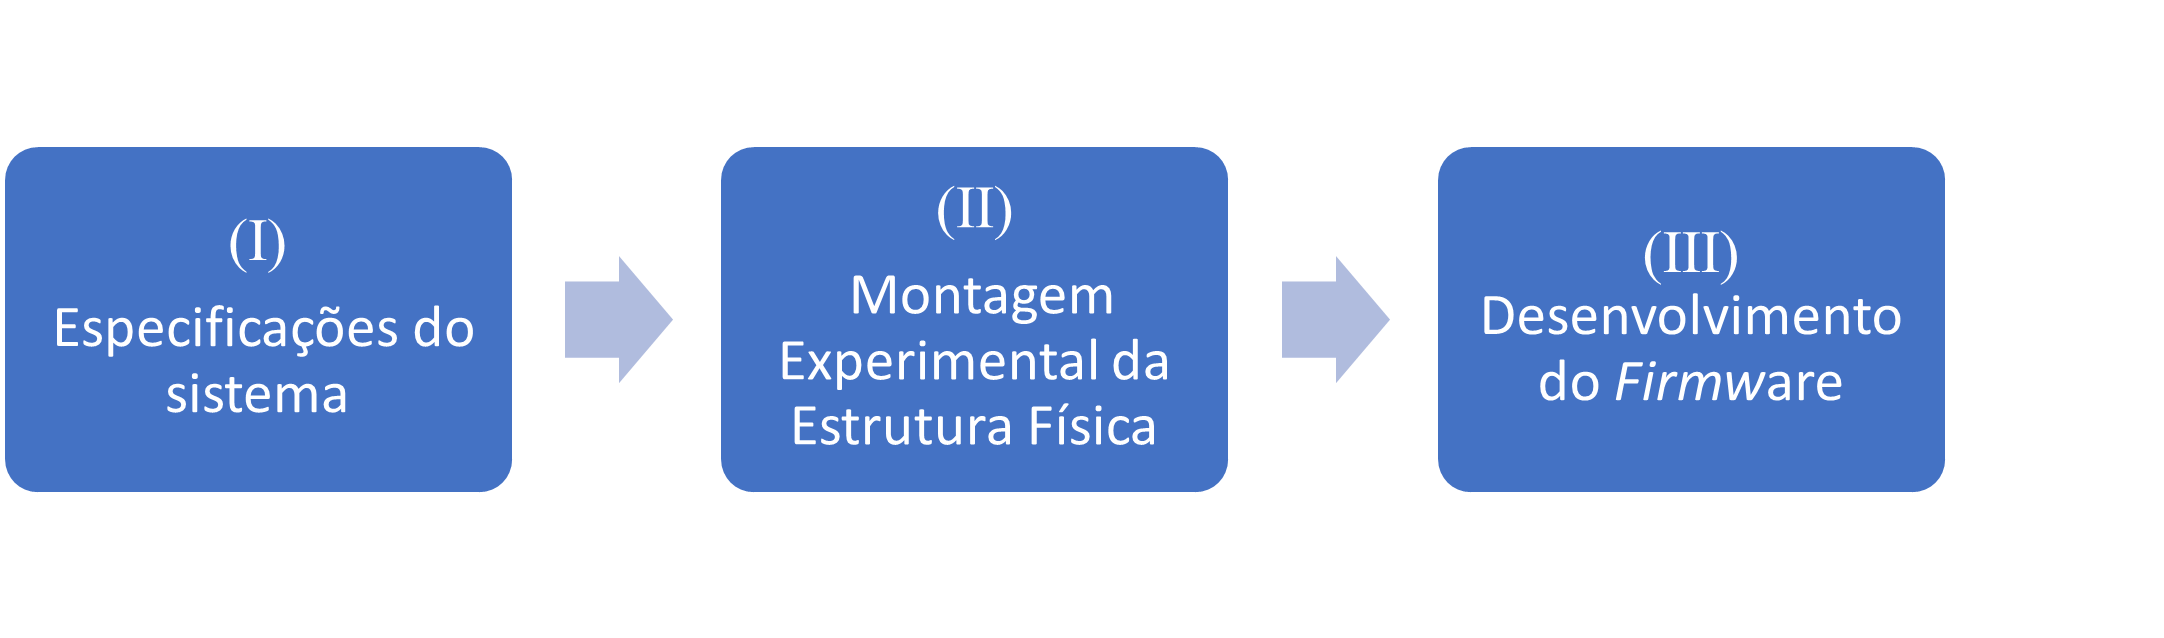
\includegraphics[width=16cm]{figuras/Metodologia.png}\\
% 	\autoria{Autoria Própria (2022)}
% 	\label{fig:Metodologia}
% \end{figure}

A metodologia adotada para o desenvolvimento do \textit{Sistema de Classificação de Doenças em Plantações de Bananeiras Utilizando Redes Neurais Convolucionais} foi estruturada em três etapas principais:

\begin{description}
    \item[(I) --] Organização e análise do conjunto de dados BananaLSD, incluindo o pré-processamento das imagens e a definição das classes de doenças a serem classificadas;
    
    \item[(II) --] Implementação da arquitetura de rede neural convolucional (\textit{ResNet-32}) e execução dos experimentos com diferentes conjuntos de dados, parâmetros e resoluções de imagem;
    
    \item[(III) --] Avaliação dos resultados obtidos por meio de métricas de desempenho como acurácia, \textit{f1-score} e área sob a curva (\textit{AUC}), complementada por análise estatística não paramétrica para validação dos resultados.
\end{description}


\section{Revisão Bibliográfica} 


Segundo \cite{RezendeArt}, as \ac{RNC} são uma das técnicas de \ac{AP} que, devido ao avanço computacional dos últimos anos, alavancaram a área de visão computacional ao possibilitar ganhos substanciais nos mais variados problemas de classificação, principalmente aqueles que envolvem imagens digitais. Nesse contexto, este trabalho propôs uma metodologia para a classificação de doenças referentes a algumas espécies de plantas, tendo como base de dados composta por imagens digitais de doenças nas plantas.

O trabalho de \cite{leite2022}, propõe que \ac{RNC} melhoram a precisão da detecção e classificação, além de permitir melhor compartilhamento de aprendizado entre diferentes conjuntos de dados. Além disso, também desenvolveu um protótipo de aplicativo para dispositivos móveis, demonstrando que o uso dessas redes pode ser empregado em pequenos dispositivos.

Para uma abordagem na aplicação de \ac{AP} na detecção da Sigatoka Amarela na produção de bananas, \cite{Deteccao_de_sigatoka_am} utilizaram \ac{RNC} profundas integradas à transferência de aprendizado. O estudo testa diferentes arquiteturas, como MobileNetV2, Inception-V3, Xception, VGG-16, ResNet50, Inception-ResNet-2 e EfficientNetB7, em um conjunto de dados composto por 6.788 imagens de folhas, sendo 941 afetadas pela doença e 981 saudáveis. 

O artigo \cite{Frutcultura} apresenta o desenvolvimento de um sistema de suporte à detecção de Sigatoka negra baseado em imagens digitais. O processo inclui a caracterização do usuário agrícola e a implementação de uma metodologia de aprendizado de máquina para classificar a doença. A validação do sistema é realizada por meio de testes laboratoriais e de campo, além de interação com o usuário agrícola.

A pesquisa de \cite{DadosArt} introduz um conjunto extenso de imagens de folhas de banana afetadas por três doenças prevalentes: Sigatoka, Cordana e Pestalotiopsis. \ac{BananaLSD} é um banco de dados que foi utilizado para desenvolver o modelo BananaSqueezeNet. O \ac{BananaLSD}  contém 937 imagens coletadas em campos de banana, que foram posteriormente aumentadas para gerar mais 1600 imagens.

Existe o trabalho de \cite{Arti3}, que implementa um sistema automatizado para monitorar o crescimento de plantas. Este trabalho combina processamento de imagem e \ac{IoT} para monitorar a planta e coletar fatores ambientais como umidade e temperatura. Junto dessa linha de pesquisa, o artigo de \cite{Art4} também utiliza a \ac{IoT} em plantas de banana com uma técnica de agrupamento K-Mean junto com sistema inteligente de chatbot. Ambos os trabalhos podem ser úteis para agricultores, botânicos, industrialistas, engenheiros de alimentos e médicos.

Para uma avaliação sobre técnicas de aprendizado de máquina aplicadas à agricultura de produção de banana, os autores \cite{Art6} fazem uma revisão sistemática da literatura. Deste modo, analisam problemas relacionados às culturas de banana, como classificação de doenças, detecção de lesões por frio, maturação, teor de umidade, entre outros. Neste estudo, os autores tentam implementar a função da arquitetura modificada do AlexNet CNN na plataforma Android para prever doenças do tomate com base na imagem da folha. Um conjunto de dados com 18.345 dados de treinamento e 4.585 dados de teste foi usado para criar o modelo preditivo.

AlexNet é uma arquitetura de rede \ac{RNC} desenvolvida por Alex Krizhevsky. Ela ganhou notoriedade por ter uma taxa de erro muito pequena. O trabalho \cite{AlexNetTomat} os autores implementará a função da arquitetura modificada do AlexNet na plataforma Android, com objetivo de prever doenças do tomate com base na imagem da folha. Um conjunto de dados com 18.345 dados de treinamento e 4.585 dados de teste foi usado para criar o modelo preditivo.

Com base nas pesquisas realizadas e na eficiência das técnicas computacionais, foram desenvolvidas várias aplicações como a área de identificação automática de doenças em plantas. Essas ferramentas são essenciais para fornecer suporte especializado, rápido e barato, contribuindo significativamente para o aumento da produção agrícola.



\section{Organização da Monografia}

Este trabalho está estruturado em seis capítulos, descritos a seguir:

\section{Organização da Monografia}

Este trabalho está dividido em seis capítulos, conforme descrito a seguir:

\begin{description}
    \item[Capítulo 1 --] Apresenta o contexto do estudo, incluindo introdução, problematica, objetivos  e trabalhos relacionados.

    \item[Capítulo \ref{cap:03} --] Aborda os fundamentos teóricos sobre aprendizado de máquina, redes neurais convolucionais e detecção de doenças em bananeiras.

    \item[Capítulo \ref{cap:04} --] Descreve a metodologia aplicada, desde a preparação dos dados até a implementação e avaliação do modelo ResNet-32.

    \item[Capítulo \ref{cap:05} --] Apresenta e discute os resultados obtidos nos experimentos realizados.

    \item[Capítulo \ref{cap:06} --] Expõe as conclusões do trabalho e sugere direções para estudos futuros.

    \item[Referências Bibliográficas --] Lista as fontes utilizadas na elaboração deste trabalho.
\end{description}


	\newpage \thispagestyle{empty}
	
	%\chapter{REVISÃO BIBLIOGRÁFICA}{}
\label{cap:02}
O Quadro \ref{tab:q1} apresenta uma descrição com os principais estudos bibliográficos utilizados como base para o presente trabalho.

\begin{quadro}
\caption{Principais referências bibliográficas utilizadas} \label{tab:q1}\\
\end{quadro}
\begin{center}
    \begin{longtable}{|p{2.5cm}|p{1.5cm}|p{4cm}|p{6cm}|}
        %\caption{Exemplo de longtable}\\
        \hline
        \centering \textbf{Autor} & \centering  \textbf{Tipo} & \centering  \textbf{Objetivo} & \centering \textbf{ Resultados} \\
        \hline
        \endfirsthead
       % \multicolumn{4}{c}%
      % {\tablename\ \thetable\ -- \textit{Continuação da tabela}} \\
       % \hline
       % \centering \textbf{Autor} & \centering  \textbf{Tipo} & \centering  \textbf{Objetivo} & \centering \textbf{ Resultados} \\
       % \hline
      %  \endhead
        \hline \multicolumn{4}{r}{\textit{Continua na próxima página}} \\
        \endfoot
        \hline \multicolumn{4}{r}{\textit{Fim do Quadro}} \\
        \endlastfoot
       \centering \citeonline{correia2016automaccao} & \centering Artigo & 
       Este trabalho apresenta uma proposta de desenvolvimento de um protótipo de baixo custo de aquisição (plataforma \textit{Arduino}\footnote{Arduino - Placa de prototipagem eletrônica de código aberto.}) para monitoramento e controle automático da irrigação, com acionamento remoto via aplicativo.

                & 
       Após testes de usabilidade com seis voluntários, 
        evidenciou-se uma boa receptividade do sistema, 
        sendo que estes não encontraram dificuldades em 
        operar o sistema.
        Houve uma redução do consumo de água 
       durante as irrigações em torno de 26,80\% no modo 
        automático do sistema.

               \\ \hline 
               \centering \citeonline{lima2019desenvolvimento} & \centering Artigo & Este artigo propõe 
            um projeto de controle automático para sistema de irrigação 
            utilizando tecnologias \ac{IoT}.
 & Com base nos testes realizados o sistema de controle é seguro. Trocando a antena do HC12 por uma antena dipolo com maior ganho foi possível alcançar a distância desejada. Dessa forma, o projeto de controle automático para sistema de irrigação desenvolvido é eficaz, eficiente e economicamente viável. \\ \hline 
               \centering \citeonline{velasco2019internet} & \centering Artigo & O principal objetivo do desenvolvimento é fornecer um protótipo de modelo com tecnologia combinada no monitoramento de uma horta para sistemas de irrigação. & Após vários testes sobre a capacidade do sistema, o aplicativo \ac{IoT} para sistemas de irrigação inteligente atendeu às necessidades dos agricultores que utilizam dispositivos \ac{IoT}. \\ \hline 
               \centering \citeonline{pisanu2020prototype} & \centering Artigo & Projetar, desenvolver e construir um protótipo de uma
plataforma eletrônica de baixo custo para monitoramento de ambiente de estufa em tempo real.
 & O protótipo da plataforma eletrônica para monitoramento do ambiente de estufa foi projetado para ser modular, tendo obtido êxito em várias combinações com \textit{firmwares}\footnote{firmware - Programa embarcado em \textit{hardware}} otimizados. \\ \hline
        \centering \citeonline{widyawati2020design} & \centering Artigo & Este artigo apresenta um sistema de monitoramento das condições ambientais em uma estufa usando a tecnologia da  \ac{IoT}. & Os resultados dos testes durante sete dias mostraram que o protótipo \ac{IoT} para sistemas de monitoramento de estufas foi capaz de funcionar bem. Isso é indicado pela porcentagem média de dados armazenados com sucesso em 99,76\% e a porcentagem média de perda ou duplicação de dados de 0,24\%.  \\ \hline 
        \centering \citeonline{friha2021internet} & \centering Artigo & Este artigo apresenta uma revisão abrangente das tecnologias emergentes para a agricultura inteligente baseada na Internet das Coisas. & Por meio de extensa pesquisa e análise conduzidas, foi possível classificar os aplicativos \ac{IoT} para agricultura inteligente em sete categorias, incluindo monitoramento inteligente, gerenciamento de água, aplicativos agroquímicos, gerenciamento de doenças, colheita inteligente, gerenciamento da cadeia de suprimentos e gerenciamento inteligente. \\ \hline 
        \centering \citeonline{marques2021plataforma} & \centering Artigo & Este artigo tem como objetivo desenvolver um sistema de coleta de 
dados, de baixo custo, para a obtenção de parâmetros relacionados à luminosidade, umidade do solo, 
umidade do ar e temperatura em ambiente agrícola.
 & A plataforma \textit{Arduino} e os sensores acessórios, mostraram-se perfeitamente aplicáveis para a aquisição e
armazenamento de dados em casas de vegetação. O protótipo de registrador de dados desenvolvido apresentou
redução de custo de 600 até 3000\% em relação aos componentes disponíveis no mercado com
funcionalidades semelhantes.
 \\ 


    \end{longtable}
\end{center}

O presente trabalho	desenvolveu um controle de irrigação no ambiente de uma estufa, semelhante ao apresentado em \citeonline{widyawati2020design}. Esta abordagem permite um maior controle das variáveis do ambiente. Em contrapartida, em \citeonline{lima2019desenvolvimento}, só é possível controlar o nível de umidade do solo, limitando as possibilidades de manipulação das condições microclimáticas, entretanto, simplificando a aplicação em campo. 

Dessa forma, o monitoramento e controle da planta foi realizado de maneira remota, por meio de \textit{software} computacional, semelhante ao apresentado em \citeonline{correia2016automaccao}, mas, o microcontrolador selecionado foi o PIC 18F4550, já que o mesmo possui capacidade de processamento adequada à aplicação.

A interface humano-máquina pode ser acessada por plataforma \textit{desktop} e por sistemas operacionais \textit{Android}\footnote{Android - Sistema operacional desenvolvido para dispositivos móveis.} ou IOS\footnote{IOS - Sistema operacional desenvolvido exclusivamente para dispositivos da \textit{Apple}}, possibilitando o monitoramento e controle do sistema de qualquer local com acesso à internet, facilitando o acompanhamento e acesso aos dados em tempo real.

	%\newpage \thispagestyle{empty}
	
	\chapter{FUNDAMENTAÇÃO TEÓRICA}{}
\label{cap:03}

A bananicultura configura-se como uma das principais atividades agrícolas do Brasil, tanto em termos econômicos quanto sociais, estando presente em todas as regiões do país e sendo praticada por produtores de diferentes escalas. Independentemente do sistema de produção adotado, a adoção de boas práticas agrícolas (BPA) e de boas práticas de fabricação (BPF) é fundamental para garantir a produção de alimentos seguros, ambientalmente responsáveis e economicamente viáveis (EMBRAPA, 2017).
Neste contexto, o presente capítulo tem como objetivo apresentar as principais doenças foliares que afetam a bananeira, detalhando suas causas, sintomas visuais e estágios de desenvolvimento. Essas informações são essenciais para compreender a base visual utilizada na classificação automática por redes neurais convolucionais.

\section{Sigatoka}

A Sigatoka, também conhecida como \textit{doença das manchas nas folhas}, é uma das principais enfermidades que acometem as plantações de bananeira, comprometendo diretamente a fotossíntese e a produtividade das plantas. Esta doença é causada por fungos do gênero \textit{Mycosphaerella}, sendo as duas espécies mais comuns a \textit{Mycosphaerella musicola}, responsável pela \textit{Sigatoka-amarela}, e a \textit{Mycosphaerella fijiensis}, causadora da \textit{Sigatoka-negra} silva2024, embrapa2017\textbf{} \cite{silva2024, embrapa2017}.

Os sintomas da Sigatoka incluem manchas amarelas nas folhas mais velhas, que gradualmente se tornam marrons e necróticas. A progressão da doença leva à morte prematura das folhas, comprometendo a fotossíntese da planta. O controle da doença envolve o uso de fungicidas, práticas culturais como a remoção de folhas infectadas e melhoria da ventilação no dossel da plantação \cite{rezende2020}. A seguir, apresentam-se as duas variantes da doença, com base nas descrições da EMBRAPA \cite{embrapa2017}.

\subsection{Sigatoka-amarela (\textit{Mycosphaerella musicola})}

\subsubsection*{Sintomas}

Os sintomas iniciais aparecem na face superior da folha, como uma leve descoloração em forma de ponto entre as nervuras secundárias da segunda à quarta folha (Figura~\ref{fig:sigatoka_amarela}A). Essas descolorações evoluem para estrias amarelas, que posteriormente tornam-se marrons. Na sequência, surgem manchas necróticas escuras, envoltas por um halo amarelo, com formato elíptico característico (Figura~\ref{fig:sigatoka_amarela}B). Na fase final, o centro da mancha torna-se deprimido, com tecido seco e coloração cinza, circundado por bordos pretos, resultando na necrose de grandes áreas foliares (Figura~\ref{fig:sigatoka_amarela}C).

\begin{figure}[h]
    \centering
    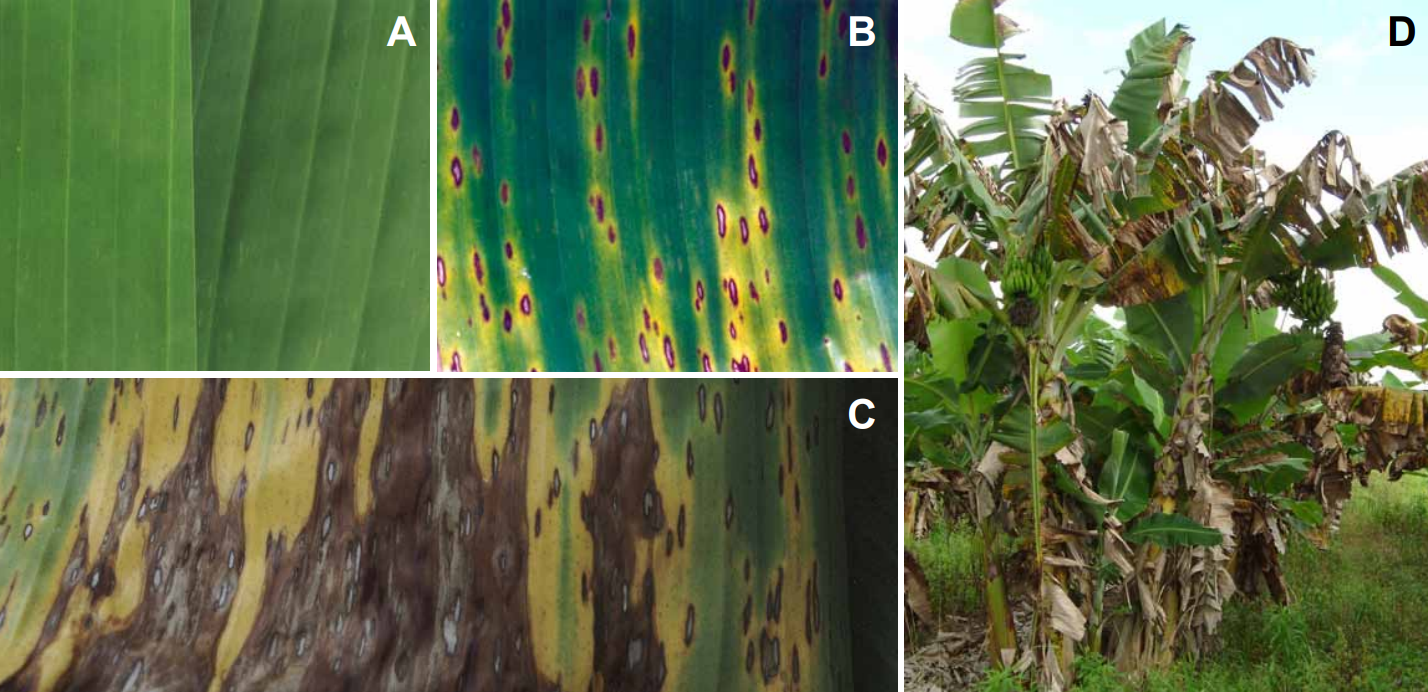
\includegraphics[width=0.9\textwidth]{figuras/capitulo 3/amarela.png}
    \caption{Sintomas da sigatokaamarela: estádios iniciais da doença
(A); manchas elípticas (B); necrose foliar (C); perdas na produção (D).
}
    \label{fig:sigatoka_amarela}
    \small{\textbf{Fonte:} EMBRAPA (2017)}
\end{figure}

\subsubsection*{Estágios de desenvolvimento}

A lesão da Sigatoka-amarela passa por seis estágios principais (Figura~\ref{fig:sigatoka_amarela_estagios}):

\begin{enumerate}
    \item \textbf{Estágio I:} ponto ou risca com até 1 mm de comprimento, com leve descoloração;
    \item \textbf{Estágio II:} estria amarelada com alguns milímetros de comprimento;
    \item \textbf{Estágio III:} estria alargada com coloração vermelho-amarronzada;
    \item \textbf{Estágio IV:} mancha oval alongada, de contornos indefinidos e coloração parda;
    \item \textbf{Estágio V:} presença de halo amarelado e início da esporulação;
    \item \textbf{Estágio VI:} mancha com centro cinza deprimido, bordos pretos e halo amarelo.
\end{enumerate}

\begin{figure}[h]
    \centering
    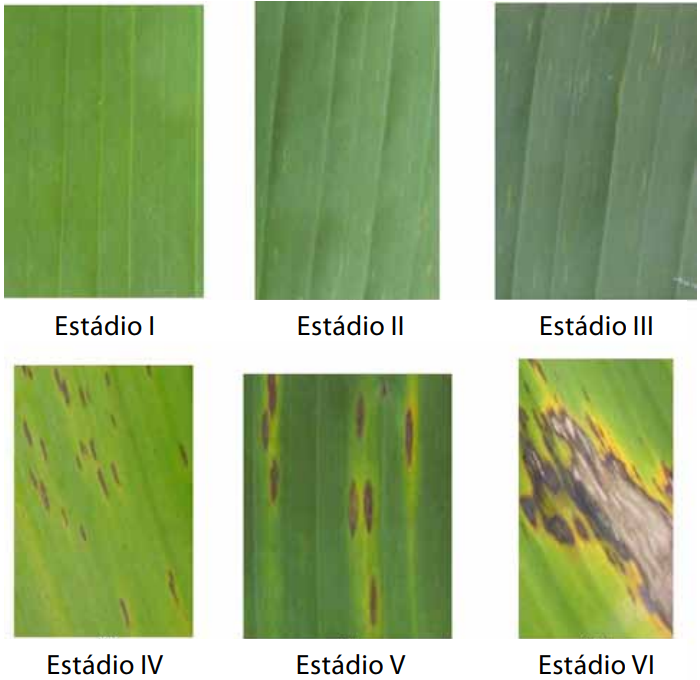
\includegraphics[width=0.7\textwidth]{figuras/capitulo 3/amarela_estagios.png}
    \caption{Estágios de desenvolvimento da lesão de Sigatoka-amarela.}
    \label{fig:sigatoka_amarela_estagios}
    \small{\textbf{Fonte:} EMBRAPA (2017)}
\end{figure}

\subsection{Sigatoka-negra (\textit{Mycosphaerella fijiensis})}

\subsubsection*{Sintomas}

A Sigatoka-negra inicia-se na \textbf{face inferior da folha}, com pontos amarelados que evoluem rapidamente para estrias marrons (Figura~\ref{fig:sigatoka_negra}A, \ref{fig:sigatoka_negra}B). Essas estrias tornam-se negras e visíveis também na face superior (Figura~\ref{fig:sigatoka_negra}C). As estrias, ao coalescerem, formam áreas extensas de necrose, e com frequência não apresentam halo amarelado. Em estágios avançados, observa-se destruição total da folha (Figura~\ref{fig:sigatoka_negra}D).

\begin{figure}[h]
    \centering
    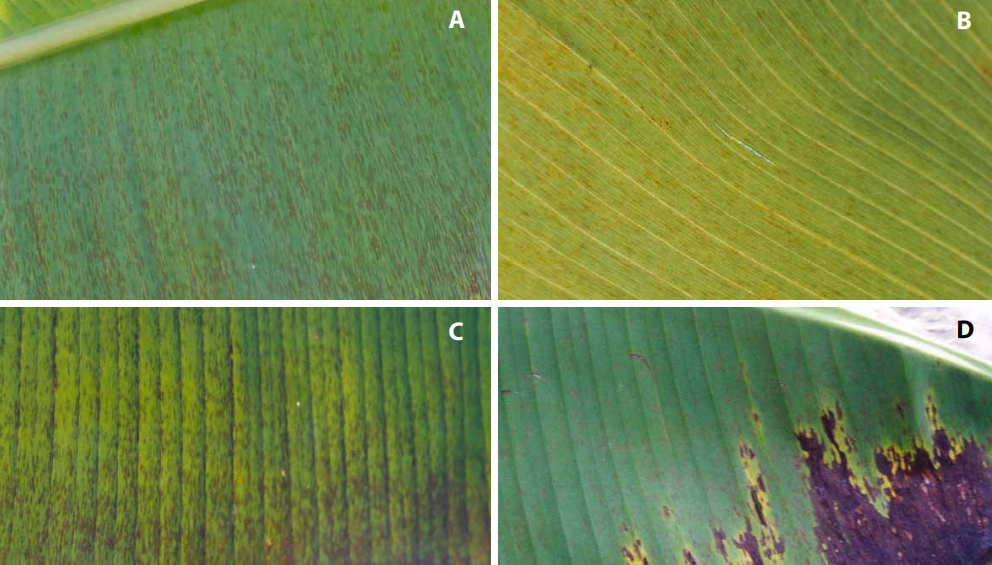
\includegraphics[width=0.7\textwidth]{figuras/capitulo 3/negra.png}
    \caption{Sintomas da Sigatoka-negra: (A, B) estrias marrons na face inferior; (C) necrose na face superior; (D) necrose total.}
    \label{fig:sigatoka_negra}
    \small{\textbf{Fonte:} EMBRAPA (2017)}
\end{figure}

\subsubsection*{Estágios de desenvolvimento}

A lesão da Sigatoka-negra também apresenta seis estágios distintos (Figura~\ref{fig:sigatoka_negra_estagios}):

\begin{enumerate}
    \item \textbf{Estágio I:} pequenos pontos amarelo-amarronzados na face inferior;
    \item \textbf{Estágio II:} estrias marrom-avermelhadas visíveis à luz;
    \item \textbf{Estágio III:} estrias de até 30 mm, quase negras, visíveis em ambas as faces;
    \item \textbf{Estágio IV:} mancha elíptica com halo aquoso marrom-claro;
    \item \textbf{Estágio V:} centro necrótico negro, levemente deprimido, com halo amarelado;
    \item \textbf{Estágio VI:} centro cinza com presença de pseudotécios (pontos negros de esporos).
\end{enumerate}

\begin{figure}[h]
    \centering
    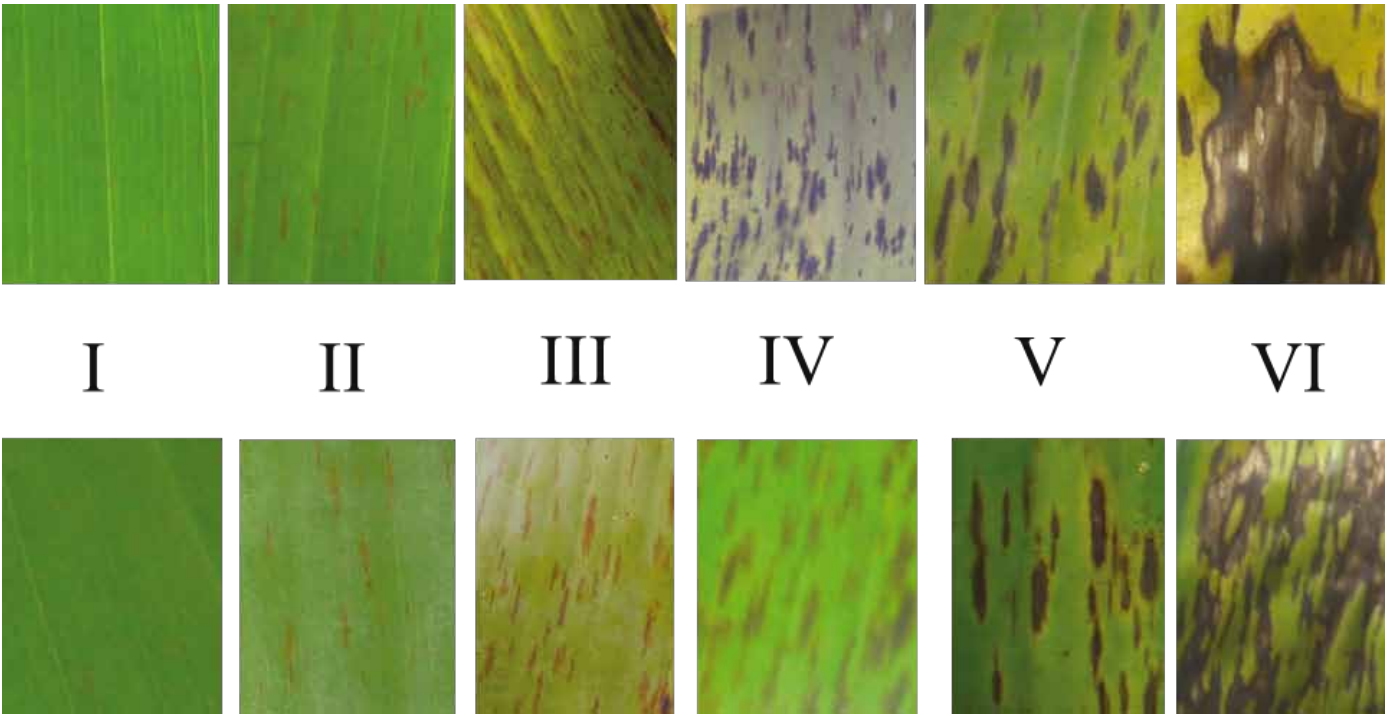
\includegraphics[width=0.8\textwidth]{figuras/capitulo 3/estagios da doenca.png}
    \caption{Estágios de desenvolvimento da lesão de Sigatoka-negra.}
    \label{fig:sigatoka_negra_estagios}
    \small{\textbf{Fonte:} EMBRAPA (2017)}
\end{figure}

\vspace{1em}
A presença de sintomas visuais progressivos e relativamente padronizados, como os apresentados pela Sigatoka-amarela e Sigatoka-negra, fundamenta a proposta de aplicação de redes neurais convolucionais (CNNs) para sua classificação automática por meio de imagens digitais.



\section{Mancha de Cordana (\textit{Neocordana musae})}

A mancha de Cordana é uma doença foliar causada pelo fungo \textit{Neocordana musae} (anteriormente conhecido como \textit{Cordana musae}), que afeta as folhas da bananeira e pode reduzir a capacidade fotossintética da planta, comprometendo a produtividade e a qualidade da produção. Embora seja considerada uma doença secundária em relação à Sigatoka, sua presença está associada ao enfraquecimento do tecido foliar e à umidade excessiva. Em muitos casos, suas lesões evoluem a partir de áreas previamente afetadas por Sigatoka, agravando o estado sanitário das folhas \cite{embrapa2017, pereira2020}.

\subsubsection*{Sintomas}

Os sintomas iniciais da mancha de Cordana podem ser confundidos com os da Sigatoka-amarela. As lesões iniciais apresentam coloração semelhante e formato elíptico, dificultando o diagnóstico visual (Figura~\ref{fig:cordana}A). À medida que evoluem, tornam-se maiores do que o habitual, embora mantenham um padrão visual similar ao das manchas de Sigatoka. Nas fases finais, as lesões atingem vários centímetros de comprimento e largura, sendo caracterizadas por \textbf{zonas concêntricas bem definidas} e circundadas por um \textbf{halo amarelo} (Figura~\ref{fig:cordana}B e \ref{fig:cordana}C).

\begin{figure}[h]
    \centering
    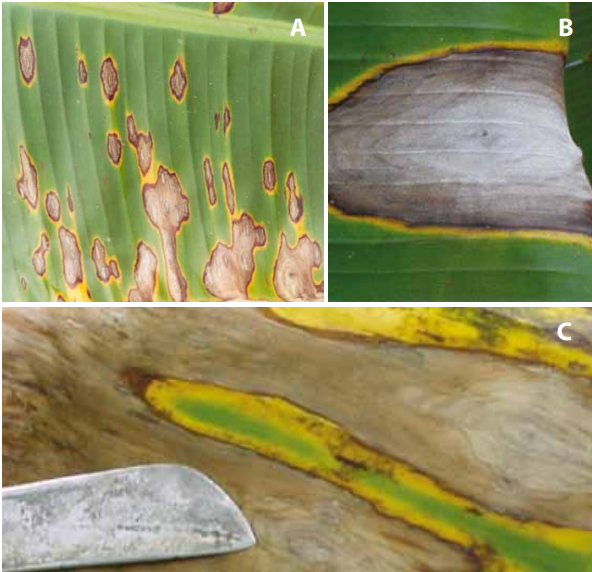
\includegraphics[width=0.5\textwidth]{figuras/capitulo 3/cardana.png}
    \caption{Mancha de Cordana: (A) lesões típicas sobre a folha; (B, C) detalhe das zonas concêntricas características.}
    \label{fig:cordana}
    \small{\textbf{Fonte:} EMBRAPA (2017)}
\end{figure}

A diferenciação entre Cordana e outras doenças foliares é um desafio importante para os produtores e especialistas. A presença de padrões visuais bem definidos, como as zonas concêntricas, contribui para a aplicabilidade de técnicas de visão computacional baseadas em aprendizado profundo, especialmente por redes neurais convolucionais.


\section{Queima foliar por \textit{Pestalotiopsis} (\textit{Pestalotiopsis palmarum})}

A queima foliar causada por \textit{Pestalotiopsis palmarum} é uma doença fúngica comum que afeta diversas espécies de plantas tropicais, incluindo a bananeira. Essa doença compromete diretamente as folhas da planta, resultando em redução da área fotossintética, prejuízo ao crescimento vegetativo e impacto negativo sobre a produção de frutos \cite{pestalotiopsis2020}.

\subsubsection*{Sintomas}

Os primeiros sintomas da infecção por \textit{Pestalotiopsis} incluem \textbf{lesões marrons encharcadas} na superfície das folhas (Figura~\ref{fig:pestalotiopsis}). Essas lesões tendem a se expandir e coalescer, formando áreas maiores de tecido necrosado. Com o avanço da doença, ocorre desfolha precoce e enfraquecimento da planta.

\begin{figure}[h]
    \centering
    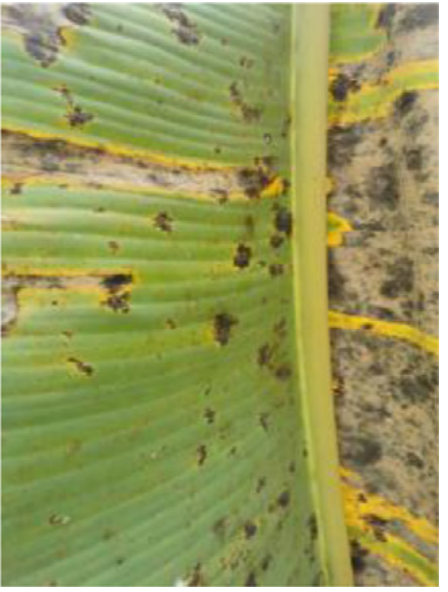
\includegraphics[width=0.5\textwidth]{figuras/capitulo 3/Pestalotiopsis.png}
    \caption{Lesões foliares causadas por \textit{Pestalotiopsis palmarum}: manchas marrons encharcadas em expansão.}
    \label{fig:pestalotiopsis}
    \small{\textbf{Fonte:} Elaborado pelo autor com base em imagens públicas de sintomas da doença.}
\end{figure}

A doença é favorecida por ambientes \textbf{quentes e úmidos}, sendo comum em regiões tropicais. Além disso, pode se espalhar pelo uso de mudas contaminadas ou material vegetativo infectado. A presença de lesões características torna viável o uso de redes neurais convolucionais na detecção automática da doença, uma vez que os padrões visuais são reconhecíveis e recorrentes em imagens foliares.



Apesar da existência de características visuais relativamente padronizadas nas folhas infectadas, a diferenciação precisa entre as doenças foliares da bananeira — como Sigatoka-amarela, Sigatoka-negra, mancha de Cordana e a queima foliar por \textit{Pestalotiopsis} — ainda representa um grande desafio. Isso se deve ao fato de que, especialmente nos estágios iniciais, os sintomas podem apresentar semelhanças visuais significativas. Dessa forma, a identificação correta muitas vezes exige o conhecimento técnico de um especialista ou a realização de exames laboratoriais específicos, o que eleva os custos e torna o processo de diagnóstico inacessível para a maioria dos pequenos e médios produtores rurais.

Cada uma dessas doenças exige estratégias de controle distintas, e um diagnóstico equivocado pode comprometer toda a lavoura, seja por atraso no manejo adequado, seja pela aplicação incorreta de defensivos. Nesse cenário, a aplicação de técnicas computacionais baseadas em aprendizado profundo, como as redes neurais convolucionais (CNNs), surge como uma alternativa promissora. Ao automatizar a classificação das doenças por meio da análise de imagens digitais, essas técnicas possibilitam diagnósticos mais rápidos, acessíveis e com maior precisão, mesmo em regiões onde o acesso a assistência técnica especializada é limitado.



\section{Banco de Dados para Detecção da Doença}


O conjunto de dados adquirido \ac{BananaLSD} possui um banco de imagens divididas em 2 categorias de folhas de bananeira: Sigatoka e saudável. As 2 classes totalizam 530 imagens. Todas as imagens foram rotuladas por um especialista em  patologia de plantas. As imagens foram todas tiradas manualmente com câmeras de smartphone em uma plantação de bananas \cite{DadosArt}. Figura \ref{fig:Fig5} representa as duas características, sendo que, a culuna amarela mostra a quantidade de imagens de sigatoka e a azul a quantidade de imagens saudáveis.  

\begin{figure}[!h]
	\centering
	\caption{Conjunto de dados adquirido \ac{BananaLSD}}
	%\vskip 5mm
	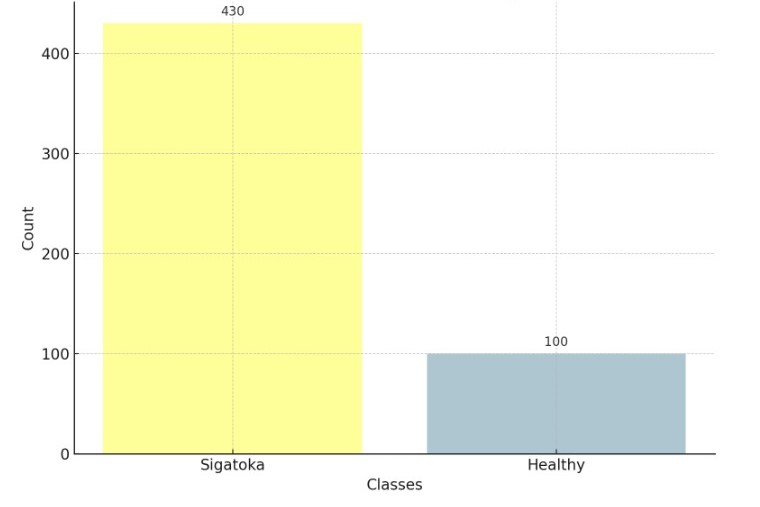
\includegraphics[width=10cm]{figuras/classes Sigatoka e Healthy.jpg}\\
	\autoria{Autoria Própria (2024).}
	\label{fig:Fig5}
\end{figure}

A pasta do conjunto de dados contém duas pastas, uma para o conjunto original e outra para o conjunto aumentado. Ambas essas pastas contêm duas subpastas - sigatoka e saudável - uma para cada uma das classes.


% COMECA AQUI --------------------------------------------------------
\section{Aprendizagem de Máquina e Redes Neurais Artificiais}
\label{sec:aprendizagem-maquina}

% Definindo o ambiente para aprendizagem de máquina
A aprendizagem de máquina é um campo da inteligência artificial que desenvolve algoritmos capazes de aprender padrões a partir de dados, permitindo previsões ou classificações sem programação explícita \cite{mitchell1997machine}. No contexto da bananicultura, a aprendizagem de máquina é aplicada para identificar doenças foliares, como Sigatoka, mancha de Cordana e Pestalotiopsis, a partir de imagens digitais, otimizando o diagnóstico e reduzindo perdas agrícolas \cite{RezendeTese}, \cite{DadosArt}.

O aprendizado supervisionado, foco deste trabalho, utiliza dados rotulados (ex.: imagens de folhas associadas a classes de doenças) para treinar modelos que mapeiam entradas (pixels) para saídas (rótulos). O treinamento minimiza uma função de custo por meio de algoritmos como \textit{gradient descent} e \textit{backpropagation} \cite{Rumelhart1986}. A avaliação do desempenho, descrita na Seção \textcolor{red}{\ref{sec:metodologia}}, utiliza métricas como acurácia (\(Ac\)) e matriz de confusão, definidas pelas Equações \ref{eq:acuracia} e \ref{eq:erro}:

\begin{equation}
Ac = \frac{\sum_{i=1}^m n_{i,i}}{\sum_{i=1}^m \sum_{j=1}^m n_{i,j}}
\label{eq:acuracia}
\end{equation}

\begin{equation}
Cf = 1 - Ac
\label{eq:erro}
\end{equation}

\subsection{Redes Neurais Artificiais}
\label{subsec:rna}

% Definindo o ambiente para RNAs
As redes neurais artificiais (RNAs) são modelos computacionais inspirados no cérebro humano, compostos por neurônios artificiais interconectados que processam informações para realizar tarefas como classificação \cite{Haykin2001}. Uma RNA é formada por camadas de entrada, ocultas e saída, com conexões ponderadas por pesos ajustados durante o treinamento \cite{RezendeTese}.

A Figura \ref{fig:neuron} ilustra um neurônio artificial, que combina entradas \(x_i\) com pesos \(w_i\), adiciona um \textit{bias} \(b\), e aplica uma função de ativação \(f\) (ex.: ReLU) para gerar a saída \(y\):

\begin{equation}
y = f\left(\sum_{i=1}^n w_i x_i + b\right)
\label{eq:neuron}
\end{equation}

\begin{figure}[h]
    \centering
    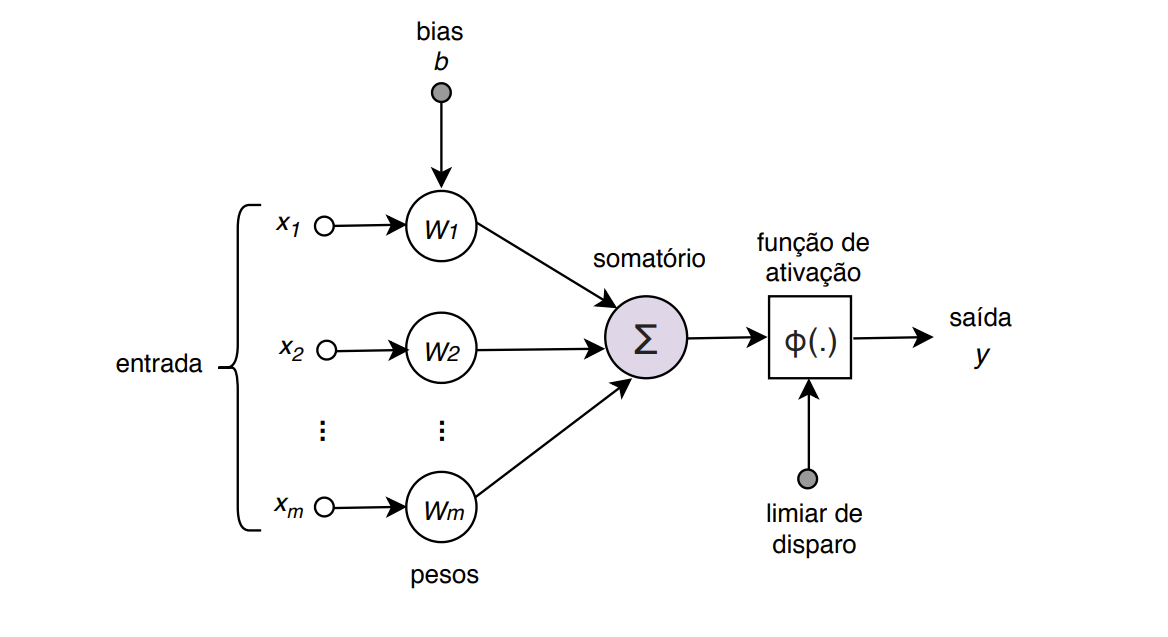
\includegraphics[width=0.8\textwidth]{figuras/NeuronioArtificial.png}
    \caption{Estrutura de um neurônio artificial, com entradas \(x_i\), pesos \(w_i\), \textit{bias} \(b\), e função de ativação \(f\) gerando a saída \(y\).} 
    Adaptado de \cite{RezendeTese}.
    \label{fig:neuron}
\end{figure}








RNAs são eficazes para modelar relações não lineares, sendo amplamente utilizadas em tarefas de reconhecimento de padrões, como a identificação de doenças em plantas \cite{Goodfellow2016}. No entanto, para imagens, as RNAs tradicionais são limitadas, exigindo arquiteturas especializadas como as redes neurais convolucionais (CNNs) \cite{leite2022}.

\section{Redes Neurais Convolucionais}
\label{sec:cnns}

% Definindo o ambiente para CNNs
As redes neurais convolucionais (CNNs) são projetadas para processar dados estruturados, como imagens, utilizando operações de \textit{convolução} para extrair características locais (ex.: bordas, texturas) \cite{LeCun1998}. No contexto deste trabalho, as CNNs são aplicadas para classificar imagens do conjunto BananaLSD, identificando padrões visuais de doenças como Sigatoka, Cordana e Pestalotiopsis \cite{DadosArt}.

\subsection{Estrutura de uma CNN}
\label{subsec:estrutura-cnn}

% Definindo a estrutura geral de uma CNN
Uma CNN é composta por:

\begin{itemize}
    \item \textbf{Camadas de Convolução}: Aplicam filtros (\textit{kernels}) para gerar mapas de características, destacando padrões como manchas ou estrias em folhas. A Figura \ref{fig:convolution} ilustra a operação de convolução.
    \item \textbf{Camadas de \textit{Pooling}}: Reduzem a dimensionalidade espacial (ex.: \textit{max pooling}), aumentando a invariância a transformações \cite{Goodfellow2016}.
    \item \textbf{Camadas Totalmente Conectadas}: Combinam características para a classificação final (ex.: saudável ou doente) \cite{RezendeTese}.
    \item \textbf{Funções de Ativação}: Introduzem não linearidades (ex.: ReLU) para modelar relações complexas \cite{Krizhevsky2012}.
\end{itemize}



A Figura \ref{fig:cnn} apresenta a arquitetura geral de uma CNN, com camadas de convolução, \textit{pooling} e totalmente conectadas, utilizada para classificar doenças em bananeiras.

\begin{figure}[h]
    \centering
    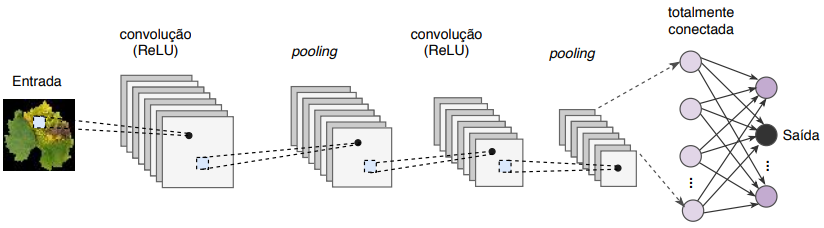
\includegraphics[width=0.9\textwidth]{figuras/capitulo 3/cnn.png}
    \caption{Arquitetura de uma CNN, processando imagens de folhas para classificar doenças. Adaptado de \cite{RezendeTese}.}
    \label{fig:cnn}
\end{figure}



\begin{figure}[h]
    \centering
    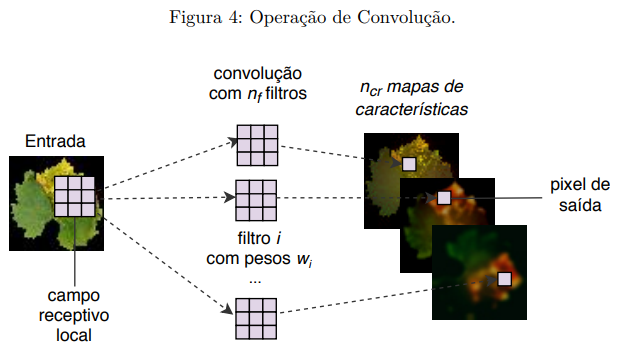
\includegraphics[width=0.8\textwidth]{figuras/capitulo 3/convolution_process.png}
    \caption{Operação de convolução, onde um filtro é aplicado a uma imagem para gerar um mapa de características. Adaptado de \cite{RezendeTese}.}
    \label{fig:convolution}
\end{figure}








%INICIO--------------------------------------------------------------------------------------------------------------------



\subsection{Arquitetura AlexNet}
\label{subsec:alexnet}

A AlexNet, proposta por \cite{Krizhevsky2012}, representou um marco no aprendizado profundo ao vencer o desafio ImageNet Large Scale Visual Recognition Challenge (ILSVRC) de 2012, destacando-se pela eficácia das redes neurais convolucionais (CNNs) em tarefas de classificação de imagens. Com aproximadamente 61 milhões de parâmetros, a AlexNet estabeleceu um novo padrão para arquiteturas de visão computacional \cite{Krizhevsky2012}.

A arquitetura da AlexNet é composta por oito camadas principais: cinco camadas convolucionais seguidas por três camadas totalmente conectadas, conforme ilustrado na Figura \ref{fig:alexnet}. As camadas convolucionais 1, 2 e 5 são seguidas por operações de \textit{max pooling}, que reduzem a dimensionalidade espacial e aumentam a invariância a transformações locais \cite{Goodfellow2016}. As camadas convolucionais 3 e 4 são diretamente conectadas, sem operações intermediárias. A camada final utiliza a função de ativação \texttt{softmax} com 1000 unidades, correspondendo às classes do desafio ImageNet \cite{Krizhevsky2012}.

A função de ativação ReLU (\(f(x) = \max(0, x)\)) é aplicada nas primeiras sete camadas, acelerando o treinamento ao introduzir não linearidades e mitigando o problema do desaparecimento do gradiente em comparação com funções como \textit{sigmoid} \cite{Braga2024}. Para reduzir o \textit{overfitting}, a AlexNet emprega \textit{dropout} com probabilidade de 50\% nas duas primeiras camadas totalmente conectadas, desativando neurônios aleatoriamente durante o treinamento para melhorar a generalização \cite{Hinton2012}. Além disso, utiliza \textit{overlapping pooling} com janelas de 3x3 e \textit{stride} de 2, permitindo maior captura de características espaciais em comparação com \textit{pooling} tradicional \cite{Krizhevsky2012}.

\begin{figure}
    \centering
    \includegraphics[width=0.9\textwidth]{images/alexnet_architecture.png}
    \caption{Arquitetura simplificada da AlexNet, com cinco camadas convolucionais, \textit{max pooling} e três camadas totalmente conectadas. Fonte: autoria própria (2024).}
    \label{fig:alexnet}
\end{figure}

A AlexNet também implementa aumento de dados (\textit{data augmentation}), como translações e espelhamentos horizontais, para enriquecer o conjunto de treinamento. Uma inovação significativa foi o uso de duas GPUs em paralelo, dividindo as camadas convolucionais em dois caminhos para acelerar o treinamento \cite{Krizhevsky2012}. Essas características, combinadas com sua profundidade, tornaram a AlexNet uma referência em arquiteturas de CNNs.


%fim alex nbet--------------------------------------------------------------------------------------------------------------------


























\subsection{Vantagens das CNNs na Bananicultura}
\label{subsec:vantagens-cnns}

% Definindo as vantagens das CNNs
As CNNs oferecem benefícios para a classificação de doenças foliares \cite{LeCun2015}:

- **Extração Automática de Características**: Aprendem padrões diretamente dos pixels, eliminando a necessidade de \textit{feature engineering} manual \cite{RezendeTese}.
- **Invariância Espacial**: Operações de \textit{pooling} permitem reconhecer sintomas independentemente de sua posição na imagem \cite{Goodfellow2016}.
- **Robustez**: Técnicas como ampliação de dados (ex.: rotação, ajuste de brilho) aumentam a generalização, como descrito na Seção \ref{sec:metodologia} \cite{Leite2022}.

No presente trabalho, as CNNs (ex.: AlexNet, ResNet-32) classificam imagens do BananaLSD, apoiando o diagnóstico precoce em regiões como Bom Jesus da Lapa \cite{Silva2024}.



	\newpage \thispagestyle{empty}
	
	

\chapter{METODOLOGIA}{}
\label{cap:04}

Neste capítulo, é descrito a metodologia que foi adotada no desenvolvimento do trabalho. O processo de treinamento do modelo de classificação de imagens, a descrição do banco de dados utilizado, a arquitetura e o funcionamento detalhado do modelo. Além disso, as ferramentas computacionais de \textit{software} e \textit{hardware} e, por fim, apresenta-se a metodologia escolhida para avaliar os resultados obtidos.

\section{Banco de dados}

O banco de dados foi extraído do artigo BananaLSD: \textit{A banana leaf images dataset for classification of banana leaf diseases using machine learning}~\cite{DadosArt}. Este conjunto de dados contém 937 imagens originais de folhas de bananeiras, divididas em quatro classes: Pestalotiopsis, Sigatoka, Cordana e folhas saudáveis. As imagens foram capturadas em condições naturais, utilizando três câmeras de smartphones, para que houvesse a maior diversidade possível no dataset em termos de iluminação e ângulos das fotos~\cite{DadosArt}.

Para o treinamento do modelo neste trabalho, são utilizadas apenas as classes Sigatoka e folhas saudáveis. A seleção dessas classes se deu para focar no desenvolvimento de um modelo que possa diferenciar entre folhas infectadas por Sigatoka e folhas saudáveis, já que a Sigatoka é considerada uma das doenças que causam mais prejuízos nas plantações de banana. A classe Sigatoka, no dataset original, contém 473 imagens, enquanto a classe de folhas saudáveis possui 129 imagens. 

\subsection{Processamento dos dados}
As imagens são de alta qualidade, portanto, foi necessário reduzi-las para um tamanho de 224x224 pixels, uma resolução mais apropriada para a construção do modelo. Em seguida, foi realizada a ampliação do conjunto das imagens redimensionadas. Modelos de aprendizado profundo tendem a ser mais eficientes quando as classes contêm mais amostras~\cite{DadosArt}. Um modelo treinado com imagens capturadas de apenas uma perspectiva tende a ser tendencioso. A ampliação garante diversidade no conjunto de dados e corrige o desbalanceamento de dados presente. As seguintes técnicas de ampliação foram aplicadas para aumentar o conjunto de dados bruto.

\begin{enumerate}
    \item Cortes: As imagens são cortadas em várias outras, reduzindo o tamanho e expandindo o conjunto de dados obtido. 
    \item Rotação horizontal: Normalmente rotacionar não é tão natural para RNC, mas para o caso em especifico não altera o aprendizado. A implementação desse aumento de dados é direta, simples de implementar e demonstrou sua eficácia na utilização deste trabalho~\cite{DadosArt}.
    \item Ajuste de contraste: Para as imagens muito claras ou muito escuras, este ajuste é necessário para corrigir vieses de iluminação.  
\end{enumerate} 

Utilizando essa metodologia foi possível um incremento de 400 imagens. Como demonstrado na Figura \ref{fig:Pastas}, as imagens foram alocadas em duas pastas: uma pasta com o conjunto aumentado e outra com o conjunto original. A pasta com o conjunto aumentado será utilizada para o treinamento do modelo, enquanto a outra pasta será usada para validação.

\begin{figure}[!h]
	\centering
	\caption{Organização das Pastas}
	%\vskip 5mm
	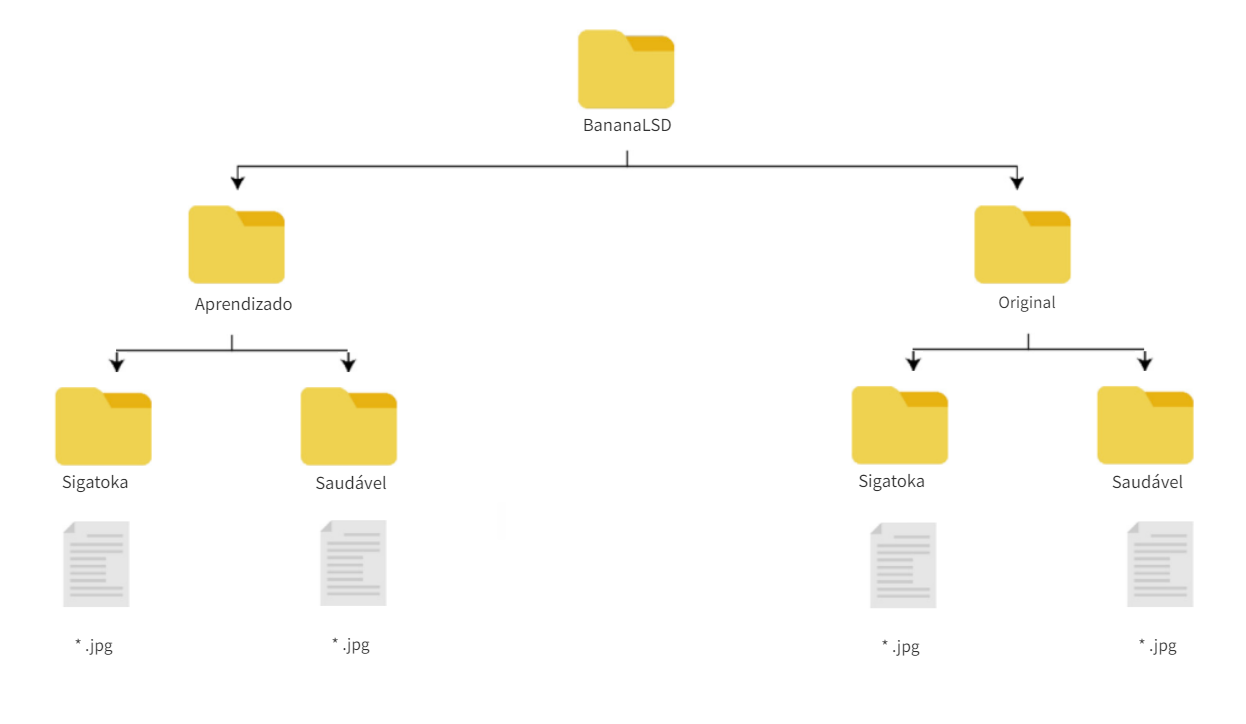
\includegraphics[width=11cm]{figuras/Pastas.png}\\
	\autoria{Autoria Própria (2024)}
	\label{fig:Pastas}
\end{figure}

\section{Implementação do Aprendizado de Máquina}
Para a tarefa de classificar imagens de folhas de bananeira, foi escolhido utilizar \ac{RNC}, já que são especialmente eficazes para reconhecimento de padrões em imagens. Isso acontece porque as \ac{RNC}s conseguem capturar características espaciais e hierárquicas da estrutura geral das imagens.

A decisão de usar \ac{RNC}s também se justifica pelos resultados positivos que elas já demonstraram em estudos anteriores sobre a detecção de doenças em plantas. Além disso, elas são capazes de lidar bem com grandes volumes de dados e com a complexidade das imagens, o que é exatamente necessário para o projeto.

Na Figura \ref{Fig:RezendeMet}, apresenta-se um diagrama detalhado que ilustra cada etapa do processo metodológico. Esse diagrama ajuda a entender a estrutura e organização do trabalho, de modo a facilitar a apresentação do objetivo de desenvolver uma classificação eficaz.

\begin{figure}[!h]
	\centering
	\caption{Metodologia para a classificação de imagens de doenças em plantas.}
	%\vskip 5mm
	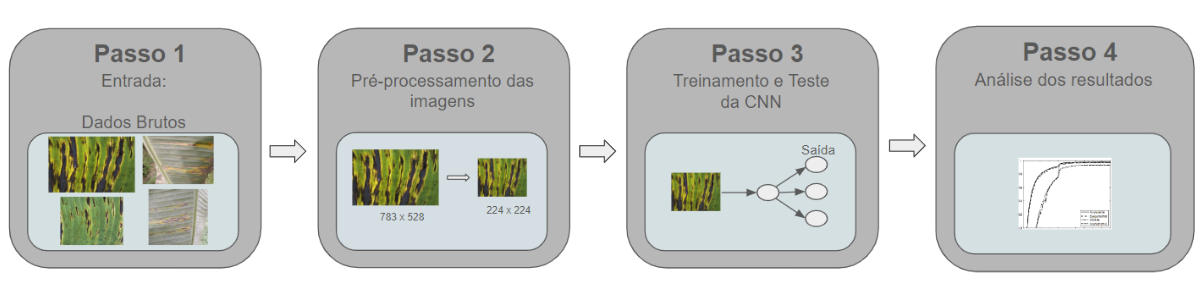
\includegraphics[width=15cm]{figuras/RezendeMetodos.png}\\
	\autoria{Autoria Própria (2024)}
	\label{Fig:RezendeMet}
\end{figure}

Primeiro, começamos selecionando a base de dados que será usado como entrada para o algoritmo. Em seguida, passamos para o pré-processamento das imagens, uma etapa importante em que ajustamos todas as imagens com as técnicas apresentadas, adaptamos todas para terem o mesmo tamanho e também removemos aquelas que poderiam atrapalhar a análise.

Com todos os dados padronizados, inicia-se a fase de treinamento e teste das RNCs, momento em que as redes começam a extrair as características mais relevantes das imagens. Por fim, realiza-se a análise de desempenho dos resultados, avaliando-se o comportamento das RNCs. Caso alguma anomalia seja detectada, ajustam-se os parâmetros necessários e reinicia-se o treinamento da rede.

\subsection{Escolha do Modelo de \ac{RNC}}
No início, apesar de as Redes Neurais Convolucionais serem amplamente conhecidas nas comunidades de visão computacional e aprendizado de máquina, elas não se tornaram imediatamente predominantes na área. Esse cenário mudou radicalmente em 2012, quando a AlexNet, uma \ac{RNC} com 8 camadas, conquistou o Desafio de Reconhecimento Visual em Grande Escala ImageNet com uma ampla vantagem~\cite{Art4}. Desde então, essa rede demonstrou pela primeira vez que o aprendizado profundo poderia superar os métodos projetados manualmente.

Conforme ilustrado na Figura~\ref{Fig:ArquitAlexnet}, a arquitetura da AlexNet é composta por cinco camadas convolucionais, seguidas por três camadas totalmente conectadas. Nas duas primeiras camadas e na quinta, cada uma é acompanhada por uma camada de max-pooling. Já a terceira e a quarta camadas são conectadas diretamente, sem nenhuma outra estrutura intermediária. A última camada da rede é utilizado a função de ativação softmax com 1000 unidades, correspondendo a cada rótulo possível.

\begin{figure}[!h]
	\centering
	\caption{Arquitetura Simplificada da Alexnet.}
	%\vskip 5mm
	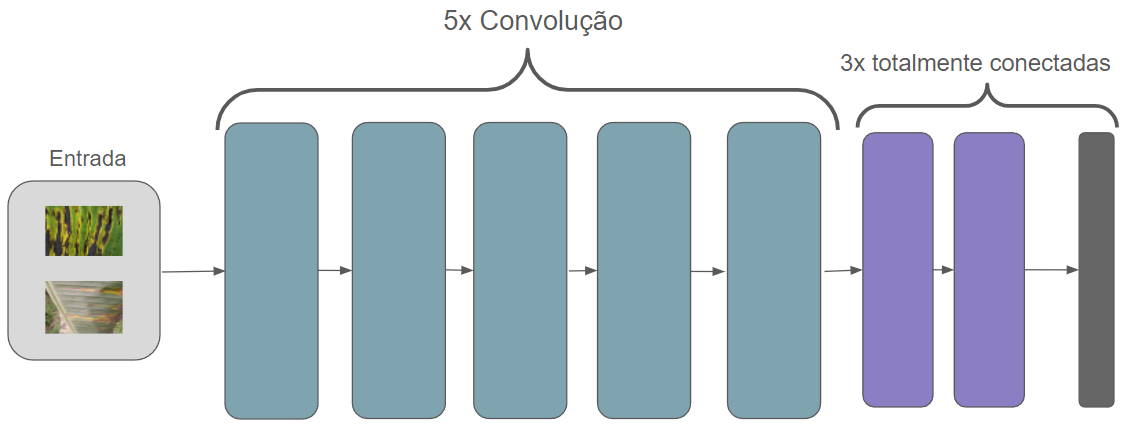
\includegraphics[width=15cm]{figuras/ArquitAlexnet.png}\\
	\autoria{Autoria Própria (2024)}
	\label{Fig:ArquitAlexnet}
\end{figure}

A arquitetura AlexNet utiliza funções de ativação \ac{ReLU} nas primeiras sete camadas da rede neural. Essas funções de ativação são conhecidas por acelerar o processo de treinamento ao introduzir não-linearidades, permitindo que a rede aprenda a representar funções complexas de forma mais eficiente.

O \textit{overfitting} ocorre quando a rede aprende a memorizar padrões específicos dos dados de treino, apresentando bom desempenho apenas nesses casos específicos, mas falhando ao generalizar para novos dados. Uma das principais estratégias utilizadas na AlexNet para combater o \textit{overfitting} é o \textit{dropout}. Essa técnica funciona ao desligar aleatoriamente neurônios durante o treinamento, com uma probabilidade de 50\% \cite{braga2021avaliacao}. Esse desligamento aleatório dos neurônios altera efetivamente a arquitetura da rede para cada entrada, ajudando a evitar que a rede se torne excessivamente dependente de qualquer neurônio ou conjunto de neurônios específicos.

\section{Metodologia de Avaliação dos Resultados}
A avaliação do desempenho de uma rede neural artificial projetada é uma etapa crucial para assegurar a qualidade dos sistemas de classificação. Existem diversas abordagens para verificar a eficácia do classificador desenvolvido.

As principais métricas aplicadas na análise de desempenho do sistema projetado foram a \ac{MC} e a  \ac{Ac}. A Figura~\ref{FIG:matriz} ilustra um exemplo de \ac{MC}, onde as classificações corretas aparecem na diagonal principal, enquanto as outras posições da matriz indicam erros de classificação. Somando-se os valores de cada linha $i$ que não estão na diagonal principal, obtêm-se os \ac{FP} da classe $i$, que representam as vezes em que o modelo previu incorretamente a classe $i$. Por outro lado, ao somar os elementos de cada coluna $j$, excluindo-se as células da diagonal principal, obtêm-se os \ac{FN} da classe $j$, que indicam objetos pertencentes à classe $i$ classificados erroneamente como de outras classes. Os \ac{TN} são determinados somando os elementos restantes, após a exclusão da linha e coluna correspondentes à classe $i$ \cite{silva2022sistema}.

\begin{figure}[!h]
	\centering
	\caption{Matriz de confusão.}
	%\vskip 5mm
	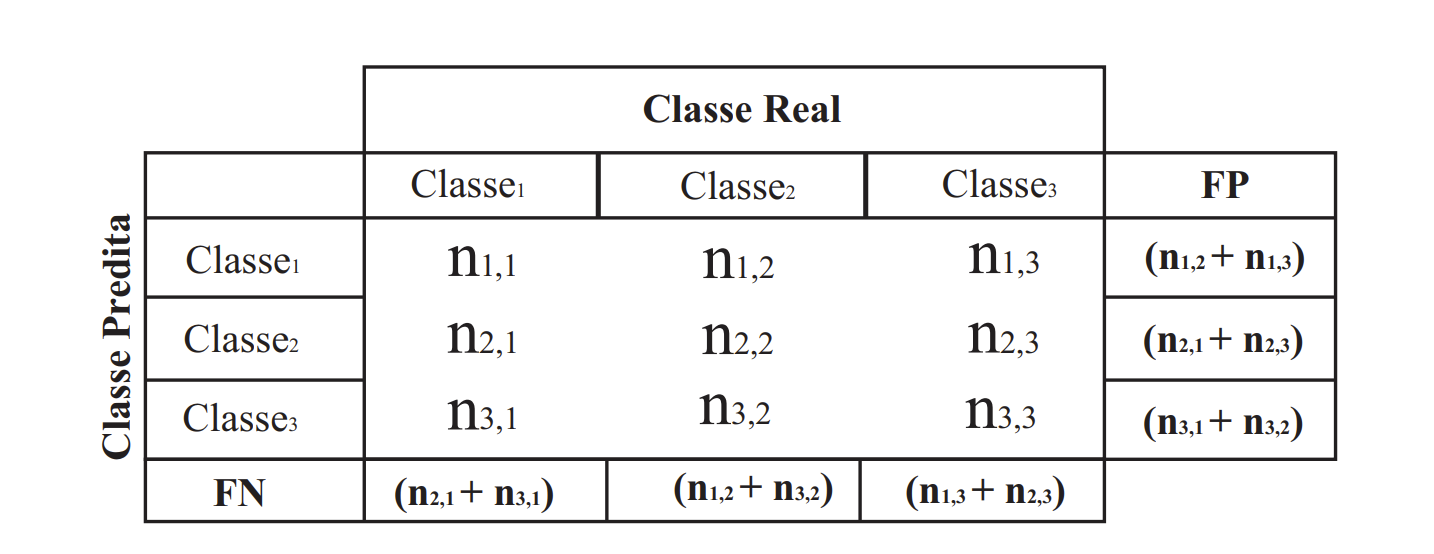
\includegraphics[width=13cm]{figuras/confusion1.png}\\
	\autoria{\cite{silva2022sistema}}
	\label{FIG:matriz}
\end{figure}

Diversas métricas de desempenho podem ser derivadas da matriz de confusão para avaliar o classificador desenvolvido. A \ac{Ac} é uma dessas métricas e representa a performance geral do modelo, indicando a proporção de acertos em relação ao número total de classificações realizadas (Equação~\ref{eq:1}). Já o erro de classificação ($Cf$) pode ser calculada pela Equação~\ref{eq:2}, expressando a relação entre as classificações incorretas e o total de classificações \cite{silva2022sistema}.   

\begin{equation}
\label{eq:1}
Ac = \frac{\sum_{i=1}^{m} n_{i,j}}{\sum_{i=1}^{m}\sum_{j=1}^{m}n_{i,j}}
\end{equation}

\begin{equation}
\label{eq:2}
Cf = 1 - Ac
\end{equation}


\section{Especificação de Máquina e Software}
As especificações da máquina utilizada incluem uma CPU Ryzen 7 5700X de 8 núcleos e 16 threads, com frequência de 3.2 GHz, e uma memória RAM de 16 GB. Para o treinamento, foi utilizada uma GPU AMD Radeon RX 580 com interface de memória de 8 GB GDDR5 de 256 bits.

O ambiente de desenvolvimento utilizado neste trabalho incluiu o Anaconda, que facilitou a gestão de pacotes e ambientes, o Jupyter Notebook para o desenvolvimento e execução interativos dos códigos, e a biblioteca PyTorch, configurada com suporte a GPUs para acelerar o treinamento de modelos.

% \begin{equation}
% Ac = \frac{\sum_{i=1}^{m} n_{i,j}}{\sum_{i=1}^{m} \sum_{j=1}^{m} n_{i,j}}
% \end{equation}


% O modelo AlexNet foi treinado ao longo de 100 épocas, com um batch size de 120 e utilizando a função de perda cross entropy. O uso do otimizador Adam com uma taxa de aprendizado inicial de 0.0001, ao invés do SGD proposto no artigo original, foi crucial para garantir a convergência do treinamento. Observou-se que o uso do SGD, conforme os parâmetros originais, não produziu resultados satisfatórios, indicando que os hiperparâmetros requerem ajustes específicos para diferentes datasets e contextos.

% Durante o treinamento, a acurácia foi monitorada em intervalos regulares. A implementação logou os valores de perda e acurácia no TensorBoard, permitindo uma análise visual da performance do modelo. A acurácia apresentou melhorias consistentes ao longo das épocas, confirmando a capacidade da AlexNet de aprender as características das imagens e diferenciá-las entre as duas classes. No entanto, a precisão exata do modelo ao final das 100 épocas não foi explicitada no código, mas pode ser inferida a partir dos logs gerados.

% Uma característica importante desta implementação foi a análise dos gradientes e dos parâmetros do modelo em pontos regulares durante o treinamento. Isso permitiu a identificação de possíveis problemas, como gradientes desvanecendo ou explodindo, e ajudou a assegurar que o treinamento estava progredindo corretamente. A análise das distribuições de gradientes e pesos no TensorBoard contribuiu para uma melhor compreensão do comportamento do modelo durante o treinamento.

% O uso de um agendador de taxa de aprendizado (StepLR) que reduziu a taxa de aprendizado em um fator de 10 a cada 30 épocas foi eficaz em refinar o treinamento do modelo. Este método ajudou a evitar que o modelo ficasse preso em mínimos locais e melhorou a capacidade do AlexNet de generalizar, ao permitir ajustes mais finos na fase final do treinamento.


% A função de visualização de algumas imagens do conjunto de dados permitiu verificar a correta aplicação das transformações e a adequação das imagens para o treinamento. Esse passo é importante para garantir que o pipeline de dados está funcionando corretamente e que as imagens estão sendo processadas conforme esperado.

% O salvamento regular de checkpoints ao final de cada época permitiu preservar o estado do modelo, possibilitando retomar o treinamento de um ponto intermediário, se necessário. Isso é essencial em treinamentos longos para mitigar a perda de progresso devido a falhas ou interrupções inesperadas.

% Em resumo, a implementação do AlexNet e os resultados obtidos demonstram a eficácia da rede para tarefas de classificação de imagens, mesmo em datasets menores e com menos classes, como o utilizado neste experimento. O uso de ferramentas como o TensorBoard para monitoramento contínuo e ajustes no treinamento se mostrou vital para alcançar uma boa performance. Contudo, é importante destacar que o ajuste fino dos hiperparâmetros, como a escolha do otimizador, desempenha um papel crucial para a adaptação do modelo a diferentes contextos e datasets.

% A exploração futura pode incluir testes com diferentes taxas de aprendizado, otimizadores, e o uso de técnicas de regularização mais avançadas para melhorar ainda mais a generalização do modelo.

% \newpage



% \subsection{Módulo sensor}

% Para a aquisição de dados do ambiente foram utilizados sensores de temperatura, umidade do solo e umidade relativa do ar. Como mencionado no capítulo anterior, o sensor de temperatura escolhido para o projeto foi o DHT-22, que possui características descritas na Tabela \ref{tab:my-table4}, pois suas especificações de precisão, estabilidade, durabilidade e condições operacionais se encaixam nos requisitos do projeto. O seu protocolo de 1- Barramento permite a conexão de múltiplos sensores em uma única entrada do microcontrolador, isso permite com que sejam utilizados vários sensores em pontos distintos da estufa, obtendo valor mais abrangente da temperatura ambiente sem a necessidade de ocupar mais portas lógicas do microcontrolador.


% \begin{table}[!h]
% \centering
% \caption{Características de temperatura do sensor DHT-22.
% }
% \label{tab:my-table4}
% \begin{tabular}{c|c}
% \hline
% \textbf{Características}    & \textbf{Valor}                                                                                                               \\ \hline
% Alimentação                 & 3,0V a 6,0V                                                                                                                  \\ \hline
% Temperatura de operação     & -55°C a 125°C                                                                                                                \\ \hline
% Precisão entre -10°C a 85°C & 0,5°C                                                                                                                        \\ \hline
% Pinagem                     & \begin{tabular}[c]{@{}c@{}}Vermelho: Tensão de corrente contínua (VCC)\\ Amarelo: Dados\\ Preto: Referência/GND\end{tabular} \\ \hline
% Comprimento do cabo         & 1 m                                                                                                                          \\ \hline
% Protocolo                   & 1- Barramento                                                                                                                \\ \hline
% \end{tabular}
% \\
% \autoria{\cite{gomes2017calibraccao}}
% \end{table}

% Para mensurar a umidade relativa do ar foi utilizado o sensor DHT-22, suas características de funcionamento são expostas na Tabela \ref{tab:my-table5}, esse sensor possui a capacidade de medir tanto a umidade relativa do ar, quanto a temperatura ambiente, tem como vantagem o baixo custo e a grande quantidade de trabalhos desenvolvidos com ele na literatura.

% \begin{table}[!h]
% \centering
% \caption{Características de umidade do ar do sensor DHT-22.
% }
% \label{tab:my-table5}
% \begin{tabular}{c|c}
% \hline
% \textbf{Características} & \textbf{Valor}                                                                                              \\ \hline
% Alimentação              & 3,0V a 6,0V                                                                                                   \\ \hline
% Umidade de operação      & 0 a 100\%                                                                                                   \\ \hline
% Precisão                 & 2\%                                                                                                         \\ \hline
% Pinagem                  & \begin{tabular}[c]{@{}c@{}}Pino 1: Tensão de corrente contínua (VCC)\\ Pino 2: Dados\\ Pino 3: Referência/GND\end{tabular} \\ \hline
% Sinal de saída           & Sinal digital via barramento único                                                                          \\ \hline
% \end{tabular}
% \\
% \autoria{\cite{gomes2017calibraccao}}
% \end{table}

% Foi desenvolvido um módulo sensor contendo os componentes necessários para o funcionamento do DHT-22, Sendo composto por um resistor de 4,7K que foi ligado entre o pino de alimentação positiva e o pino de dados, sendo utilizado para garantir que o sinal ficará em um nível lógico conhecido quando o pino não estiver enviando sinal, também foi utilizado um capacitor de 100nF entre os pinos de alimentação positiva e negativa, para filtrar ruídos de alta frequência que podem distorcer o sinal de dados, as ligações foram realizadas de acordo com a Figura \ref{fig:LDHT22}. 

% \begin{figure}[!h]
% 	\centering
% 	\caption{Esquema de ligação do módulo DHT22}
% 	%\vskip 5mm
% 	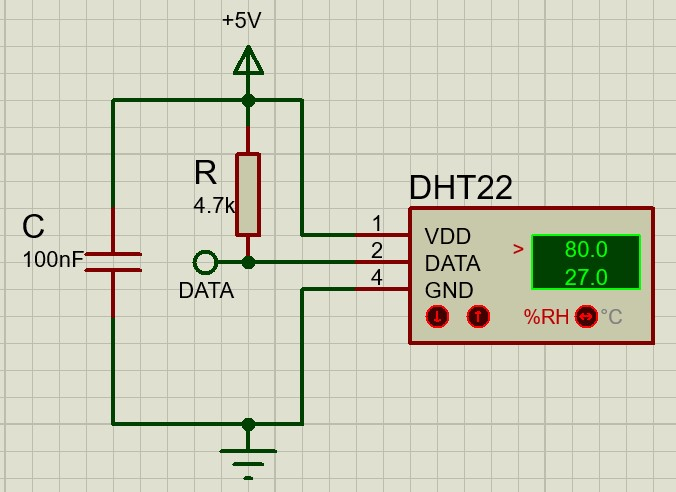
\includegraphics[width=7cm]{figuras/image.png}\\
% 	\autoria{Autoria própria}
% 	\label{fig:LDHT22}
% \end{figure}

% Para garantir uma boa conexão entre os componentes, o módulo foi desenvolvido em uma placa de circuito impresso e seus componentes foram isolados com o uso de um tubo termo retrátil, foram utilizados fios de alumínio cobreado para prolongar os pinos do módulo e aumentar a distancia em que ele pode ficar do módulo de condicionamento de sinais, o protótipo é apresentado na Figura \ref{fig:MDHT22}.


% \begin{figure}[!h]
% 	\centering
% 	\caption{Módulo DHT22}
% 	%\vskip 5mm
% 	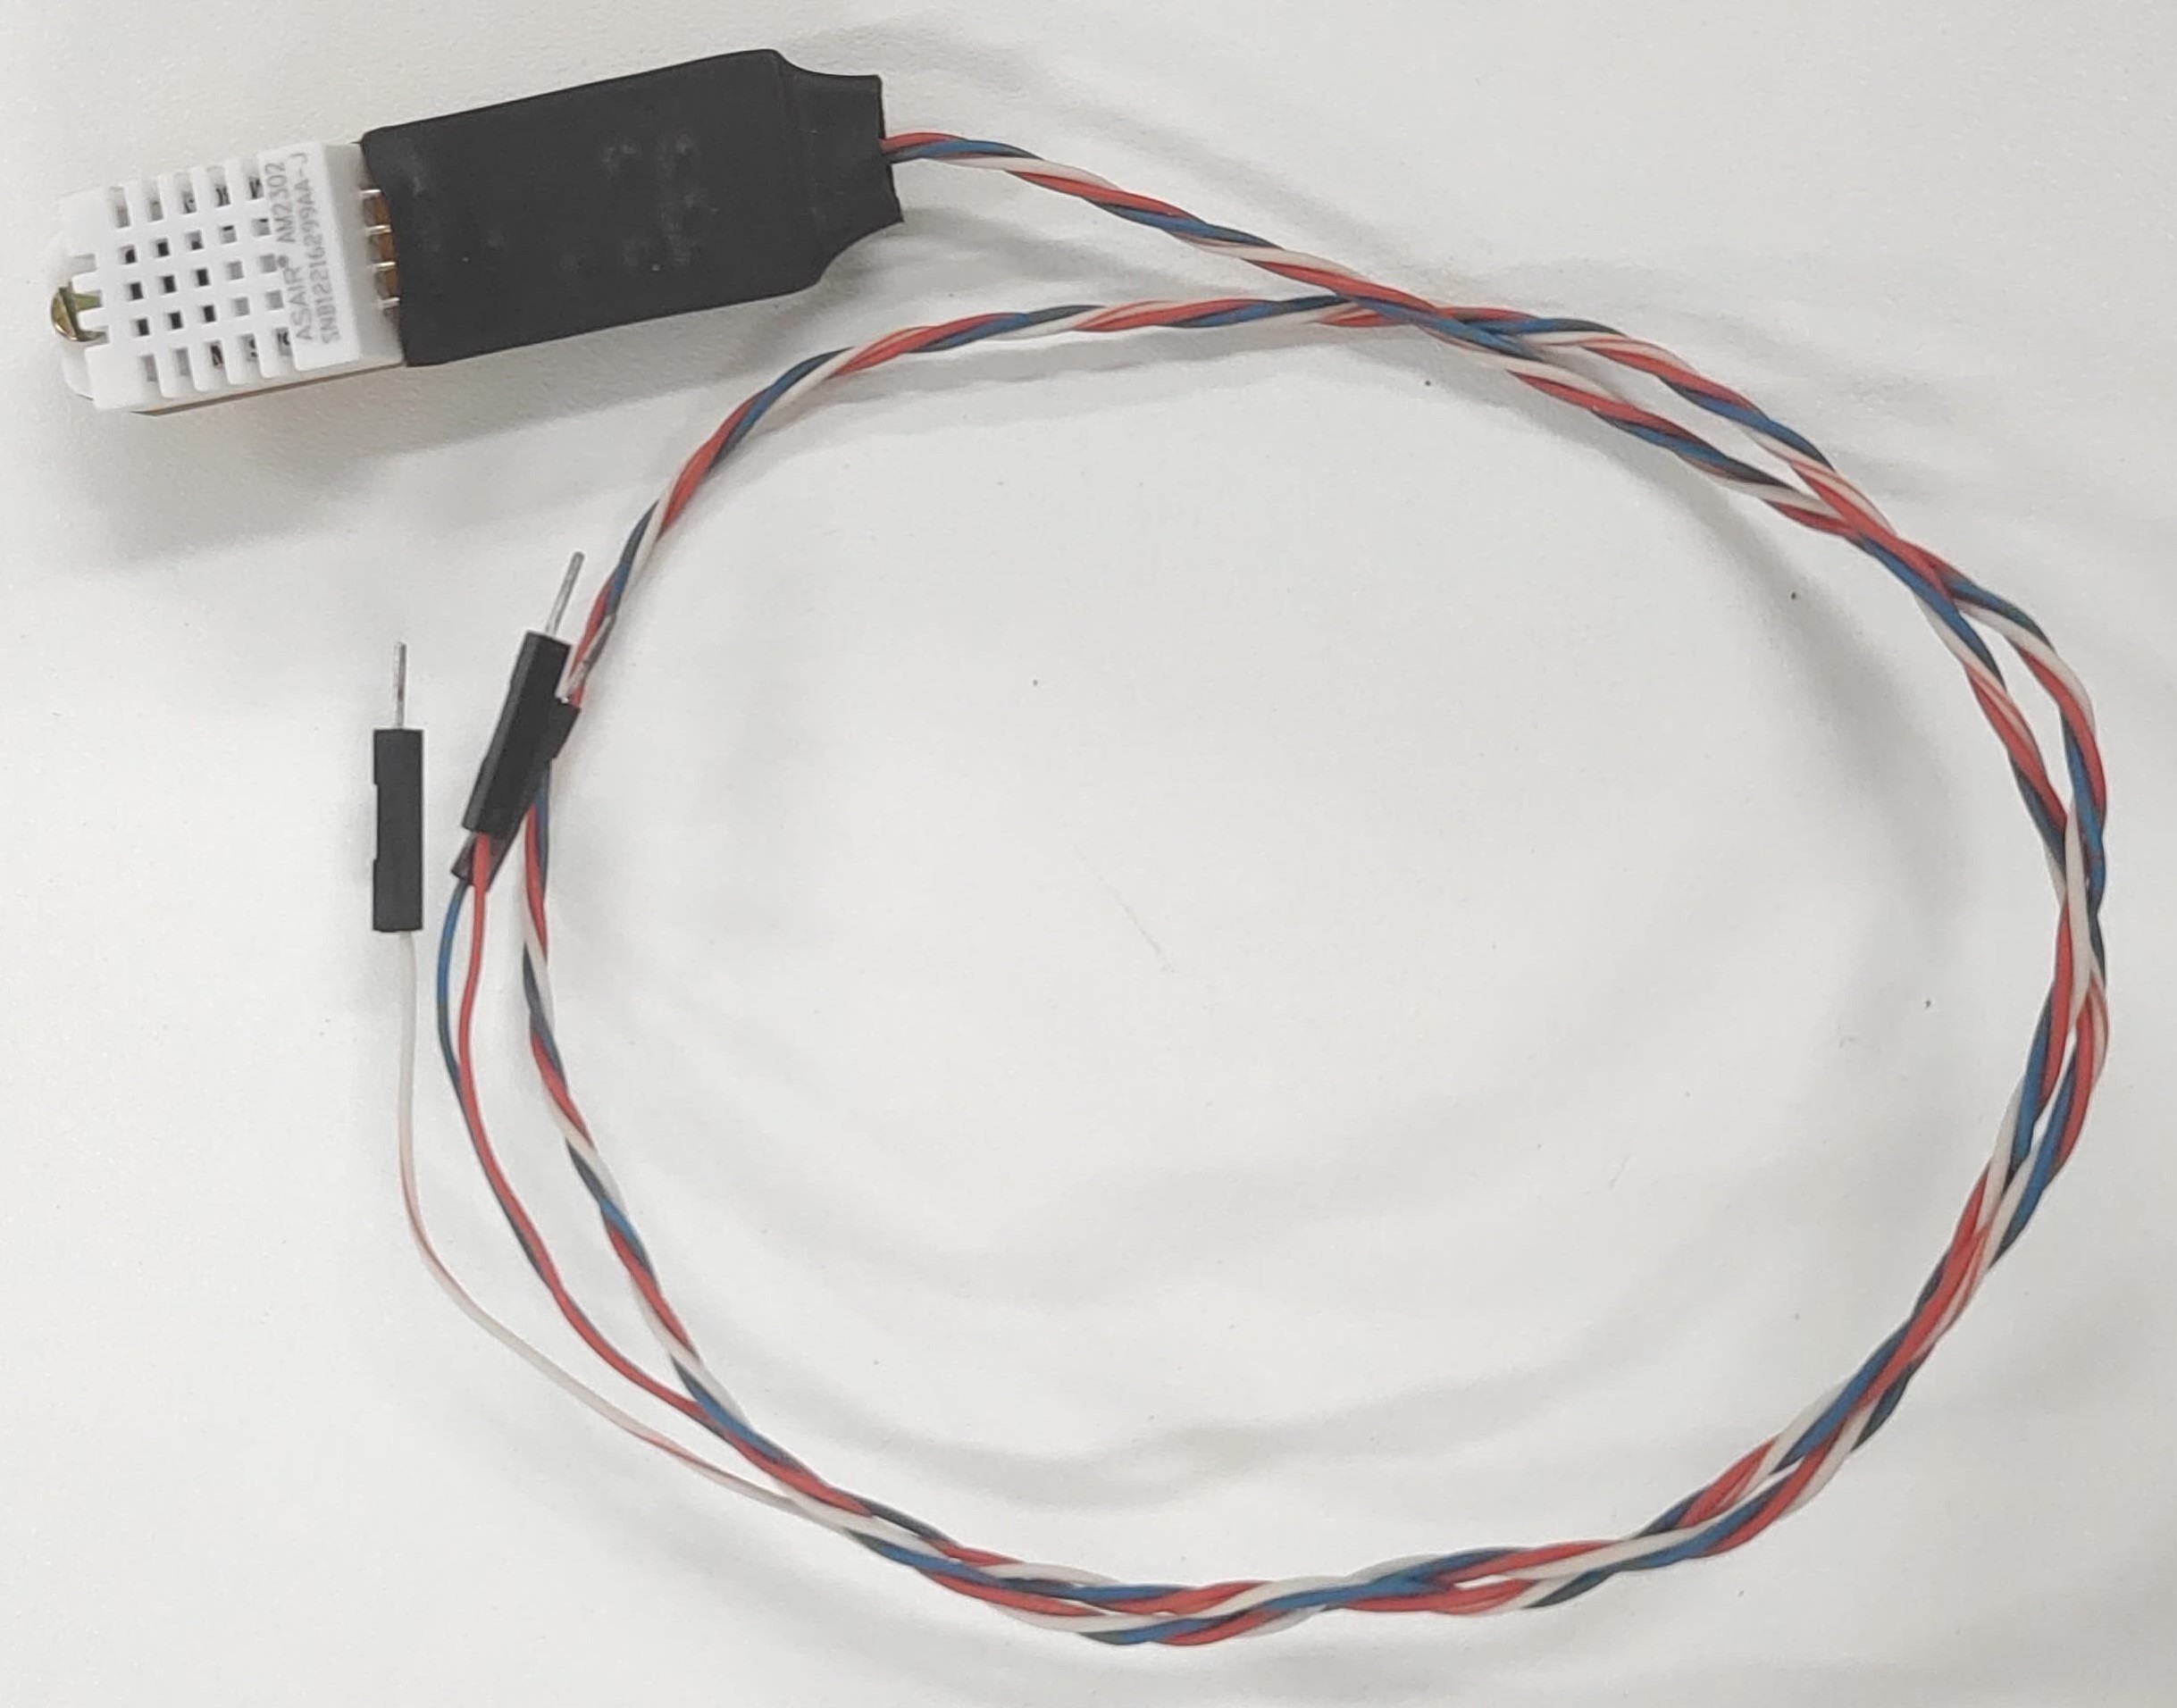
\includegraphics[width=6cm]{figuras/MEUDHT22.jpeg}\\
% 	\autoria{Autoria própria}
% 	\label{fig:MDHT22}
% \end{figure}

% O sensor de umidade do solo HD-38 possui encapsulamento de metal, tornando resistente a corrosões causadas pelo contato contínuo com o solo, como apresentado na Tabela \ref{tab:my-table6}, suas características o tornam ideal para o projeto.


% \begin{table}[!h]
% \centering
% \caption{Características do sensor HD-38.
% }
% \label{tab:my-table6}
% \begin{tabular}{c|c}
% \hline
% \textbf{Características} & \textbf{Valor}                                                                                              \\ \hline
% Alimentação              & 3,3V a 12,0V                                                                                                \\ \hline
% Umidade de operação      & 0 a 100\%                                                                                                   \\ \hline
% Precisão                 & 1\%                                                                                                         \\ \hline
% Pinagem                  & \begin{tabular}[c]{@{}c@{}}Pino 1: Tensão de corrente contínua (VCC)\\Pino 2: Dados\\Pino 3: Referência/GND\end{tabular} \\ \hline
% Comprimento do cabo      & 1 m                                                                                                         \\ \hline
% \end{tabular}
% \\
% \autoria{\cite{gomes2017calibraccao}}
% \end{table}

% Os sensores foram posicionados em pontos estratégicos na estufa, visando a captura de dados de maneira homogênea. Cada módulo de sensores é composto por um sensor DHT-22 e um HD-38. O módulo foi conectado fisicamente ao circuito de condicionamento de sinais, que fornece a alimentação dos sensores.  

% \subsection{Módulo atuador}

% O módulo de atuadores é conectado fisicamente ao circuito de condicionamento de sinais, que é responsável por transmitir os comandos a serem executados pelos atuadores, além de captar o estado atual de cada atuador. A composição do módulo depende das características do local onde é aplicado, podendo conter relés para acionamento de cargas como motores, ventiladores e bombas, além de válvulas solenoides para controlar o fluxo de água. Para os testes realizados, foi utilizado um módulo relé de quatro canais, como visto na Figura \ref{fig:RELE}.

% \begin{figure}[!h]
% 	\centering
% 	\caption{Módulo relé}
% 	%\vskip 5mm
% 	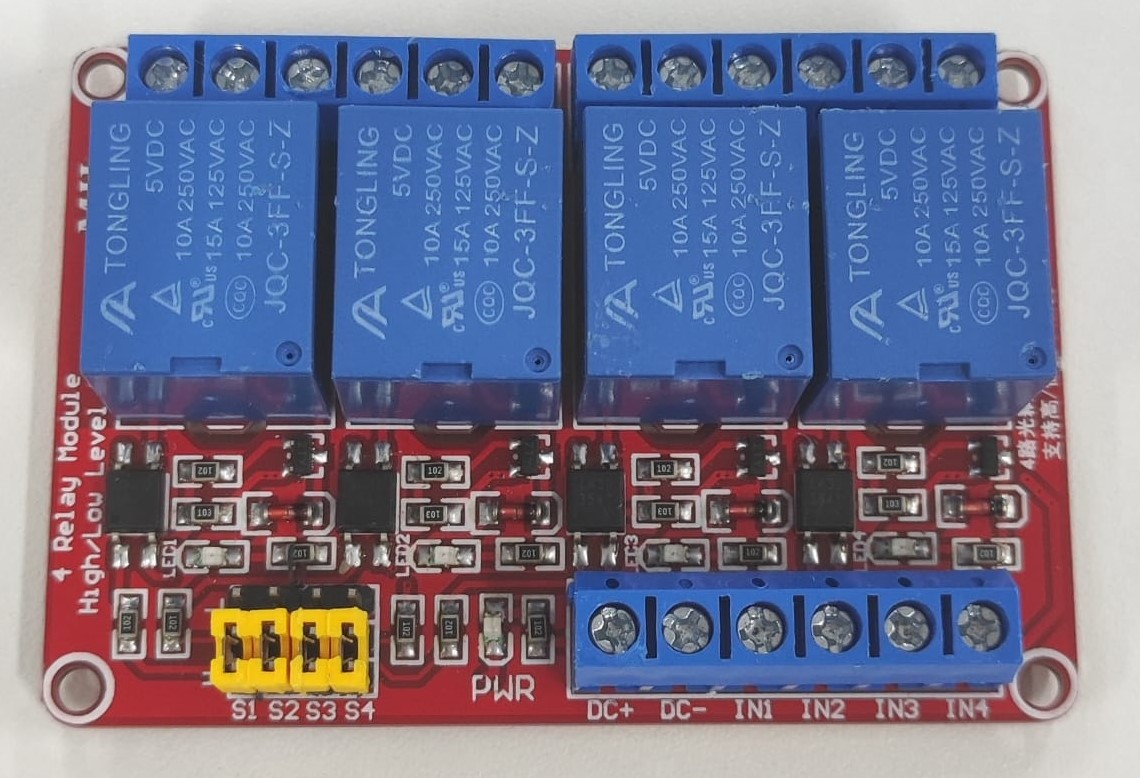
\includegraphics[width=8cm]{figuras/RELE.jpeg}\\
% 	\autoria{Autoria própria}
% 	\label{fig:RELE}
% \end{figure}

% \subsection{Circuito de condicionamento de sinais}

% O circuito de condicionamento de sinais tem função muito importante no projeto, ele é responsável por captar os dados dos sensores, condiciona-los e processa-los. Esta etapa realiza o controle dos atuadores, de maneira independente do módulo central, esse controle ocorre independente de conexão com internet ou \ac{Wi-Fi}, implicando maior confiabilidade ao sistema, pois perdas de conexão não afetam as funções de aquisição de dados dos sensores e controle dos atuadores.

% Este circuito é composto por microcontrolador PIC18F4550 e circuito eletrônico necessário para o seu funcionamento, que é fornecido pela placa \textit{microStart}, que conta com oscilador externo de 20 MHz, entrada USB tipo B e conector P4 para alimentação de 6V a 15V contínuos, a placa utilizada é vista na Figura \ref{fig:PICP}. 

% \begin{figure}[!h]
% 	\centering
% 	\caption{Placa PIC}
% 	%\vskip 5mm
% 	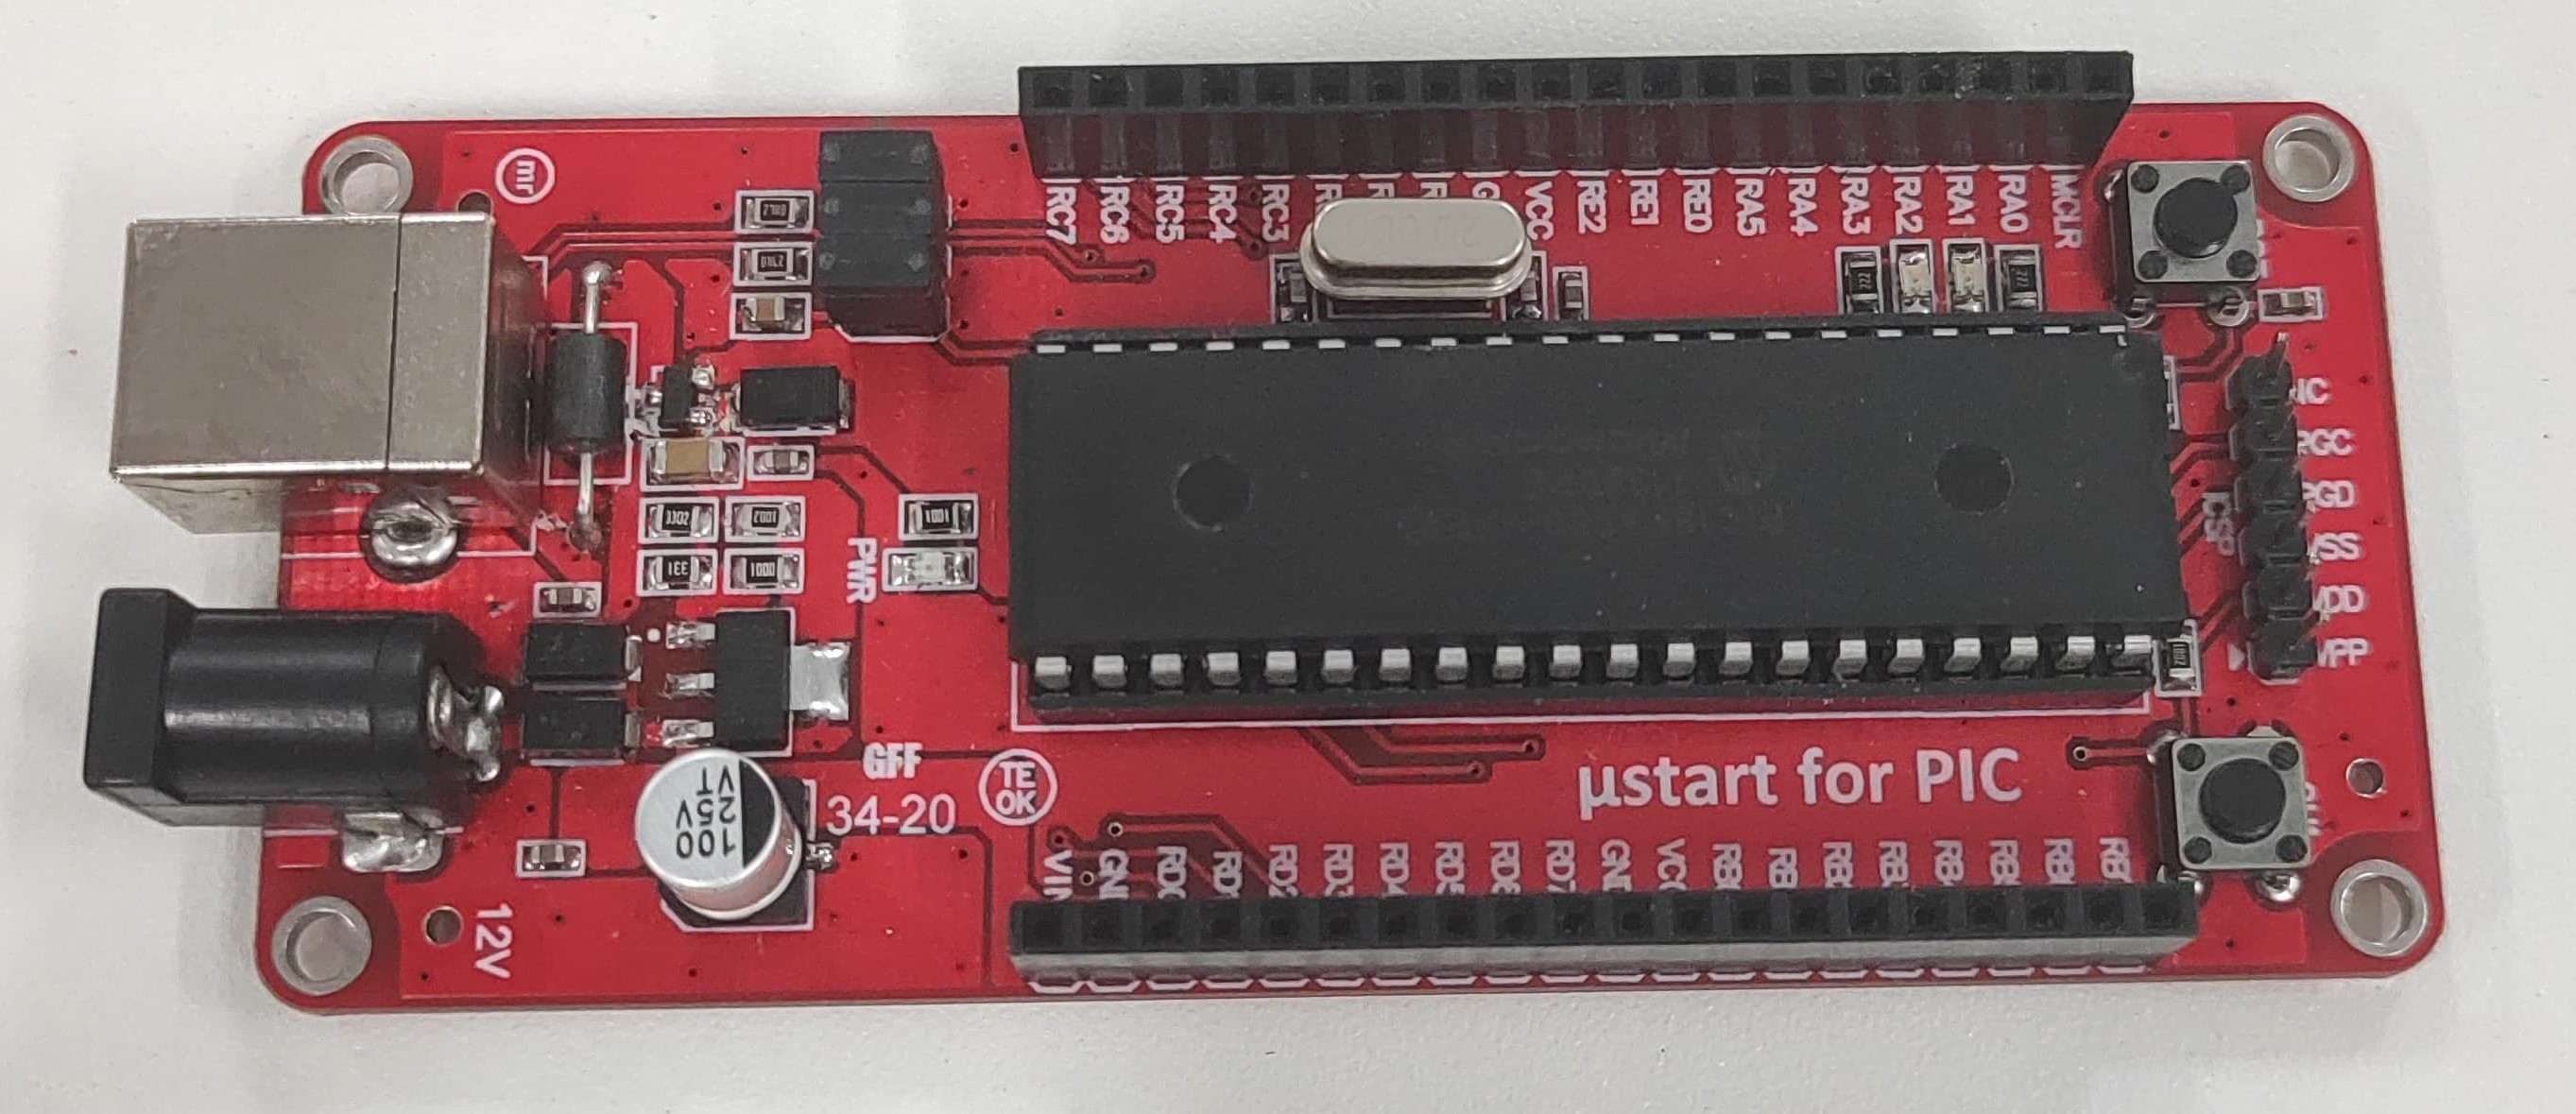
\includegraphics[width=10cm]{figuras/PLACAPIC.jpeg}\\
% 	\autoria{Autoria própria}
% 	\label{fig:PICP}
% \end{figure}

% Conta também com circuito de comunicação via radiofrequência para se conectar com o módulo central, além de fonte de alimentação composta por módulos fotovoltaicos e baterias, caso a estufa esteja em uma localidade que não tenha disponibilidade de energia elétrica, na Figura \ref{fig:ligac} é apresentado o esquema de ligação entre os componentes do circuito.

% \begin{figure}[!h]
% 	\centering
% 	\caption{Esquema de ligação do módulo de condicionamento de sinais}
% 	%\vskip 5mm
% 	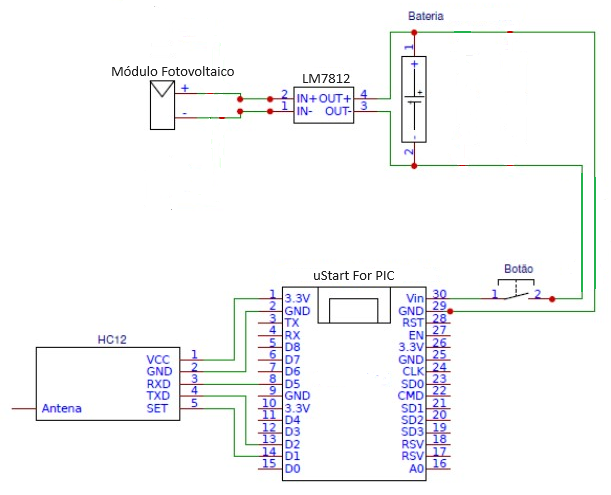
\includegraphics[width=10cm]{figuras/esquemaligac.png}\\
% 	\autoria{Autoria própria}
% 	\label{fig:ligac}
% \end{figure}

% Para garantir uma alimentação mais estável para o sistema, foi desenvolvido um módulo regulador de tensão, composto por um circuito integrado LM7812, que tem como função regular tensões entre 21V até 13V em uma tensão de 12V contínuos, foi inserido um capacitor de 100nF paralelo à saída do módulo para filtrar ruídos de alta frequência, o esquema de ligação do regulador é apresentado na Figura \ref{fig:reg}. Dessa forma, o sistema pode ser alimentado pelos módulos fotovoltaicos e bateria, como também por meio de uma fonte externa, ligada à tomada, como as usadas para carregar notebook.

% \begin{figure}[!h]
% 	\centering
% 	\caption{Esquema de ligação do regulador de tensão}
% 	%\vskip 5mm
% 	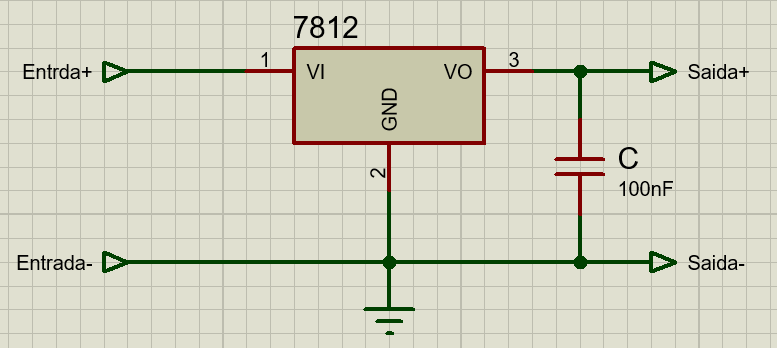
\includegraphics[width=10cm]{figuras/regulador.png}\\
% 	\autoria{Autoria própria}
% 	\label{fig:reg}
% \end{figure}

% Após a montagem física do circuito contendo módulo fotovoltaico de 15V, bateria de 12V, placa com PIC e os componentes que compõem o circuito de condicionamento de sinais, o protótipo é exibido na Figura \ref{fig:cond}.

% \begin{figure}[!h]
% 	\centering
% 	\caption{Módulo de condicionamento de sinais}
% 	%\vskip 5mm
% 	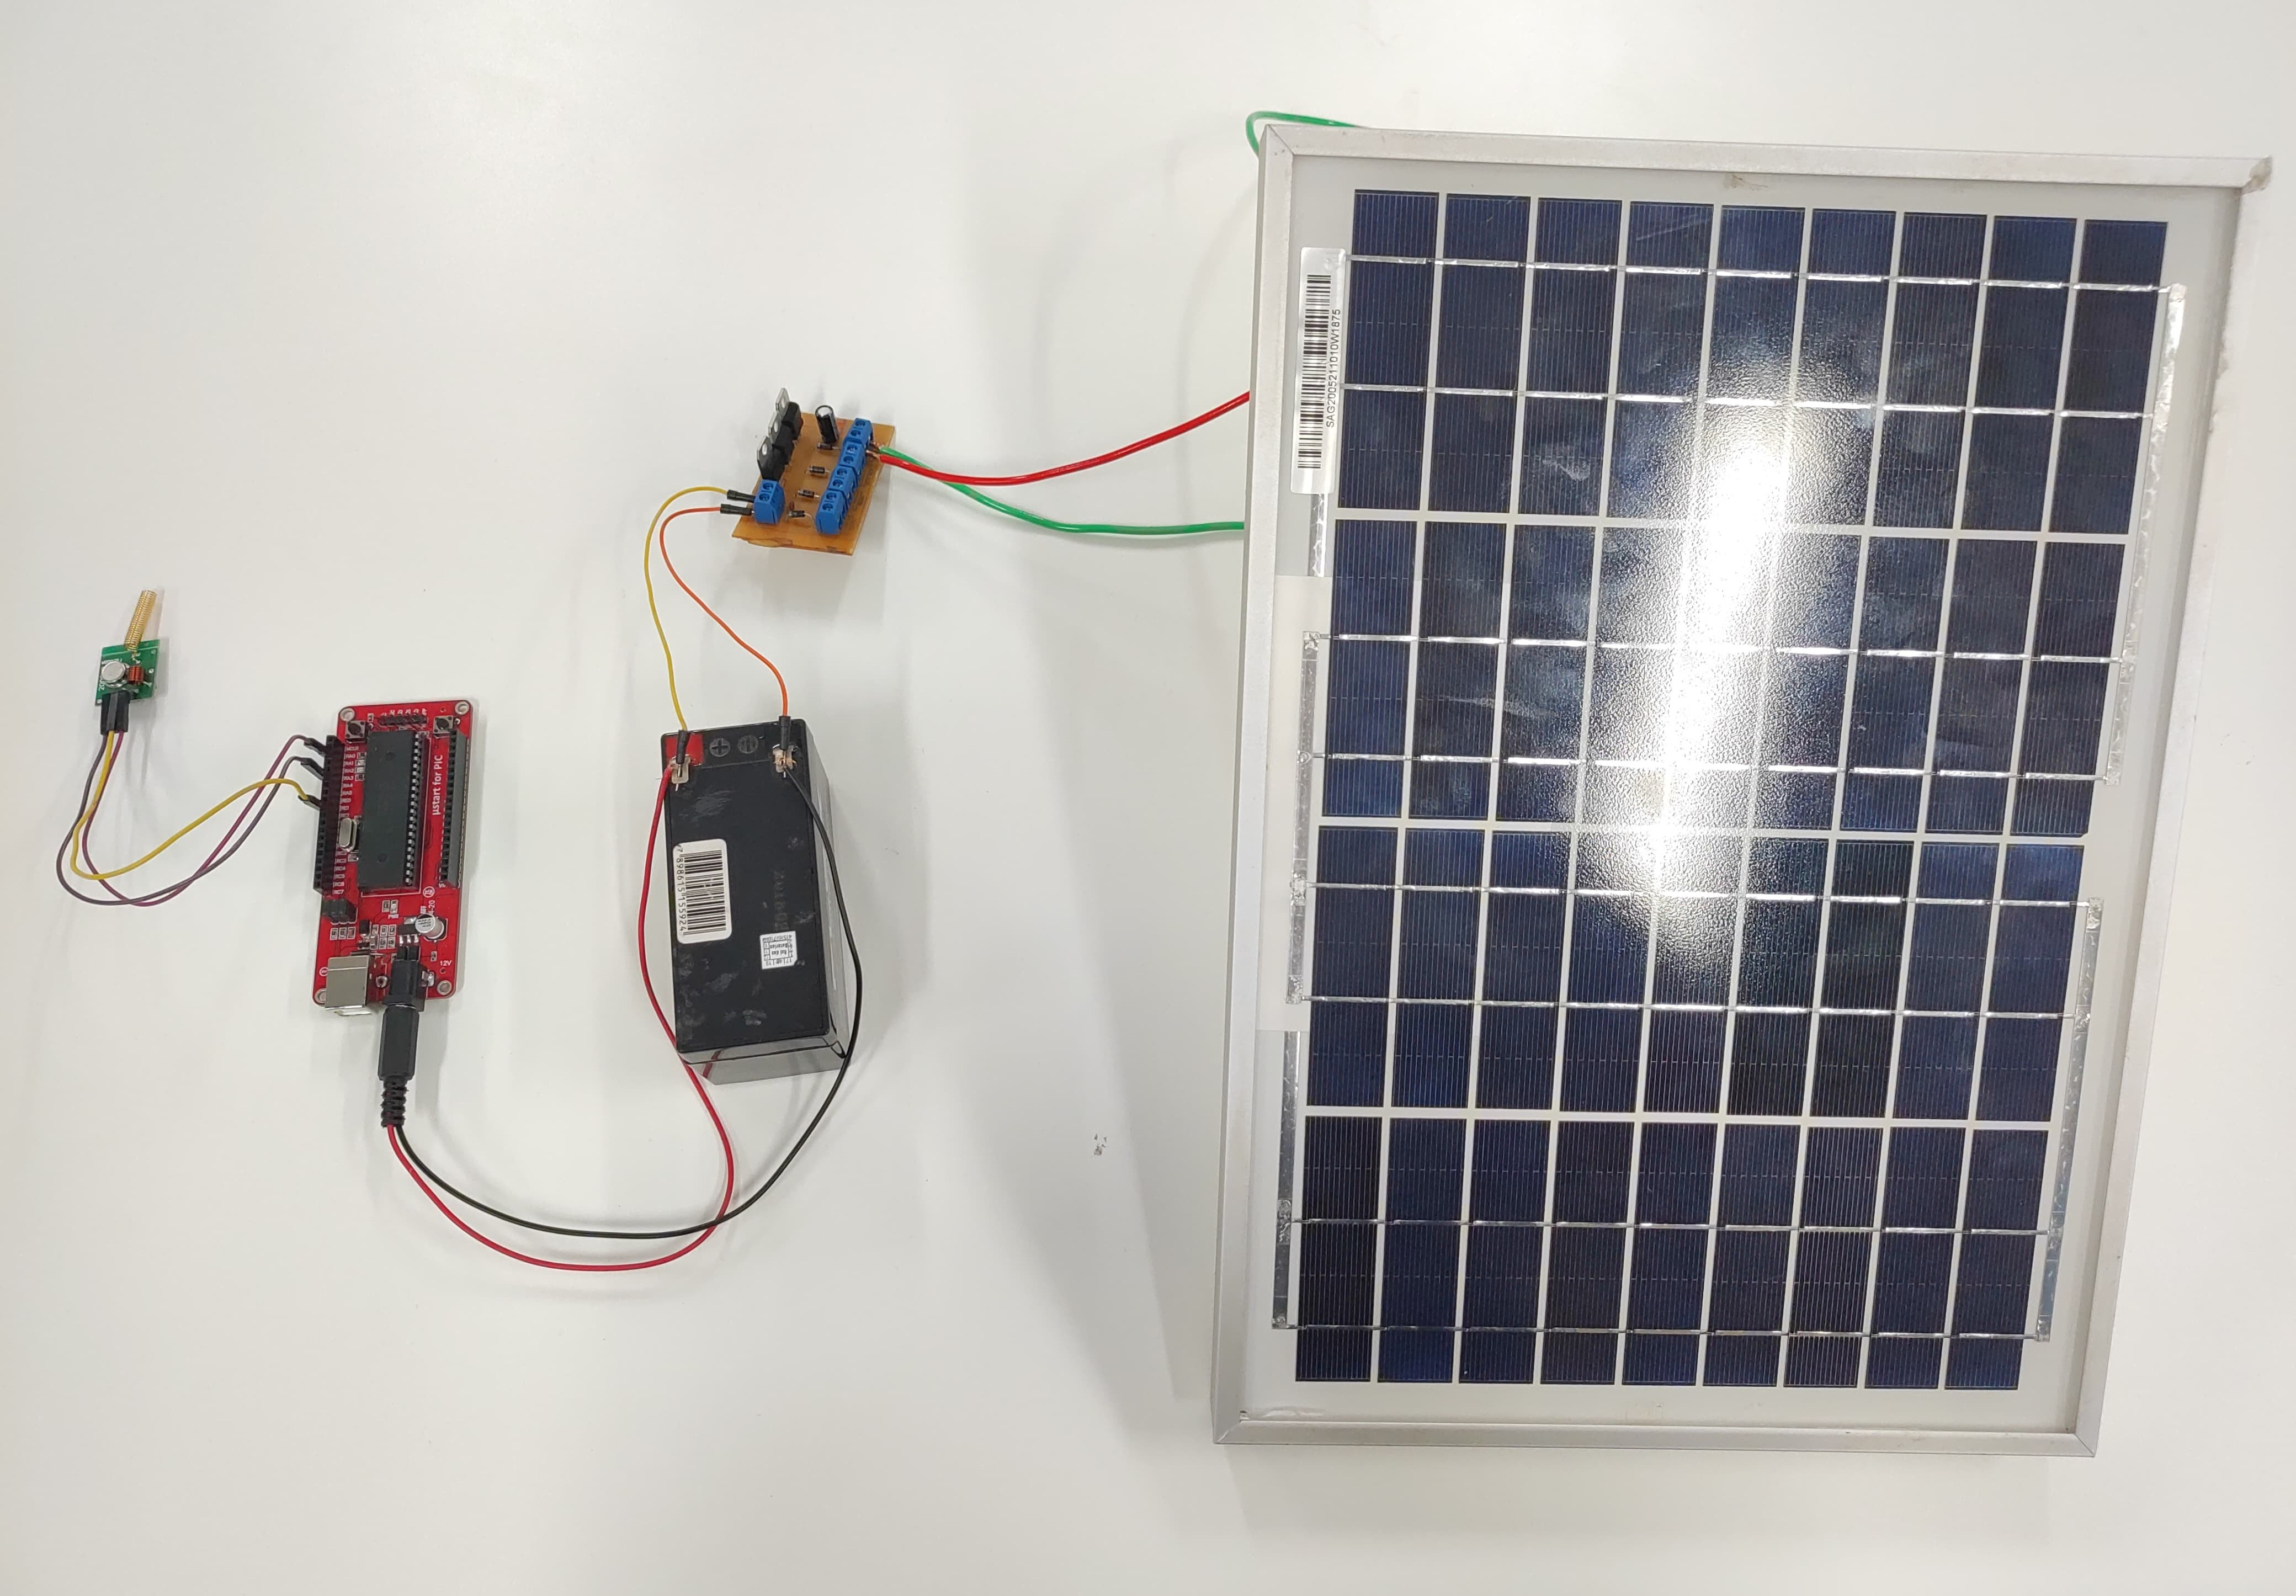
\includegraphics[width=10cm]{figuras/coisasmontadas.jpeg}\\
% 	\autoria{Autoria própria}
% 	\label{fig:cond}
% \end{figure}

% \subsection{Envio de dados}

% O envio de dados ocorre de diferentes maneiras entre os módulos. Entre os sensores, atuadores, interface Humano/Máquina física e circuito de condicionamento de sinais, os dados são enviados utilizando conexões físicas, por meio de cabos. A comunicação entre o circuito de condicionamento de sinais e o módulo central é realizada por radiofrequência utilizando dois módulos RF HC-12, que permitem uma conexão de até 6,5km entre os módulos. A troca de informações entre o módulo central e a interface Humano/Máquina virtual ocorre com o protocolo \ac{MQTT}.

% O protocolo MQTT foi implementado no ESP32, tendo esse a função de publicador principal, enviando os dados para o \textit{broker}. Foi utilizado um \textit{broker} gratuito chamado hivemq.com, de domínio público e utilizado para desenvolvimento de protótipos. Foi criado o tópico estufaautomatica/\textit{publisher}, onde serão publicados os dados enviados pelo ESP32 e os inscritos no tópico poderão receber esses dados. Dessa forma, foi inscrito no tópico a interface gráfica \textit{web}, que pode ser acessada por dispositivo conectado à internet.

% \subsection{Interface Humano/Máquina}

% A apresentação dos dados dos sensores e estados dos atuadores é realizada por meio de duas interfaces, sendo uma de maneira física conectada ao circuito de condicionamento de sinais, permitindo que funcione independentemente da conexão com o módulo central ou internet. A placa contem um visor onde são apresentados os dados dos sensores, LED's que indicam o estado dos atuadores, a existência de conexão com o módulo central e a indicação de placa energizada, e botões onde podem ser realizados teste de funcionamento dos atuadores e também a configuração e escolha do tipo de plantação a ser cultivada. Na Tabela \ref{tab:led} são apresentados as cores dos LED's e seus significados.

% \begin{table}[!h]
% \centering
% \caption{Descrição das cores}
% \label{tab:led}
% \begin{tabular}{c|c}
% \hline
% Cor do LED & Indicação \\ \hline
% Vermelho & Sistema energizado \\ \hline
% Azul & Comunicação com a IHM virtual \\ \hline
% Verde & Irrigação ativada \\ \hline
% Amarelo & Ventilação ativada \\ \hline
% \end{tabular}
% \\
% \autoria{Autoria própria}
% \end{table}

% A configuração do sistema ocorre de maneira simplificada, sedo acessível para pessoas com pouca afinidade com tecnologia. Para realizar a escolha da plantação, basta apertar o botão \textit{ENTER} a qualquer momento e entrar no menu de opções, em seguida pode-se navegar através dos botões para cima e para baixo, representados por setas, ao encontrar a opção desejada, aperta-se novamente o botão \textit{ENTER} e a escolha foi concluída.


% A interface foi desenvolvida em placa de circuito impresso para fornecer maior confiabilidade e resistência em suas conexões, além do posicionamento dos componentes oferecer simplicidade ao usuário, como pode ser visto na Figura \ref{fig:IHMP}.

% \begin{figure}[!h]
% 	\centering
% 	\caption{IHM física}
% 	%\vskip 5mm
% 	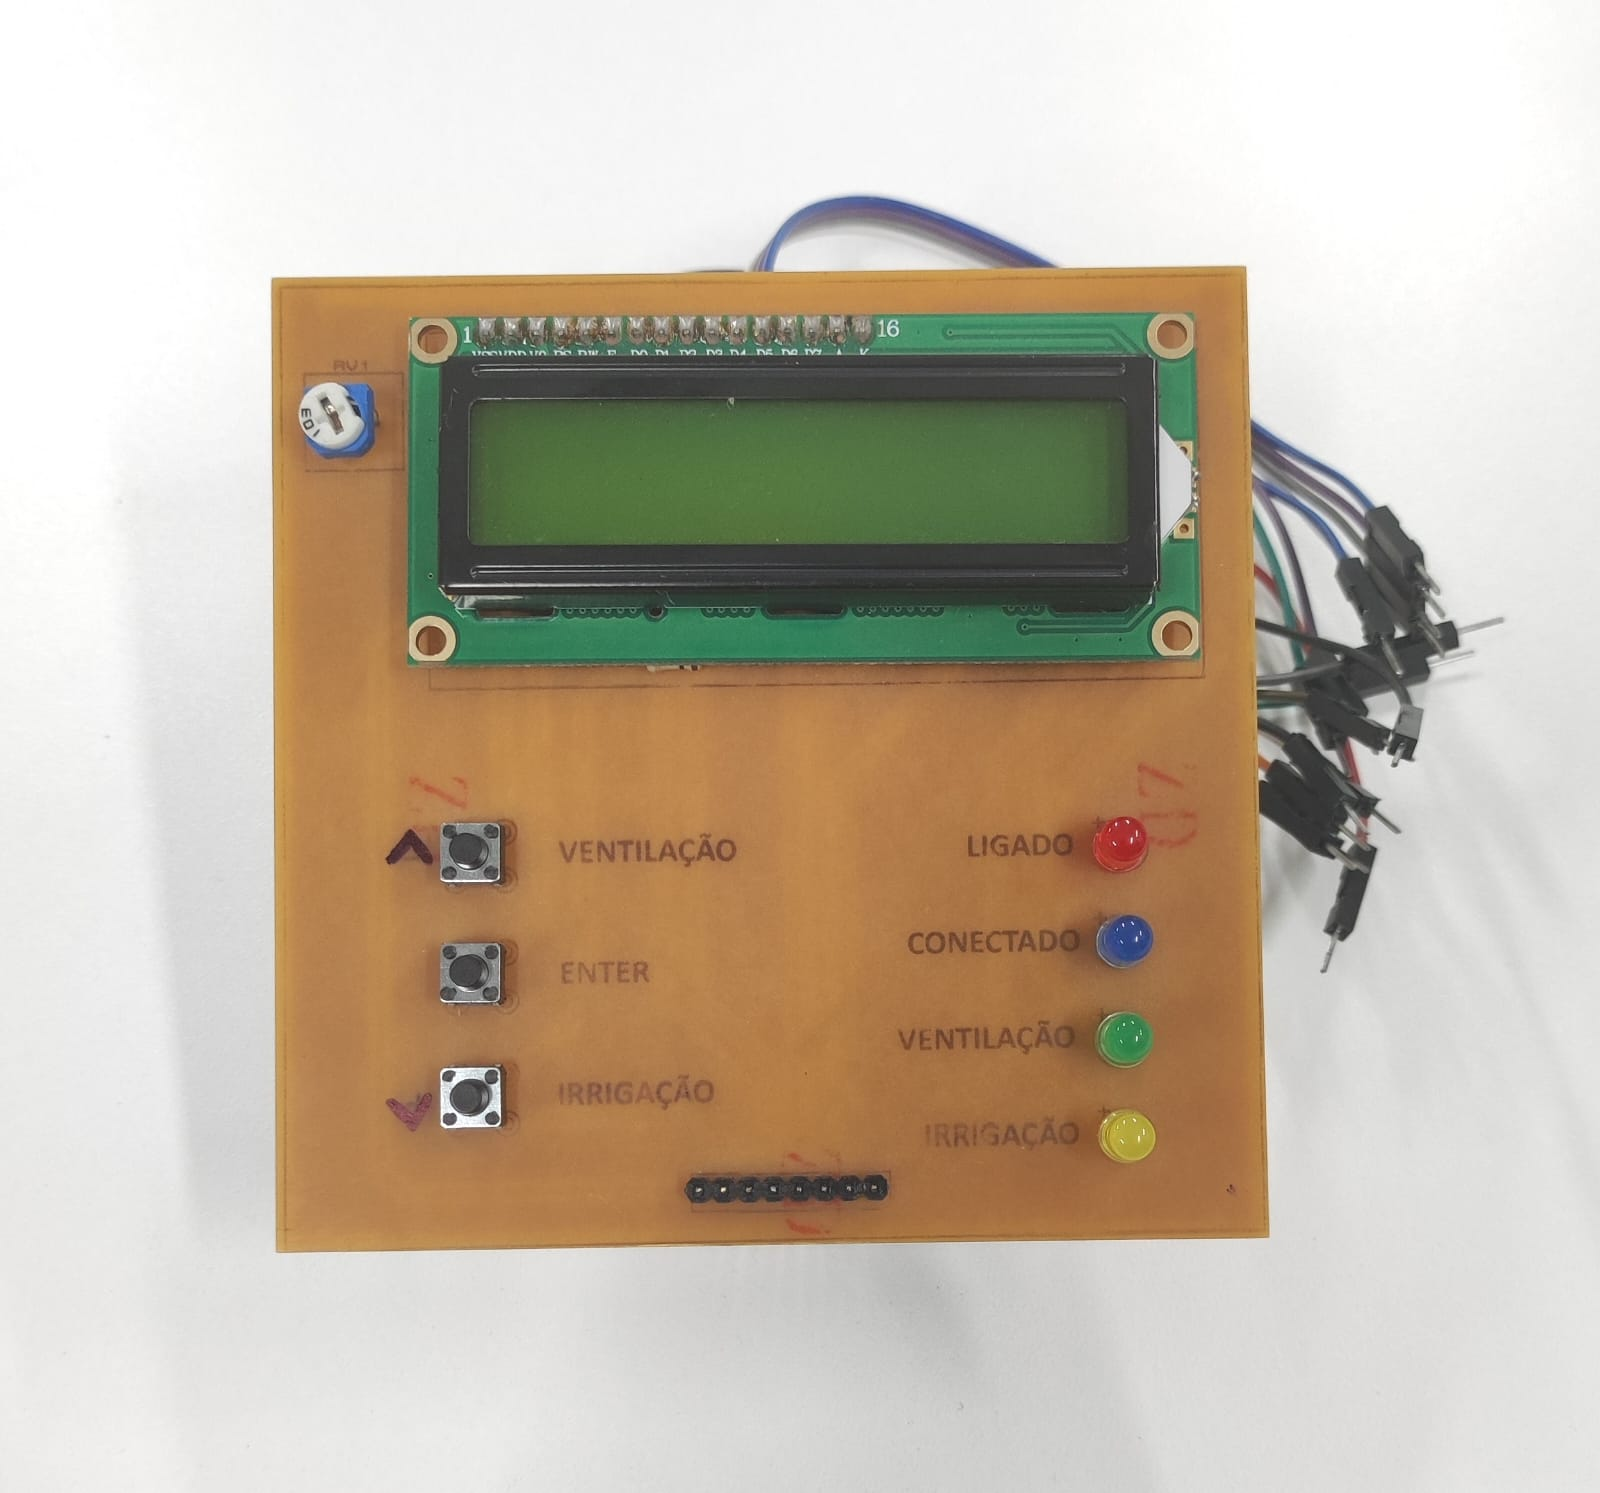
\includegraphics[width=10cm]{figuras/MINHAIHM.jpeg}\\
% 	\autoria{Autoria própria}
% 	\label{fig:IHMP}
% \end{figure}

% A interface gráfica que pode ser acessada por meio de computador ou celulares conectados à internet. Foi desenvolvido um aplicativo simples, usando a plataforma \textit{MIT App Inventor 2}, que fornece suporte para aplicações com protocolo MQTT. Essa plataforma permite o desenvolvimento de aplicativos usando programação em blocos simplificados, conforme Figura \ref{fig:progbloco}.

% \begin{figure}[!h]
% 	\centering
% 	\caption{Programação em blocos do aplicativo}
% 	%\vskip 5mm
% 	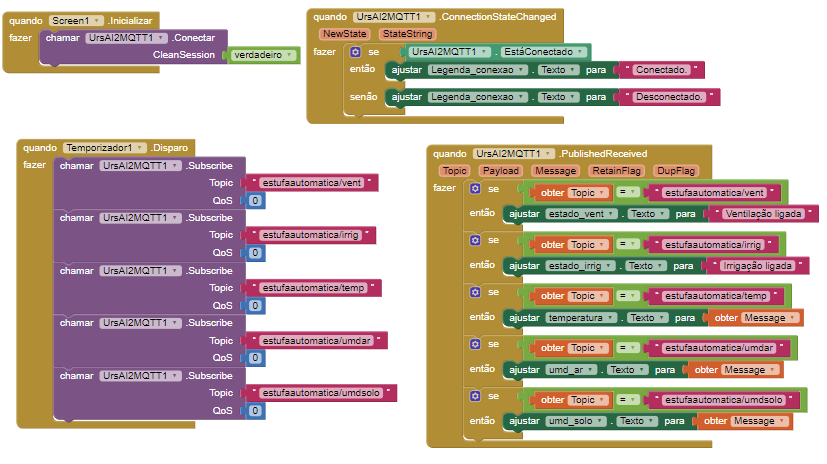
\includegraphics[width=12cm]{figuras/progbloco.png}\\
% 	\autoria{Autoria própria}
% 	\label{fig:progbloco}
% \end{figure}

% O aplicativo pode ser baixado gratuitamente pelo usuário através de link gerado durante o desenvolvimento do aplicativo, conforme mostrado na Figura \ref{fig:linkapk}. Foram adicionados na interface do aplicativo as mesmas informações que podem ser visualizadas pela interface humano/máquina física, no entanto, não permite realizar a configuração de escolha de plantio, sendo apenas possível ver a opção escolhida na IHM física. 

% \begin{figure}[!h]
% 	\centering
% 	\caption{Esquema de ligação do regulador de tensão}
% 	%\vskip 5mm
% 	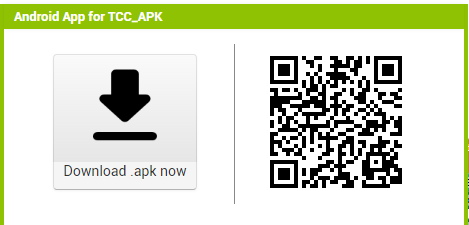
\includegraphics[width=12cm]{figuras/linkapk.png}\\
% 	\autoria{Autoria própria}
% 	\label{fig:linkapk}
% \end{figure}

% Conforme apresentado na Figura \ref{fig:apk}, o protótipo do aplicativo apresenta as principais informações do sistema de maneira simplificada, sendo de fácil manuseio e compreensão. 

% \begin{figure}[!h]
% 	\centering
% 	\caption{Interface do aplicativo de monitoramento}
% 	%\vskip 5mm
% 	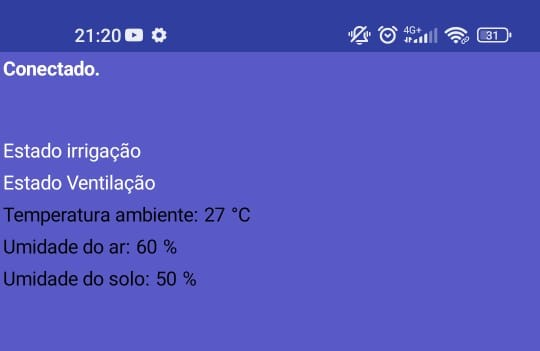
\includegraphics[width=10cm]{figuras/printapk.jpeg}\\
% 	\autoria{Autoria própria}
% 	\label{fig:apk}
% \end{figure}

% \subsection{Módulo central}

% O módulo central é responsável por intermediar a comunicação entre a \ac{IHM} e o circuito de condicionamento de sinais, tornando possível ao usuário o monitoramento remoto do sistema de irrigação, além de ser responsável por processar os comandos enviados pelo usuário. Esse módulo, apresentado na Figura \ref{fig:modcent}, é composto por placa ESP32, que faz a conexão com o servidor \ac{MQTT}, HC-12, que é utilizado para possibilitar a comunicação com o circuito de condicionamento. Esse módulo foi posicionado em localidade com acesso à internet, para possibilitar a conexão com a \ac{IHM}.

% \begin{figure}[!h]
% 	\centering
% 	\caption{Protótipo do módulo central}
% 	%\vskip 5mm
% 	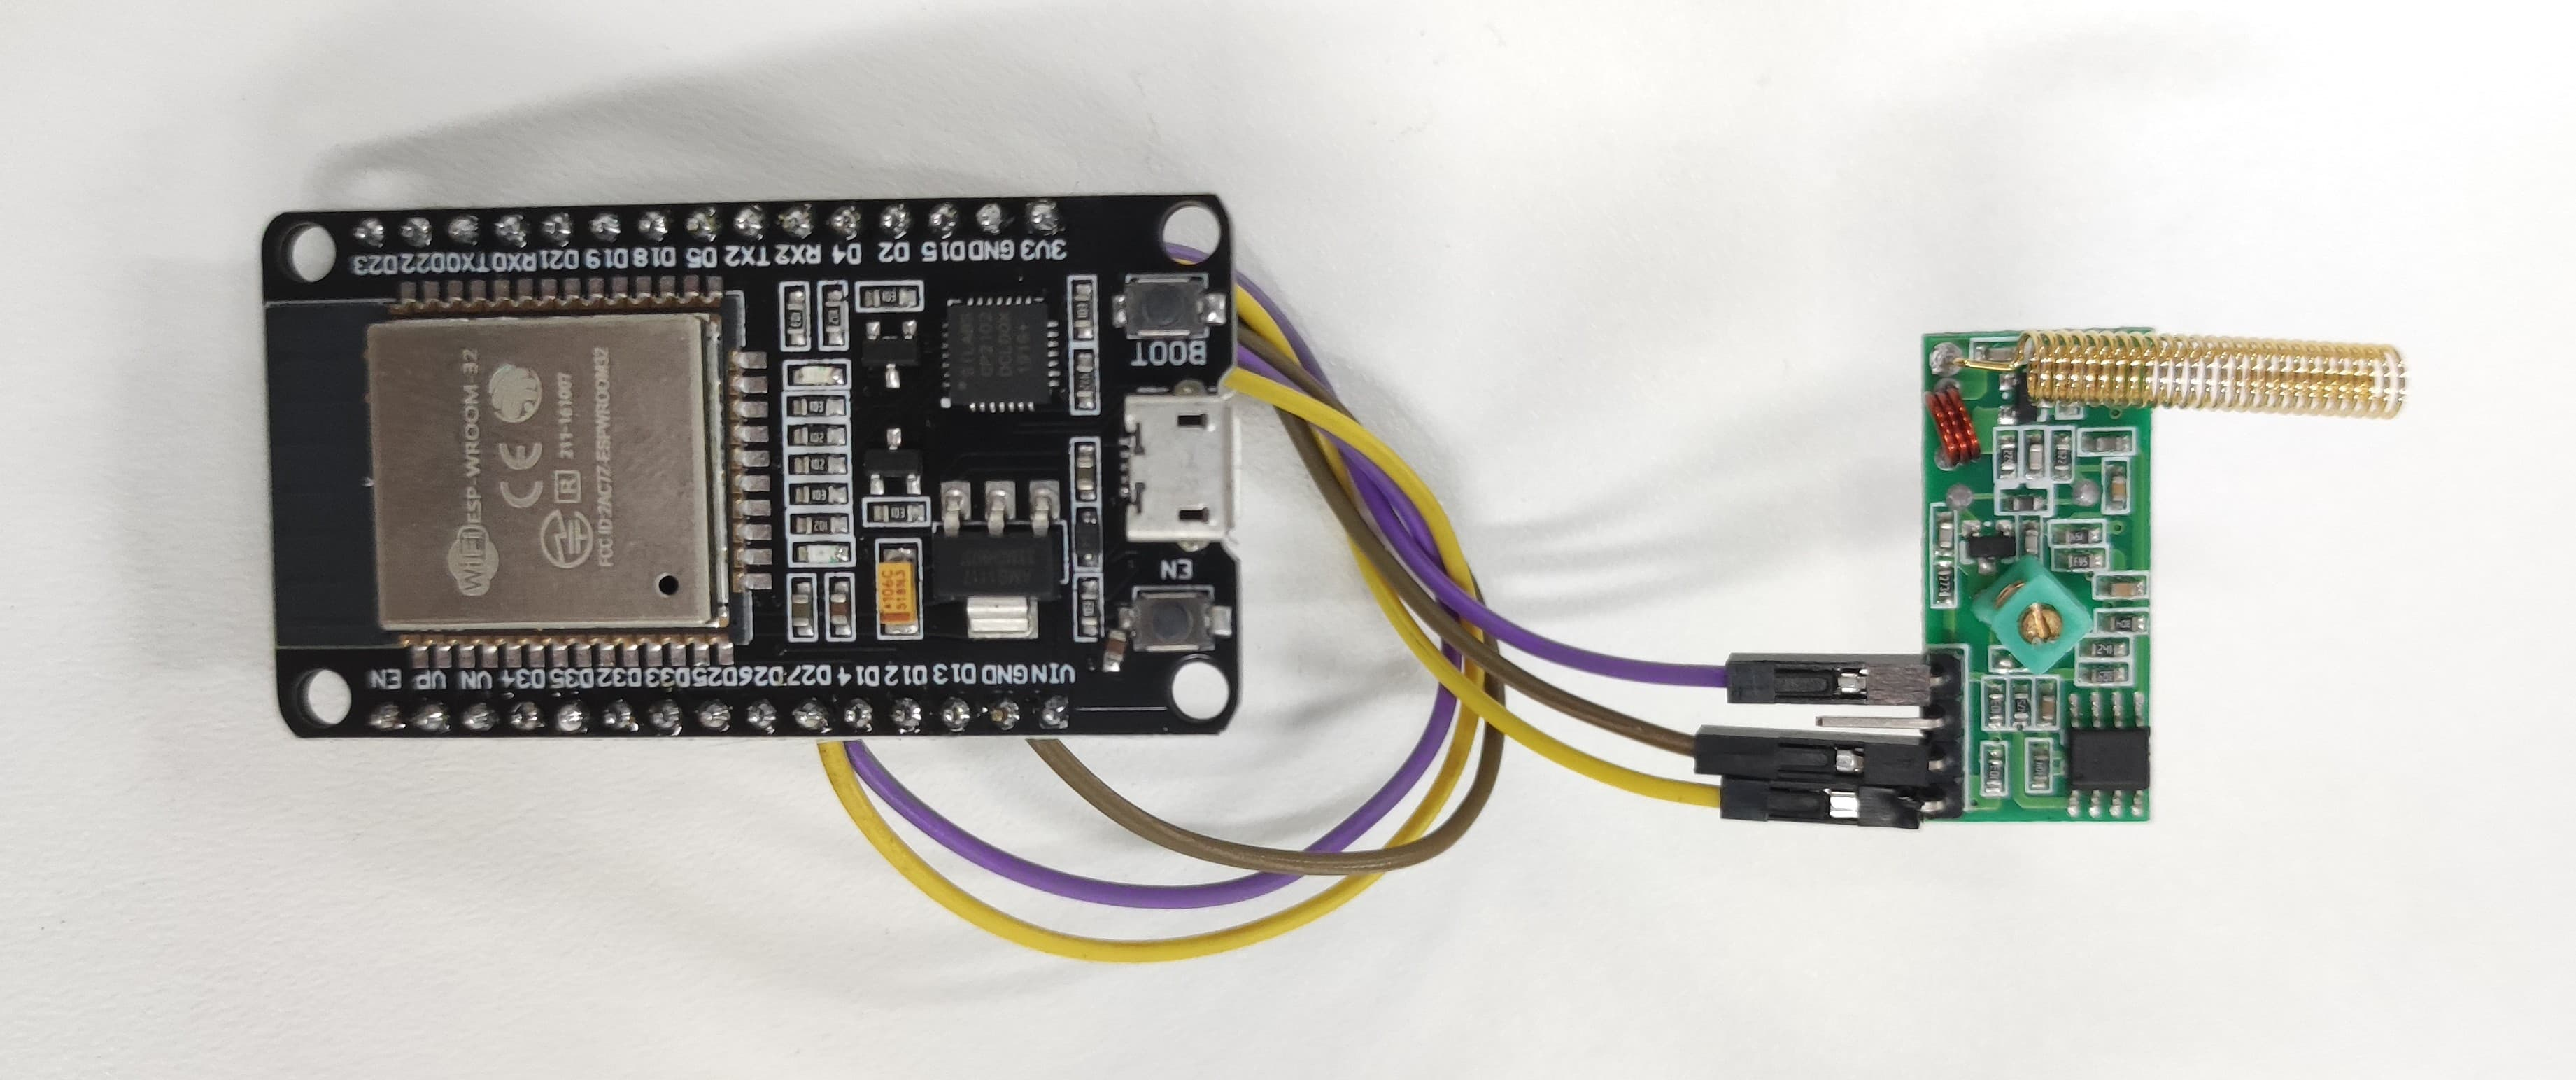
\includegraphics[width=10cm]{figuras/modcent.jpeg}\\
% 	\autoria{Autoria própria}
% 	\label{fig:modcent}
% \end{figure}

% \section{\textit{Software} embarcado}

% Neste trabalho, o \textit{Software} embarcado no microcontrolador foi desenvolvido com a linguagem C, utilizando a plataforma \textit{MikroC PRO for PIC} e a plataforma \textit{Arduíno IDE}. O fluxograma da Figura \ref{fig:alg} presenta de maneira simplificada o funcionamento da lógica de programação utilizada para o monitoramento e controle dos sistemas de ventilação e irrigação de uma estufa agrícola. 

% figura do fluxograma do software.
% \begin{figure}[!h]
% 	\centering
% 	\caption{Fluxograma do \textit{software} embarcado}
% 	%\vskip 5mm
% 	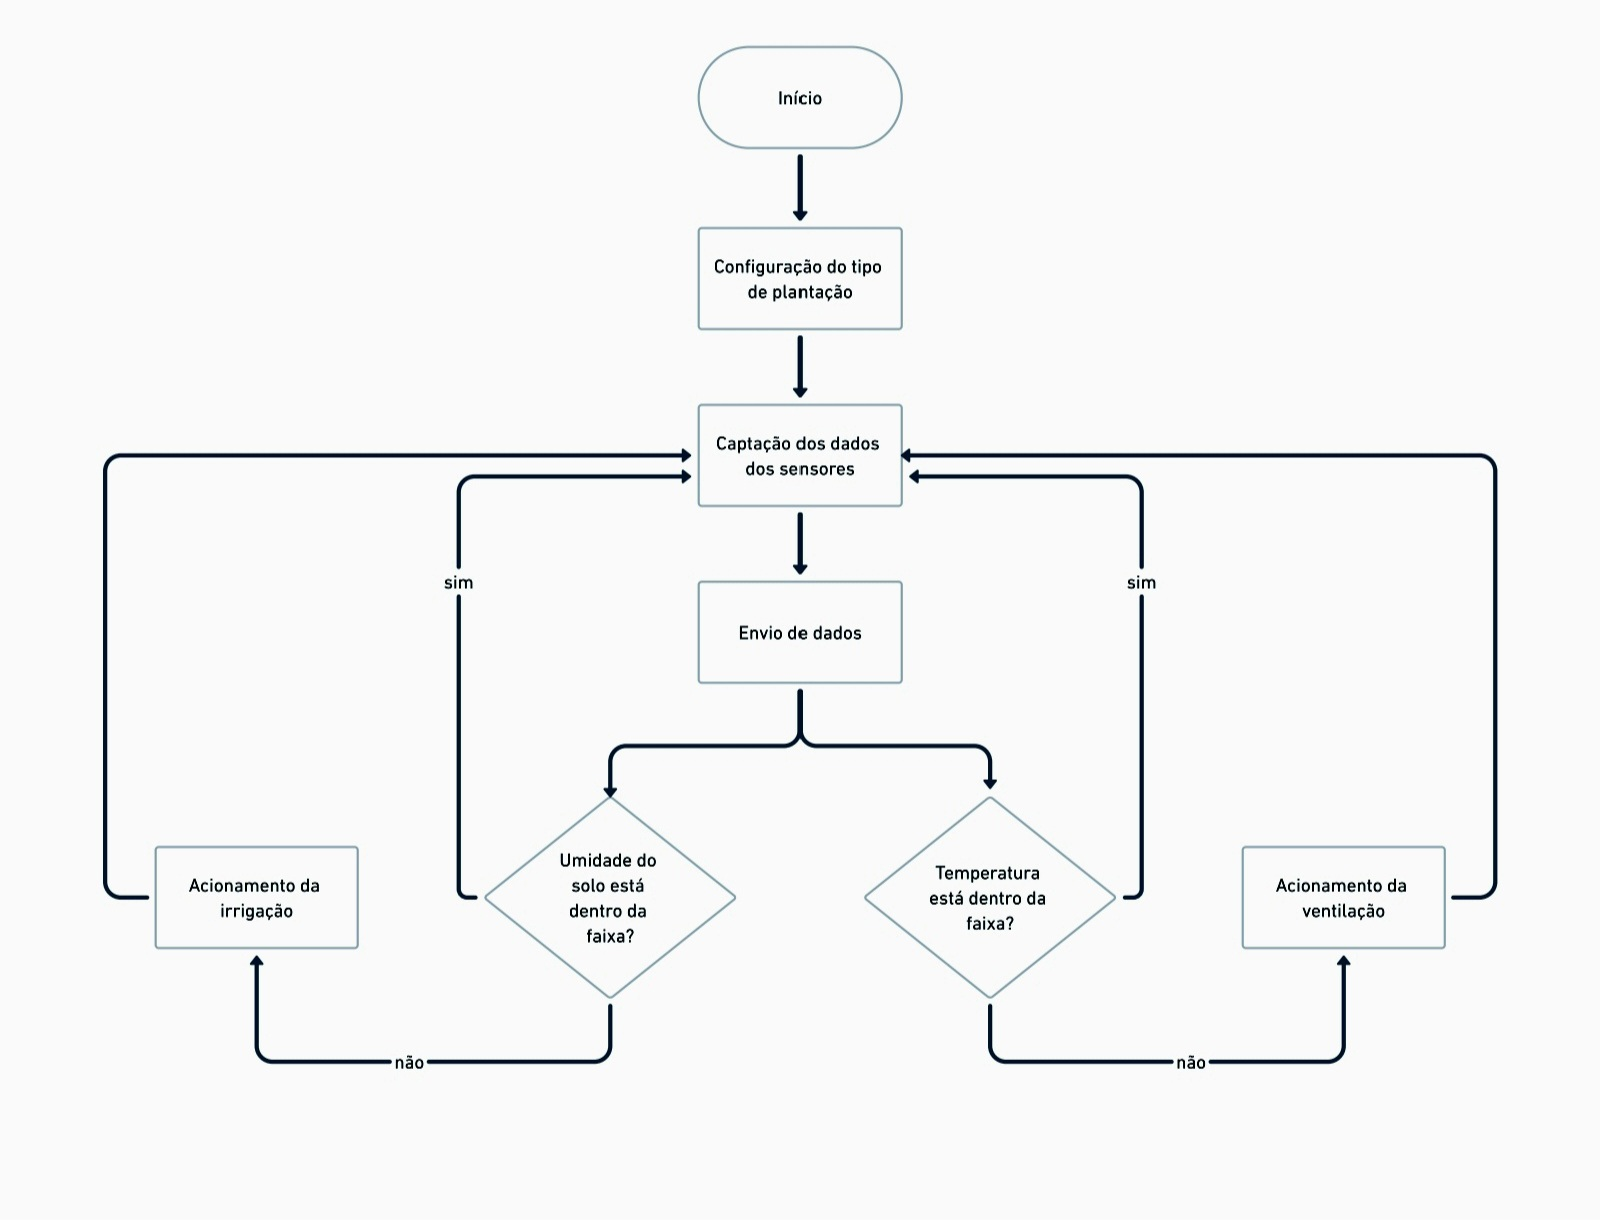
\includegraphics[width=12cm]{figuras/alg.jpg}\\
% 	\autoria{Autoria própria}
% 	\label{fig:alg}
% \end{figure}

% As principais etapas apresentadas no fluxograma são:
% \begin{enumerate}
%     \item Início: Inicializa o sistema com o carregamento das bibliotecas e a definição de variáveis e funções;
%     \item Configuração do tipo de plantação: Etapa em que o usuário escolhe o tipo de plantação que deseja aplicar o sistema, cada opção tem uma faixa de valores pré programados de temperatura e umidade do solo ideais para o plantio, essas faixas são informadas ao sistema após a escolha do usuário e passam a ser os parâmetros a serem alcançados pelo sistema;
%     \item Captação dos dados dos sensores: Nesta etapa o sistema coleta os dados dos sensores de umidade do solo, umidade relativa do ar e temperatura ambiente;
%     \item Envio de dados: Os dados coletados pelos sensores são enviados para a interface \textit{web}; 
%     \item Tomada de decisão: Caso o valor de temperatura ambiente não esteja dentro da faixa escolhida, a ventilação é acionada, os dados dos sensores são coletados novamente e uma nova tomada de decisão é realizada, o mesmo se aplica para a umidade do solo.
% \end{enumerate}   

% \subsection{Programação do sensor de temperatura e umidade do ar}

% O sensor DHT-22 possui uma programação complexa em comparação com outros sensores de temperatura, sendo dividida em funções que desempenham papeis diferentes em seu funcionamento, onde cada uma deve ser chamada no momento certo no código principal. Inicialmente foram definidas as portas onde o sensor foi conectado, em seguida foi definida a função de inicialização do sensor, chamada de \textit{start signal}, apresentada na Figura \ref{fig:startsig}.

% \begin{figure}[!h]
% 	\centering
% 	\caption{Função de inicialização do DHT-22}
% 	%\vskip 5mm
% 	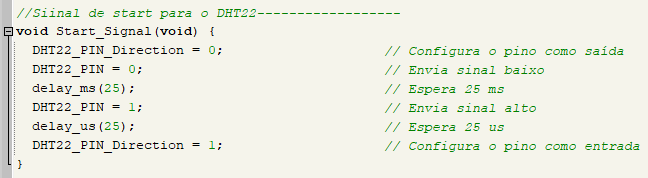
\includegraphics[width=12cm]{figuras/startsig.png}\\
% 	\autoria{Autoria própria}
% 	\label{fig:startsig}
% \end{figure}

% Essa função define o pino de conexão com o DHT-22 como saída e envia um pulso de nível lógico 1 por 20 ms, em seguida envia nível lógico 0 por 20ms, após isso o pino é definido como entrada e o sensor começa a enviar os dados. Em seguida, foi implementada a função que checa se a resposta do sensor apresenta algum erro, o código implementado é apresentado na Figura \ref{fig:chekres}. 

% \begin{figure}[!h]
% 	\centering
% 	\caption{Função de checagem da resposta do DHT-22}
% 	%\vskip 5mm
% 	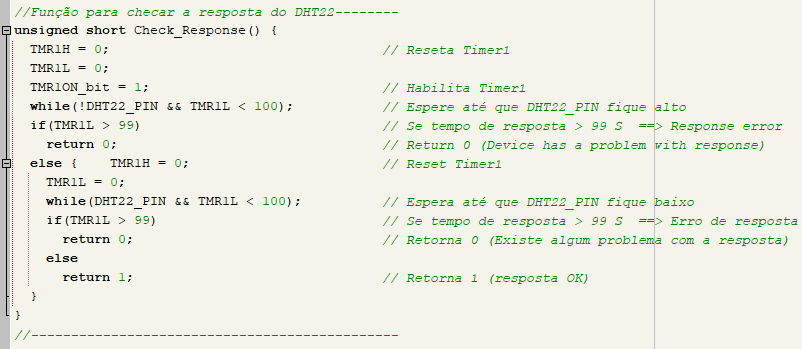
\includegraphics[width=12cm]{figuras/chekres.png}\\
% 	\autoria{Autoria própria}
% 	\label{fig:chekres}
% \end{figure}

% Essa função verifica a quantidade de bits recebidos do sensor e compara com o padrão de envio, que são 16 bits, caso encontre erro a função exibe a mensagem de erro na tela, caso contrario, da prosseguimento ao código. Seguindo para a função principal, ocorre a separação dos bits de umidade relativa do ar e os de temperatura ambiente, que são convertidos em valores decimais, que por sua vez, são usados para a tomada de decisão e exibidos ao usuário, conforme é visto na Figura \ref{fig:lerdados}.

% \begin{figure}[!h]
% 	\centering
% 	\caption{Função de leitura de dados do DHT-22}
% 	%\vskip 5mm
% 	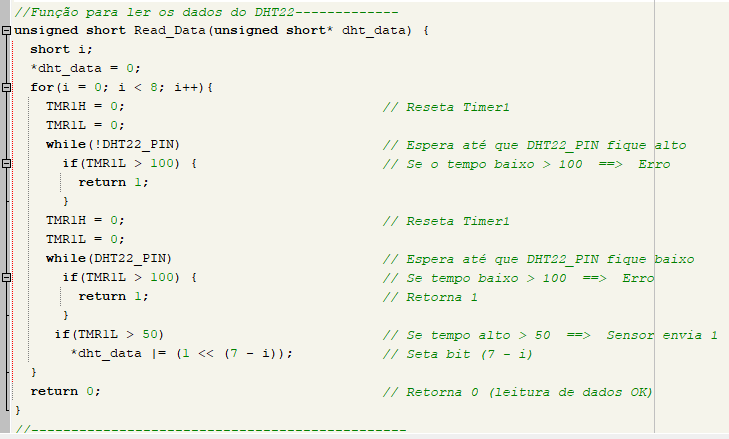
\includegraphics[width=12cm]{figuras/lerdados.png}\\
% 	\autoria{Autoria própria}
% 	\label{fig:lerdados}
% \end{figure}

% \subsection{Programação do sensor de umidade do solo}

% A programação referente ao sensor de umidade do solo é mais simples, visto que é enviado um valor analógico de tensão variando entre 0 a 5V, que é convertido pelo microcontrolador para um valor entre 0 a 1023, por conta do conversor analógico/digital do PIC18F4550 ser composto por 8 bits. Então, esse número é convertido para um valor entre 0 a 100\%, conforme apresentado na Figura \ref{fig:codsolo}, que corresponde à umidade do solo. 

% \begin{figure}[!h]
% 	\centering
% 	\caption{Função de leitura do sensor de umidade do solo}
% 	%\vskip 5mm
% 	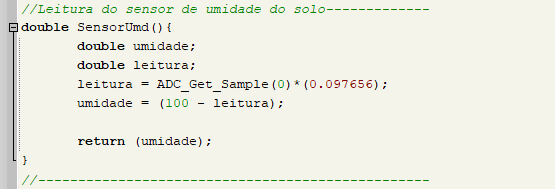
\includegraphics[width=12cm]{figuras/codsolo.png}\\
% 	\autoria{Autoria própria}
% 	\label{fig:codsolo}
% \end{figure}

% \subsection{Programação dos atuadores}

% Para o acionamento dos atuadores, foram desenvolvidas duas funções distintas, porém, com funcionamento parecidos. As funções recebem as faixas de valores ideais para o plantio escolhido pelo usuário, em seguida recebem os valores lidos pelos sensores. Para o acionamento da ventilação, a função compara os dados do sensor de temperatura com o valor programado, caso a temperatura esteja dentro da faixa, a função desliga a ventilação, caso esteja maior, a função liga a ventilação, conforme visto na Figura \ref{fig:codvent}.

% \begin{figure}[!h]
% 	\centering
% 	\caption{Função de acionamento da ventilação}
% 	%\vskip 5mm
% 	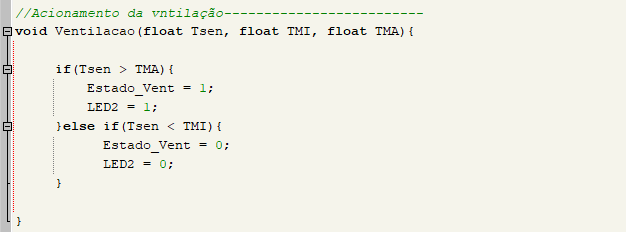
\includegraphics[width=12cm]{figuras/codvent.png}\\
% 	\autoria{Autoria própria}
% 	\label{fig:codvent}
% \end{figure}

% A função de acionamento da irrigação compara os dados do sensor de umidade do solo com a faixa de valores programados. Todavia, foi implementado um intervalo de histerese, para que não ocorra o acionamento e desacionamento desnecessário da irrigação, visto que os valores de umidade podem oscilar entre o limite do valor ideal conforme exibido na Figura \ref{fig:codirrig}.

% \begin{figure}[!h]
% 	\centering
% 	\caption{Função de acionamento da irrigação}
% 	%\vskip 5mm
% 	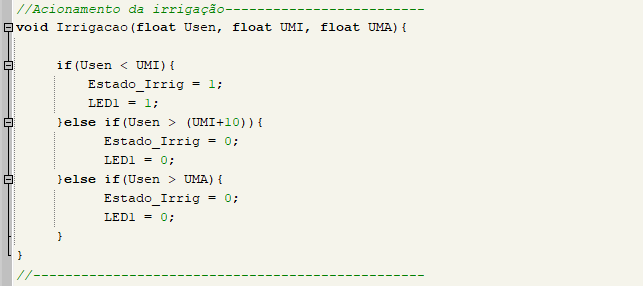
\includegraphics[width=12cm]{figuras/codirrig.png}\\
% 	\autoria{Autoria própria}
% 	\label{fig:codirrig}
% \end{figure}

% \section{Custo do sistema}

% O protótipo foi desenvolvido visando manter um custo baixo, em comparação aos produtos de automação de irrigação encontrados no mercado, para que possa ser acessível aos agricultores familiares e pequenos produtores. Desse modo, foram realizadas buscas pelos melhores preços para os componentes utilizados no projeto, a Tabela \ref{tab:custo} apresenta a relação de custo dos principais componentes do trabalho.

% \begin{table}[!h]
% \centering
% \caption{Custo do sistema}
% \label{tab:custo}
% \begin{tabular}{l|c|c|c}
% \hline
% Componente & \multicolumn{1}{l|}{Custo unitário (R\$)} & \multicolumn{1}{l|}{Quantidade (un)} & \multicolumn{1}{l}{Custo total (R\$)} \\ \hline
% Placa microStart & 60,00 & 1 & 60,00 \\ \hline
% Módulo Relé & 34,00 & 1 & 34,00 \\ \hline
% Esp32 & 38,90 & 1 & 22,90 \\ \hline
% Display LCD & 16,95 & 1 & 16,95 \\ \hline
% DHT-22 & 20,42 & 1 & 20,42 \\ \hline
% HD-38 & 9,32 & 1 & 9,32 \\ \hline
% HC-12 & 9,98 & 2 & 19,96 \\ \hline
% Insumos & 20,00 & 1 & 20,00 \\ \hline
% Caixa & 36,45 & 1 & 36,45 \\ \hline
% \textbf{Custo total} & - & - & \textbf{240,00} \\ \hline
% \end{tabular}
% \\
% \autoria{Autoria própria}
% \end{table}

% Insumos como resistores, diodos emissores de luz, botões, fios e cabos, placa de fenolite, capacitores e parafusos foram utilizados do próprio autor, sendo estimados em R\$ 20,00 reais. Por serem materiais com custo baixo em comparação aos principais componentes do sistema, essa estimativa não impacta significativamente na fidelidade do custo total do sistema implementado. 

% Foram realizadas pesquisas em lojas de agricultura na região de Irecê, para realizar uma comparação com um sistema comercial com características compatíveis com o protótipo, porém, apenas um sistema de automação de irrigação foi encontrado. O sistema não possui sensores de temperatura e umidade do solo, sendo controlado apenas válvulas solenoides para o controle de bombeamento de água, contando com divisão em diferentes setores. A programação a ser realizada também é mais complexa que o protótipo desenvolvido no presente trabalho, se tornando mais difícil de manusear, na Tabela \ref{tab:comp} é realizada uma comparação entre funcionalidades e custo do sistema comercial Irriplus VR e o sistema desenvolvido nesse trabalho.

% \begin{table}[!h]
% \centering
% \caption{Comparação entre os sistemas }
% \label{tab:comp}
% \begin{tabular}{l|c|c}
% \hline
% Funções & \begin{tabular}[c]{@{}c@{}}Protótipo \\ desenvolvido\end{tabular} & \begin{tabular}[c]{@{}c@{}}Irriplus \\ VR\end{tabular} \\ \hline
% \begin{tabular}[c]{@{}l@{}}Monitoramento de\\ temperatura\end{tabular} & SIM & NÃO \\ \hline
% \begin{tabular}[c]{@{}l@{}}Monitoramento de \\ umidade do ar\end{tabular} & SIM & NÃO \\ \hline
% \begin{tabular}[c]{@{}l@{}}Monitoramento de \\ umidade do solo\end{tabular} & SIM & NÃO \\ \hline
% Controle de irrigação & SIM & SIM \\ \hline
% Controle de ventilação & SIM & NÃO \\ \hline
% Divisão por setores & NÃO & SIM \\ \hline
% \begin{tabular}[c]{@{}l@{}}Monitoramento \\ remoto\end{tabular} & SIM & NÃO \\ \hline
% \textbf{Custo R\$} & 240,00 & 1529,86 \\ \hline
% \end{tabular}
% \\
% \autoria{Autoria própria}
% \end{table}

% Mesmo com custo quase seis vezes menor, o sistema desenvolvido se mostrou mais completo, tendo maior controle das variáveis que envolvem a irrigação, sendo uma boa opção para a agricultura familiar e também para grandes produtores.

% \section{Requisitos do sistema}

% Para determinar os requisitos que o trabalho deve atender, é necessário analisar os principais cultivos a serem implementados em estufas, buscando suas condições ideais de temperatura, umidade do solo e umidade relativa do ar. As cultivares predominantes em estufas são hortaliças, plantas hidropônicas e frutíferas, que apresentam necessidades semelhantes quanto ao clima, sendo possível estabelecer intervalos de valores que atendam a essas características.

% A temperatura ideal de cultivo de grande parte das plantas hidropônicas é de 25°C, para morangos e frutas semelhantes, é estabelecido um intervalo entre 15°C e 25°C para um bom desenvolvimento dos frutos, a temperatura ótima para e cultivo de cenouras e outras raízes tuberosas varia entre 20°C e 30°C. Com isso, compreende-se que o protótipo deve ser capaz de mensurar valores de temperatura compreendidos entre 15°C e 30°C para a maioria das plantações, contudo, para que o sistema possa quantificar também a variação de temperatura ambiente e com isso tomar melhores decisões de controle considerando a variação climática das diversas regiões do Brasil, a faixa de valores que deve ser medida compreende entre -15°C e 50°C.

% Para a umidade do solo os valores ideais dependem não apenas da variedade de cultivo, como também do tipo de solo. Contudo, a gama ideal de teor de umidade do solo para a maioria das culturas está entre 20\% e 60\%. É crucial para o bom funcionamento do sistema que o protótipo seja capaz de medir valores que estejam fora da faixa ideal de cultivo, para que o controle tome a decisão apropriada para a situação. Destarte, os valores a serem mensurados estarão entre 5\% e 95\%.

% Altos níveis de umidade relativa do ar geram condições favoráveis para o surgimento e proliferação de doenças nas plantas. Em contrapartida, níveis muito baixos podem ocasionar ressecamento no cultivo. A faixa a ser monitorada pelo sistema está compreendida entre 0 a 100\%. A Tabela \ref{tab:my-tablex} apresenta os valores a serem medidos como requisitos do sistema.

% \begin{table}[!h]
% \centering
% \caption{Parâmetros a serem medidos.
% }
% \label{tab:my-tablex}
% \begin{tabular}{c|c|c}
% \hline
% \textbf{Descrição}       & \textbf{Min}   & \textbf{Max}   \\ \hline
% {Temperatura}     & {-15°C} & {50°C}  \\ \hline
% {Umidade do solo} & {5\%}   & {95\%}  \\ \hline
% {Umidade do ar}   & {0\%}   & {100\%} \\ \hline
% \end{tabular}
% \\
% \autoria{Autoria própria}
% \end{table}

% %\section{Ferramentas computacionais utilizadas}



% \section{Metodologia de avaliação dos resultados}

% A avaliação dos resultados foi embasada nos objetivos do projeto e nos requisitos do sistema. Os módulos do sistema foram avaliados de acordo com a sua funcionalidade. Para o módulo de sensores foram avaliados a confiabilidade dos dados coletados, comparando-os com os valores reais, para isso foram realizados testes em ambiente controlado, para os atuadores foram verificados o tempo de resposta e a reação aos comandos enviados pelo módulo central.

% Para avaliar o envio de dados, foram levados em consideração a segurança da conectividade entre os módulos, além do alcance da conexão. Esses fatores são importantes para avaliar se o projeto é resistente à perdas de conexão e corrompimento dos dados transmitidos. Foram realizados testes variando-se a distancia entre os módulos, enviando dados conhecidos e comparando-os com a resposta obtida nos demais módulos. A \ac{IHM} deve ter uma interface amigável e intuitiva ao usuário, livre de erros de programação e travamentos. 






	\newpage \thispagestyle{empty}
	
	\chapter{RESULTADOS PARCIAIS}{}
\label{cap:05}
Nesta seção, serão apresentados os resultados parciais dos testes realizados, com foco na aplicação de uma rede neural convolucional para a classificação de doenças em plantações de bananeiras. O processo de treinamento e avaliação utilizou imagens do conjunto \ac{BananaLSD}, seguindo uma estratégia de validação cruzada. Esse método envolveu cinco ciclos de treinamento, nos quais as imagens processadas foram usadas para o treinamento, enquanto as imagens originais foram reservadas para os testes. Inicialmente, não foram empregadas técnicas de pré e pós-processamento.


\section{Sistema de Classificação}
Devido a quantidade de imagens e o limite computacional, a média de tempo para executar a tarefa de aprendizado é cerda de 4h e 30min. Outro fator que intefere na execução do custo computacional e tempo de processamento do algoritmo são os ajustes dos hiperparâmetros da rede neural projetada, uma vez que, o processo de treinamento é reiniciado.   

A estratégia utilizada na aplicação dos modelos citado no problema de classificação de doenças envolveu modificar os parametros de entrada, e analisar por meio de inspeção quais conjuntos de parâmetros se encaixa melhor.

A análise foi realizada com base em diversas métricas de desempenho, como acurácia, perdas e matriz de confusão, permitindo uma avaliação abrangente do sistema. Esses indicadores servem para uma compreensão melhor e mais detalhada dos resultados obtidos. 

\subsection{Avaliação de Desempenho do Sistema de Classificação}
Foram realizados  o treinamento ao longo de 10 épocas utilizando os valores iniciais, conforme ilustrado na Figura \ref{Fig:10epocas}. Os hiperparâmetros selecionados para este experimento incluem um tamanho de lote de 80 e uma taxa de aprendizado de $0,0001$. Os  gráficos apresentam tanto o erro quanto a acurácia. No gráfico de erro, é possível notar uma queda progressiva, indicando que o aprendizado está ocorrendo ao longo do treinamento, neste caso, está de acordo com as expectativas para o modelo. Porem, o gráfico de acurácia não apresenta uma melhoria tão grande. Esse resultado possivelmente está relacionado ao pequeno número de épocas ou um pequeno desvio nos parametros, fazendo com que o modelo não atinja a performance esperada. 

\begin{figure}[!h]
	\centering
	\caption{Treinamento ao longo de 10 épocas.}
	%\vskip 5mm
	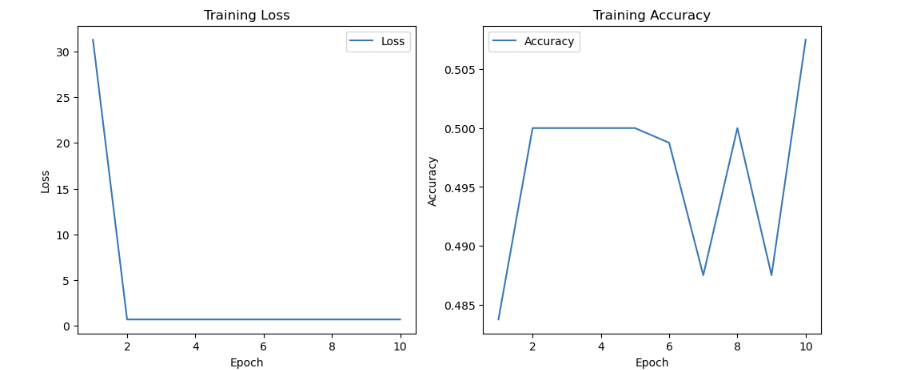
\includegraphics[width=15cm]{figuras/10 epocas.png}\\
	\autoria{Autoria Própria (2024)}
	\label{Fig:10epocas}
\end{figure}

Na Figura \ref{Fig:50epocas}, o treinamento foi realizado ao longo de 50 épocas com hiperparâmetros ajustados: tamanho do lote de 96 e taxa de aprendizado de 0,0005. Nesse experimento, observou-se uma melhora no desempenho em relação ao primeiro teste. O gráfico de erro apresentou uma diminuição mais acentuada, indicando que o modelo estava aprendendo de forma mais eficiente. O gráfico de acurácia também mostrou um aumento gradual, embora os valores ainda não tenham alcançado níveis desejáveis.

\begin{figure}[!h]
	\centering
	\caption{Treinamento ao longo de 50 épocas.}
	%\vskip 5mm
	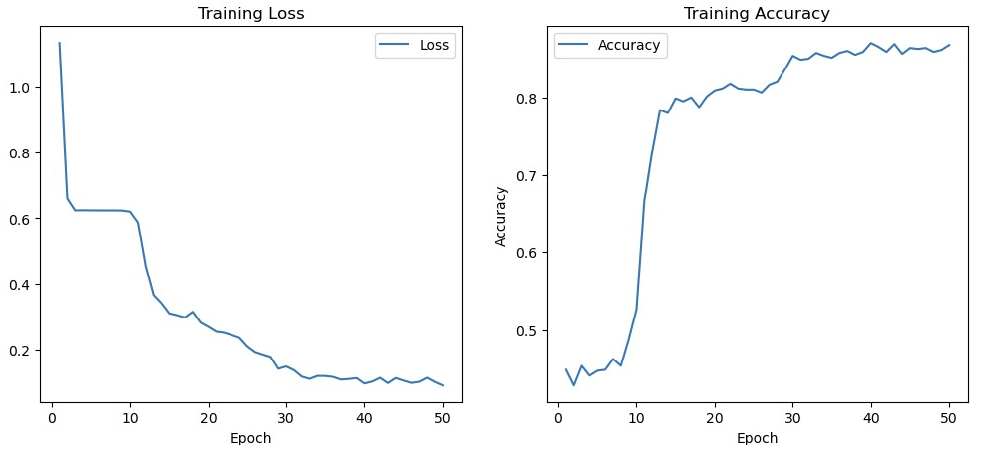
\includegraphics[width=14.4cm]{figuras/50 epocas.png}\\
	\autoria{Autoria Própria (2024)}
	\label{Fig:50epocas}
\end{figure}

Por fim, a Figura \ref{Fig:100epocas} apresenta o desempenho do modelo otimizado, treinado ao longo de 100 épocas. Os hiperparâmetros ajustados para este experimento foram um tamanho de lote de 120 e uma taxa de aprendizado de 0,0005. Com essas configurações, o modelo alcançou uma melhoria significativa em comparação aos experimentos anteriores. O gráfico de erro demonstrou uma redução contínua e mais pronunciada, indicando uma maior eficiência no ajuste do modelo aos dados. O gráfico de acurácia revelou um aumento consistente, com a acurácia final atingindo níveis bastante satisfatórios.


\begin{figure}[!h]
	\centering
	\caption{Treinamento ao longo de 100 épocas.}
	%\vskip 5mm
	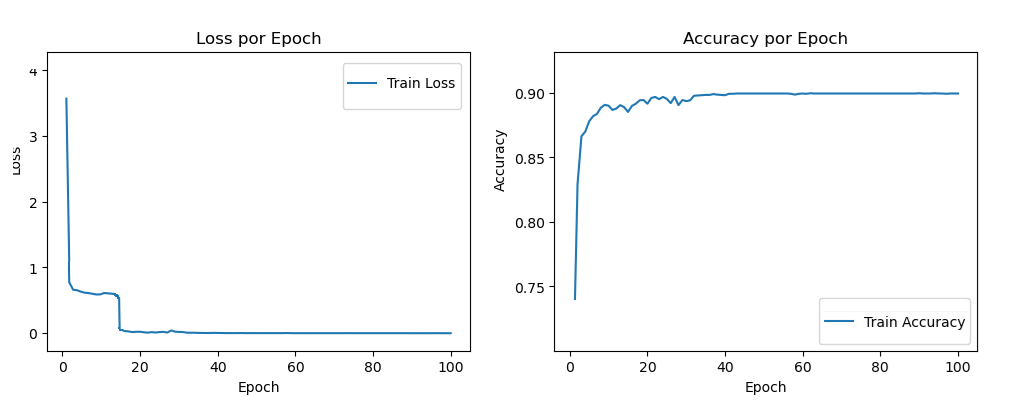
\includegraphics[width=15cm]{figuras/100 epocas.png}\\
	\autoria{Autoria Própria (2024)}
	\label{Fig:100epocas}
\end{figure}

 A \ac{MC} da Figura \ref{Fig:100Matriz} demonstra o desempenho do melhor modelo de classificação, apresentando a distribuição dos casos de verdadeiros e falsos positivos e negativos. O quadrante superior esquerdo indica que o modelo classificou corretamente 235 casos de SIGATOKA, enquanto o quadrante superior direito indica que classificou incorretamente 165 casos. No quadrante inferior esquerdo, estão os casos de falso positivo, ou seja, o modelo classificou incorretamente 18 imagens saudáveis como SIGATOKA. Por fim, no quadrante inferior direito, o modelo classificou corretamente 382 casos de folhas saudáveis.

Analisando a matriz de confusão, é possível notar que o modelo apresenta um bom desempenho. Caso contrário, é mais fácil identificar quais classes estão apresentando dificuldades, permitindo ajustar os hiperparâmetros ou explorar estratégias para melhorar a performance geral do modelo.

 
No entanto, é necessário resaltar que o desafio se dar pela demora no processo de aprendizado. Cada ajuste nos parâmetros exige um tempo considerável para completar novamente o treinamento, sendo que, o resultado de cada iteração leva por cerca de 3 horas. Isso pode tornar o processo de otimização lento e custoso, especialmente quando são necessários múltiplos testes.

\begin{figure}[!h]
	\centering
	\caption{Matriz de confusão}
	%\vskip 5mm
	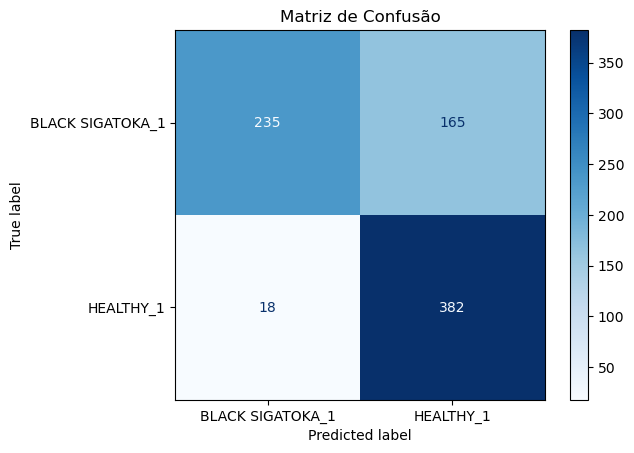
\includegraphics[width=10cm]{figuras/100 epocMatriz.png}\\
	\autoria{Autoria Própria (2024)}
	\label{Fig:100Matriz}
\end{figure}


\section{CONSIDERAÇÕES FINAIS E CRONOGRAMA}

O sistema proposto neste trabalho busca identificar problemas na plantação de bananeiras. Dessa forma, foi projetado um classificador baseado eme redes neurais convolucionais para processamento de imagens e detecção de doenças na cultura avaliada. Inicialmente,  projetou-se um classificador binário (apenas duas classes), em que considerou-se a folha da bananeira sem a doença e com a sigatoka (considerada a doença mais destrutiva da cultura da bananeira). Resultados encontrados mostraram-se promissores, embora, apresente necessidades de ajustes no sistema projetado a fim de otimizar os resultados de classificação. Assim, para etapa seguinte, pretende-se utilizar etapas de pré e pró processamento, além de avaliar outras doenças, gerando um classificador de multiplas classes. 

Neste contexto, para dar continuidade ao trabalho deve-se desenvolver as atividades previstas no quadro~\ref{tab:q2}, distribuídas conforme complexidade, eventos e tempo necessário para conclusão de cada etapa, e assim finalizando o trabalho. 


%colocar a tabela na página de cima
\begin{quadro}[!htb]
%\caption{Principais referências bibliográficas consultadas} \label{tab:q1}\\
\caption{Cronograma das atividades que serão realizadas durante o projeto.}\label{tab:q2}
\centering
\begin{tabular}{|p{45 mm }|c|c|c|c|c|c|}

\hline \centering \textbf{\footnotesize Atividades Previstas}   & \textbf{\footnotesize Out}  & \textbf{\footnotesize Nov} & \textbf{\footnotesize Dez} & \textbf{\footnotesize Jan} & \textbf{\footnotesize Fev} & \textbf{\footnotesize Mar} \\
\hline  Revisão bibliográfica&   x & x &  &  & &    \\ 
\hline  Preparar mais dados para inspeção & x & x  &  &  &  &   \\ 
\hline Ajustar a rede neural para novas doenças;  &   &  x &  &  &  &\\ 
\hline  Treinamento a rede neural convolucional;   &  &  & x & x &  &  \\
\hline  Identificar doenças do cultivo da banana   &  &  & x & x &  &  \\ 
\hline Analisar a acurácia e a taxa de erro da rede neural;     &  &  &  & x & x &    \\ 
%\hline Fazer a avaliação dos dados obtidos durante o experimento   &  &  & x & x &    \\  
\hline  Redigir TCC   &  &  &  & x & x & x  \\
\hline  Defender TCC   &  &  &  &  &  & x  \\
\hline 
\end{tabular}
\end{quadro}


% Nesta seção serão apresentados os resultados dos testes para validação do trabalho. Cada módulo do sistema foi testado separadamente, de acordo com sua funcionalidade, em seguida foram realizados testes do sistema funcionado integralmente, aplicado ao protótipo de estufa. 


% \section{Módulo sensores}

% Para validar o módulo de sensores, foram realizados testes específicos para cada grandeza medida pelos sensores. Foram testados valores compreendidos na Tabela \ref{tab:my-tablex}, objetivando-se alcançar os extremos de cada grandeza. 

% \subsection{Testes de temperatura}

% Com o sensor de temperatura conectado ao circuito de condicionamento de sinais, foram realizados testes em laboratório. Foram medidos valores e comparados com medidas realizadas com termômetro digital. A primeira medida foi realizada em um congelador, onde foi possível constatar que o sensor é capaz de aferir temperaturas negativas. Foram realizados testes à temperatura ambiente, como apresentado na Figura \ref{fig:testetemp}, onde o valor coincidiu com o termostato do controle do ar-condicionado.

% \begin{figure}[!h]
% 	\centering
% 	\caption{Estado da bomba submersa}
% 	%\vskip 5mm
% 	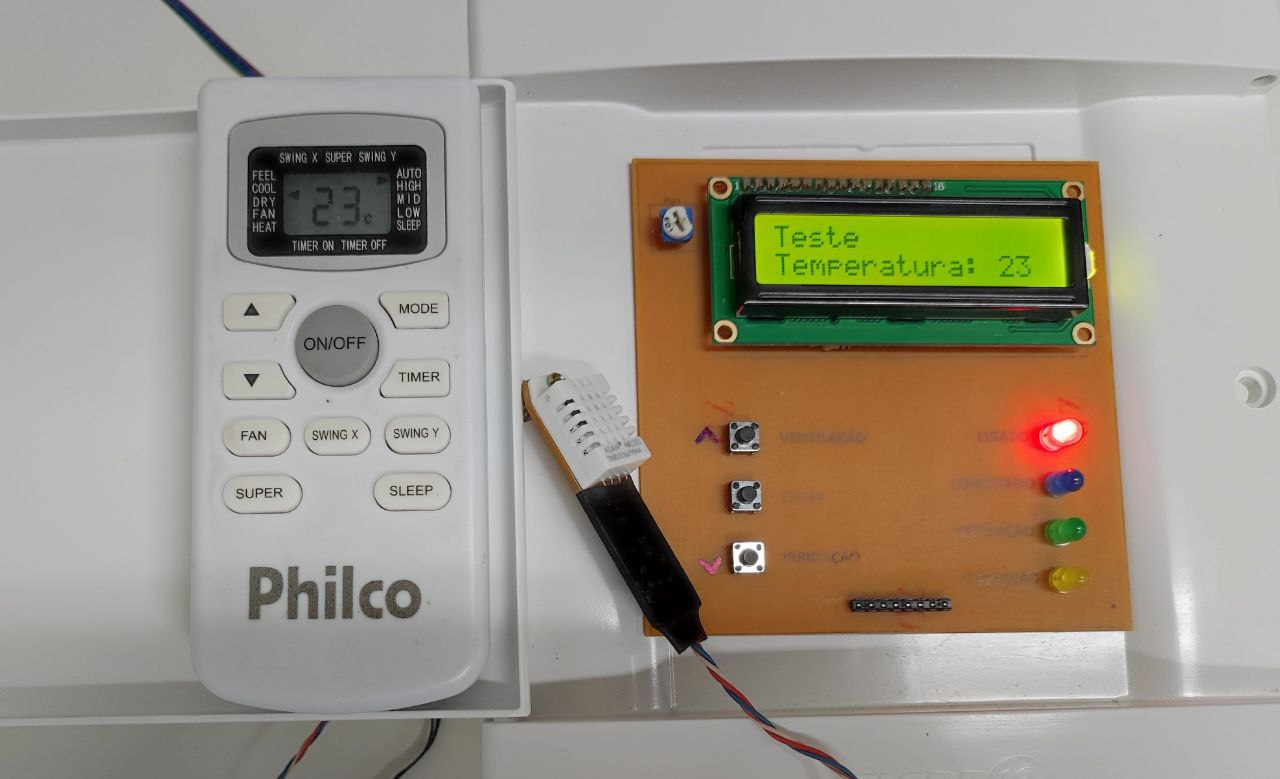
\includegraphics[width=12cm]{figuras/testetemp.jpg}\\
% 	\autoria{Autoria Própria}
% 	\label{fig:testetemp}
% \end{figure}

% Foram realizados testes em outros ambientes, resultando em dados aproximados da temperatura real. Dessa forma, o sensor DHT-22 apresentou resultados satisfatórios e condizentes com a aplicação, com suas variações estando dentro da faixa estabelecida na folha de dados do sensor.

% \subsection{Testes de umidade do ar}

% Por se tratar de uma grandeza difícil de controlar com os recursos presentes, foram realizados apenas teste de umidade relativa do ar em ambiente externo e interno, realizando múltiplas medidas e comparando a variação entre elas. A Tabela apresenta os resultados das medidas obtidas nos testes.

% \begin{table}[!h]
% \centering
% \caption{Medidas de umidade do ar em ambiente interno e externo}
% \label{tab:umidadear}
% \begin{tabular}{c|c|c}
% \hline
% Umidade do ar & Ambiente interno & Ambiente externo \\ \hline
% Medida 1 & 38.9\% & 34.7\% \\ \hline
% Medida 2 & 38.9\% & 34.6\% \\ \hline
% Medida 3 & 39.6\% & 34.7\% \\ \hline
% Medida 4 & 39.4\% & 35.2\% \\ \hline
% Medida 5 & 39.6\% & 35.3\% \\ \hline
% \end{tabular}
% \\
% \autoria{Autoria própria}
% \end{table}

% Analisando os dados apresentados, é possível observar uma baixa variação entre os valores de umidade relativa do ar, sendo a umidade medida em ambiente interno ligeiramente maior, por conta da presença de pessoas no local e baixa ventilação. Por conta da constância dos resultados, é possível afirmar que a confiabilidade do sensor está condizente com os requisitos do sistema. 

% \subsection{Testes de umidade do solo}
% Os testes de umidade do solo foram realizados em recipientes contendo variados tipos de terra e variando a quantidade de água presente. Primeiramente foi medido o valor obtido pelo sensor sem contato com o solo, como visto na Figura \ref{fig:avazio}. O valor esperado para o teste era de 0\%, sento obtido medida equivalente.

% \begin{figure}[!h]
% 	\centering
% 	\caption{Teste com sensor seco}
% 	%\vskip 5mm
% 	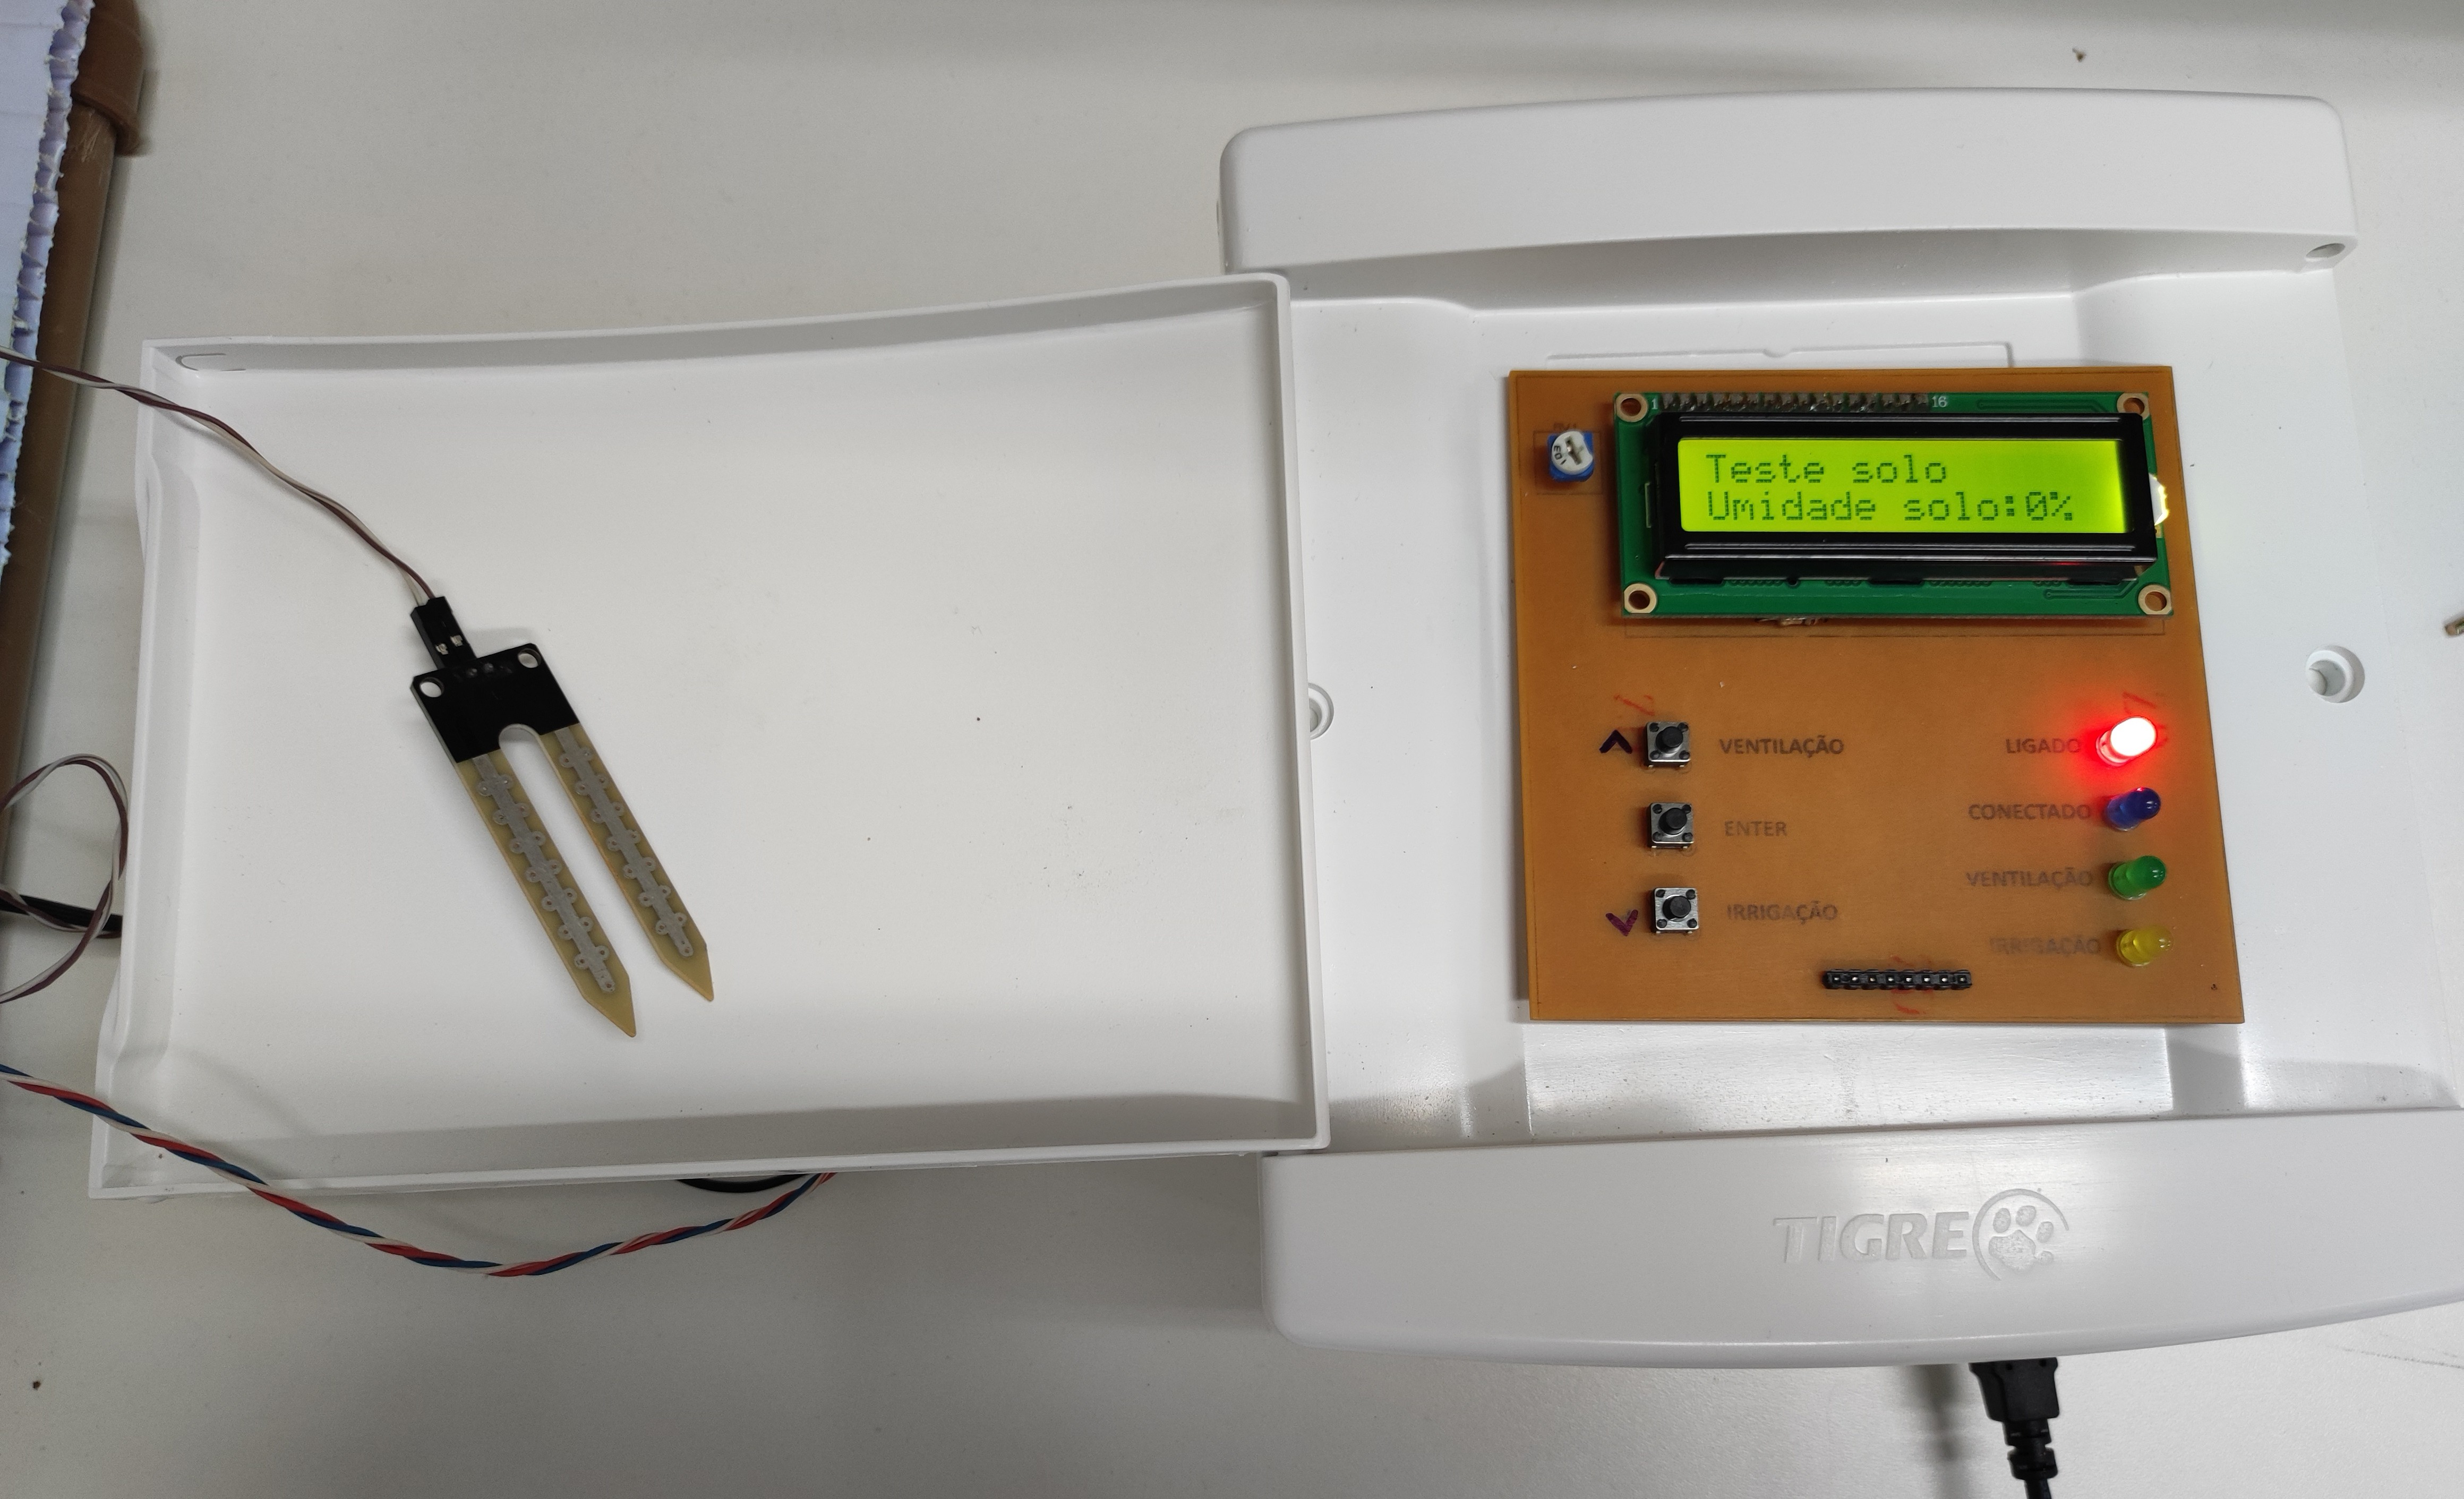
\includegraphics[width=8cm]{figuras/avazio.jpg}\\
% 	\autoria{Autoria Própria}
% 	\label{fig:avazio}
% \end{figure}

% O sensor foi testado em três tipos de solo, sendo eles arenoso, orgânico e argiloso, apresentados na Figura \ref{fig:solos}, que variam a forma com que absorvem a água. Inicialmente os três solos estavam totalmente secos durante a realização das medidas, desse modo, o sensor captou umidade do solo próximo a 0 para os três testes.

% \begin{figure}[!h]
% 	\centering
% 	\caption{Tipos de solo testados}
% 	%\vskip 5mm
% 	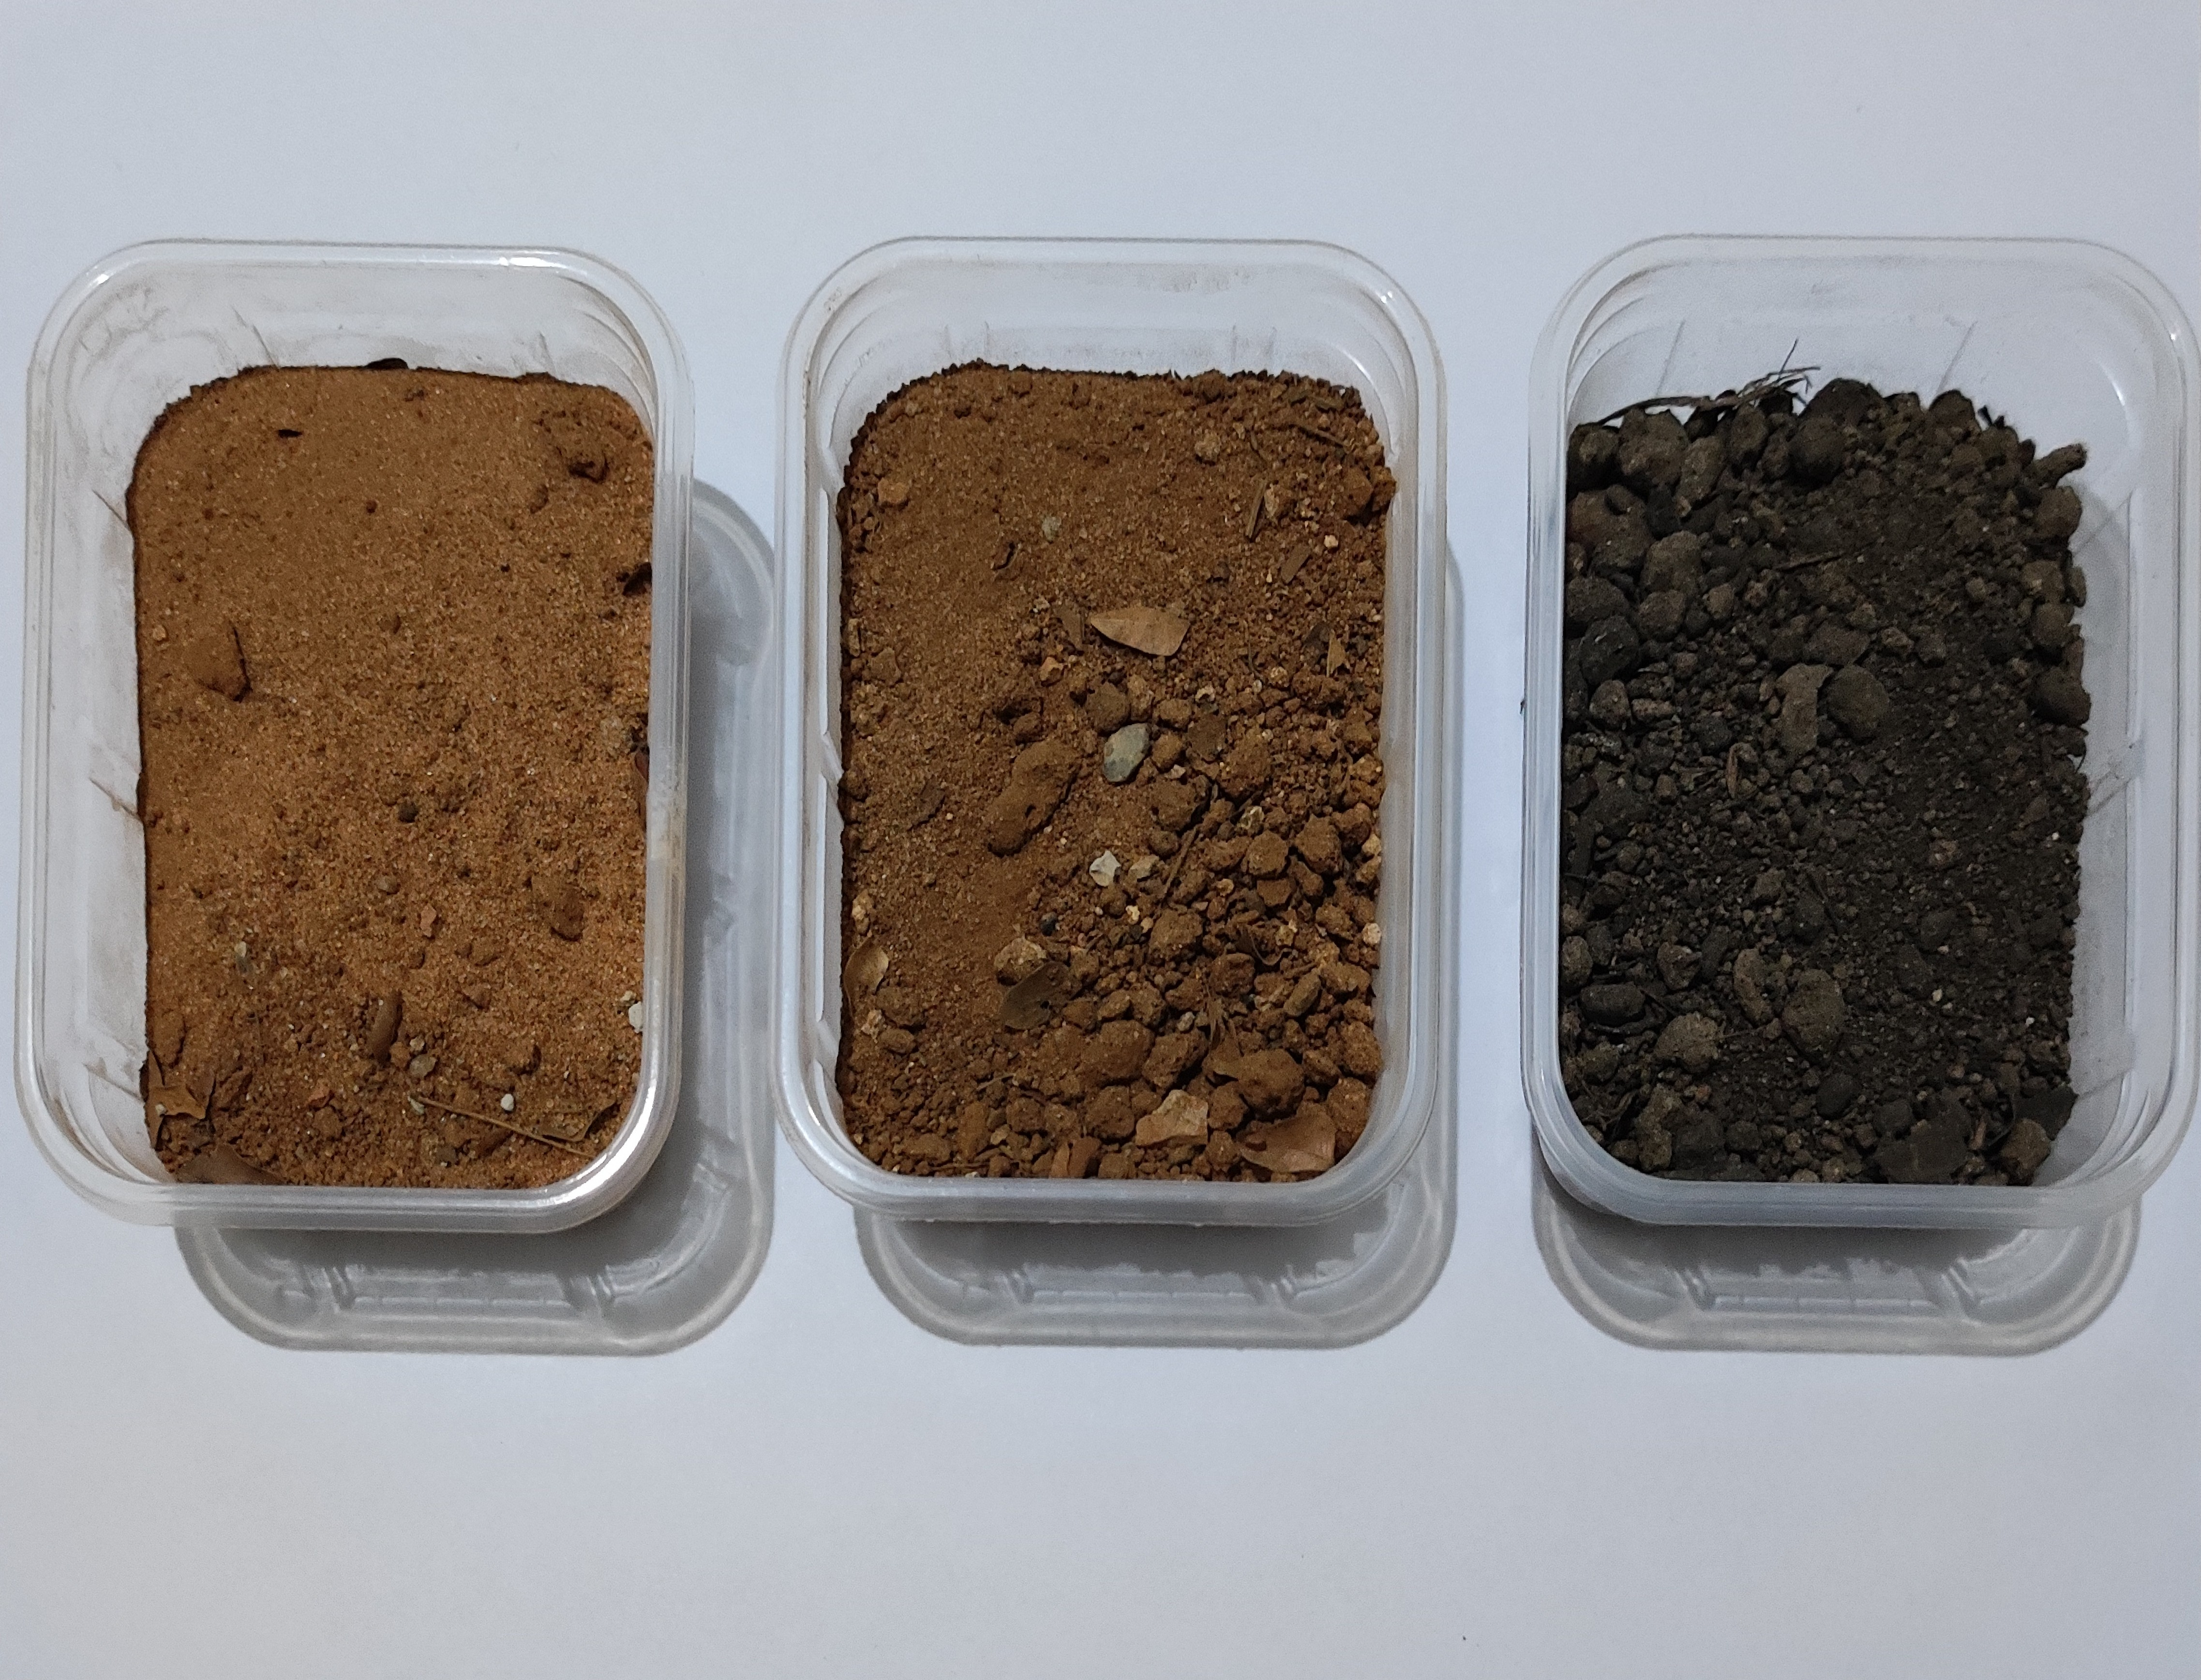
\includegraphics[width=8cm]{figuras/solos.jpg}\\
% 	\autoria{Autoria Própria}
% 	\label{fig:solos}
% \end{figure}

% Em seguida, foi adicionado cerca de 20ml de água nos três recipientes, e foram realizadas novas medidas. Nesse teste, a umidade do solo obtida variou conforme o tipo de solo, sendo que o solo arenoso apresentou maior valor de umidade, por conta da baixa absorção que esse tipo de solo apresenta. 

% Foi adicionado água gradativamente, até o limite da capacidade do recipiente, as medidas foram coletadas, os resultados das medidas foram organizados na Tabela \ref{tab:umidadesolo}. Em seguida o sensor foi mergulhado em água, onde o valor da umidade do solo se tornou 100\%, como esperado.

% \begin{table}[!h]
% \centering
% \caption{Medidas de umidade do solo em três tipos de solo}
% \label{tab:umidadesolo}
% \begin{tabular}{c|c|c|c}
% \hline
% \begin{tabular}[c]{@{}c@{}}Quantidade\\  de água\end{tabular} & \begin{tabular}[c]{@{}c@{}}Solo \\ arenoso\end{tabular} & \begin{tabular}[c]{@{}c@{}}Solo \\ orgânico\end{tabular} & Solo argiloso \\ \hline
% 0 & 0\% & 0\% & 0\% \\ \hline
% 20ml & 18\% & 14\% & 15\% \\ \hline
% 40ml & 39\% & 31\% & 34\% \\ \hline
% 60ml & 62\% & 55\% & 58\% \\ \hline
% 80ml & 85\% & 71\% & 76\% \\ \hline
% \end{tabular}
% \\
% \autoria{Autoria própria}
% \end{table}

% Analisando os dados apresentados, é possível afirmar que o sensor é adequado para a aplicação do presente trabalho, sendo capaz de medir a variação da umidade do solo para diferentes quantidades de água e para variados tipos de solo. 

% \section{Módulo atuador}

% O módulo relé utilizado como atuador neste trabalho permite grande versatilidade no acionamento de cargas, podendo acionar diretamente cargas em corrente contínua e corrente alternada de tensão monofásica, além de poder acionar indiretamente cargas trifásicas, fazendo parte do circuito de controle. Desse modo, os testes para o módulo atuador consistiram em acionar um motor de corrente contínua e um motor de indução trifásico, apresentados na Figura \ref{fig:motores}. 

% \begin{figure}[!h]
% 	\centering
% 	\caption{Testes com motor trifásico e motor de corrente contínua}
% 	%\vskip 5mm
% 	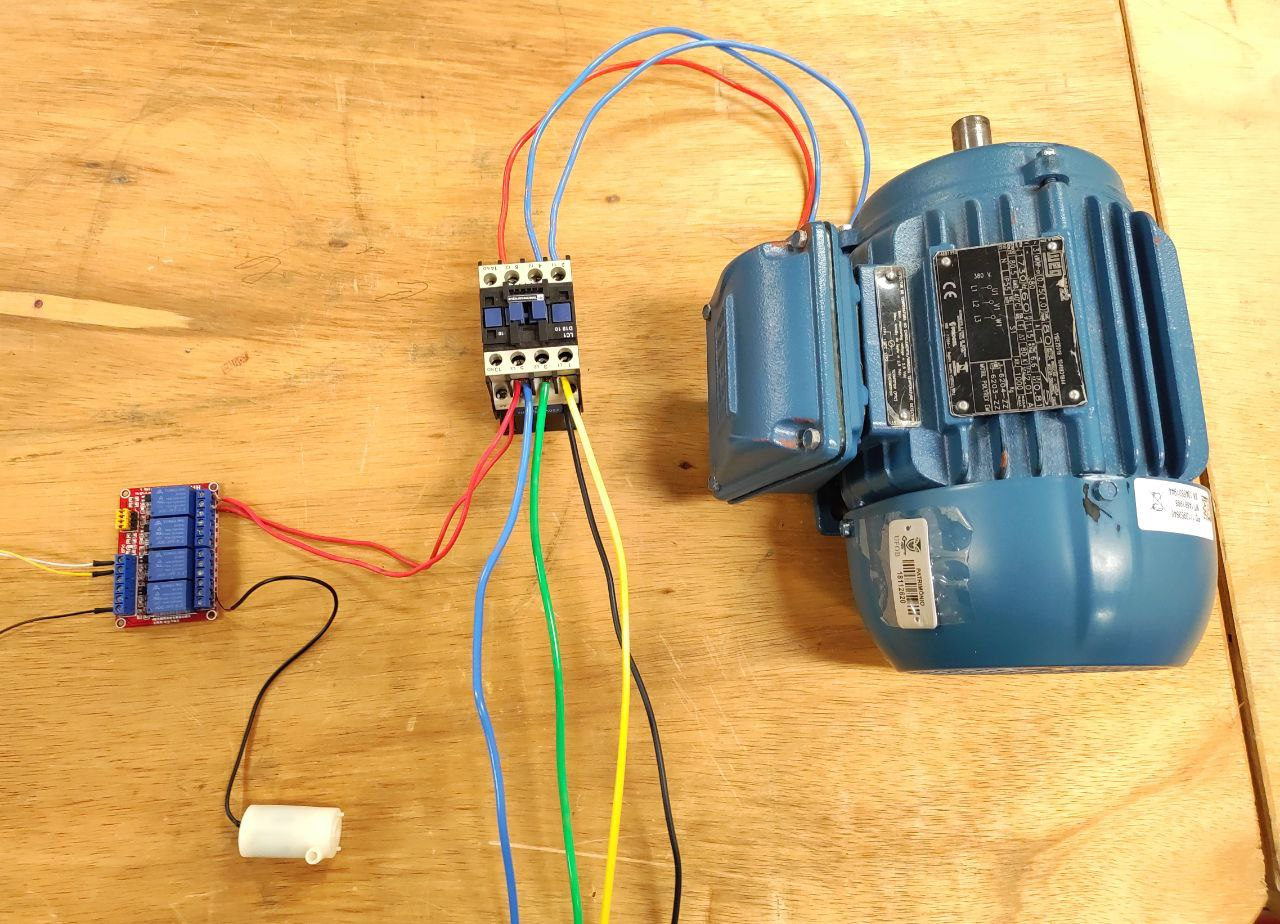
\includegraphics[width=9cm]{figuras/motores.jpg}\\
% 	\autoria{Autoria Própria}
% 	\label{fig:motores}
% \end{figure}

% Para acionar o motor em corrente contínua, foi ligado o terminal positivo de uma fonte de 12V no pino normalmente aberto do relé, o fio positivo do motor foi ligado no pino comum do relé e o fio negativo do motor foi ligado diretamente ao terminal negativo da fonte, como visto no esquema de ligação apresentado na Figura \ref{fig:motorcc}.

% \begin{figure}[!h]
% 	\centering
% 	\caption{Diagrama elétrico de ligação para o motor corrente contínua}
% 	%\vskip 5mm
% 	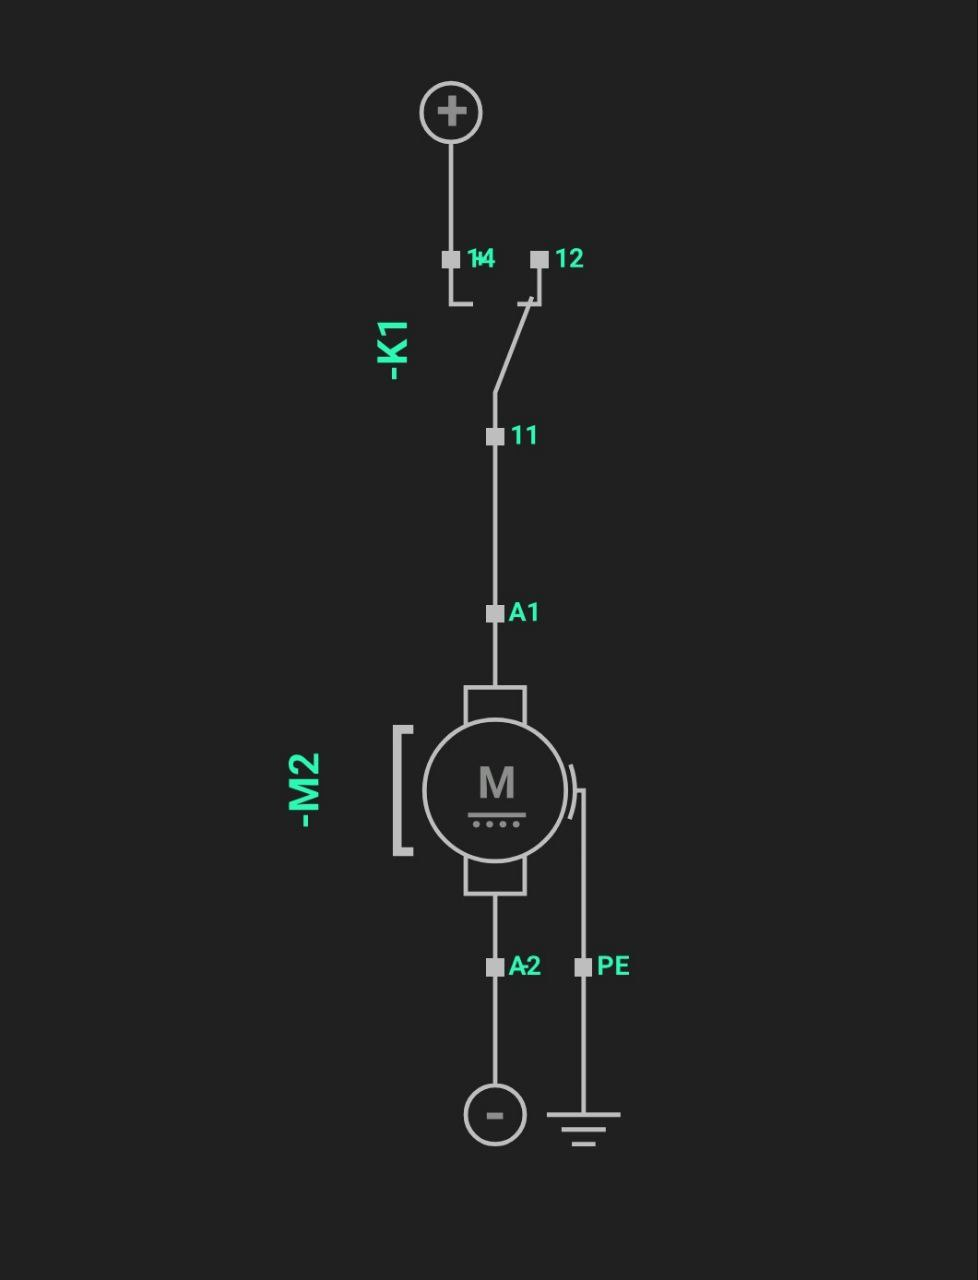
\includegraphics[width=6cm]{figuras/motorcc.jpg}\\
% 	\autoria{Autoria Própria}
% 	\label{fig:motorcc}
% \end{figure}

% O teste de acionamento do motor trifásico foi realizado com o auxílio de um contator, onde o relé foi responsável pelo acionamento da bobina do contator, que por sua vez, acionou o motor trifásico, o esquema de ligação é apresentado na Figura \ref{fig:motorca}.

% \begin{figure}[!h]
% 	\centering
% 	\caption{Diagrama elétrico de ligação para o motor trifásico}
% 	%\vskip 5mm
% 	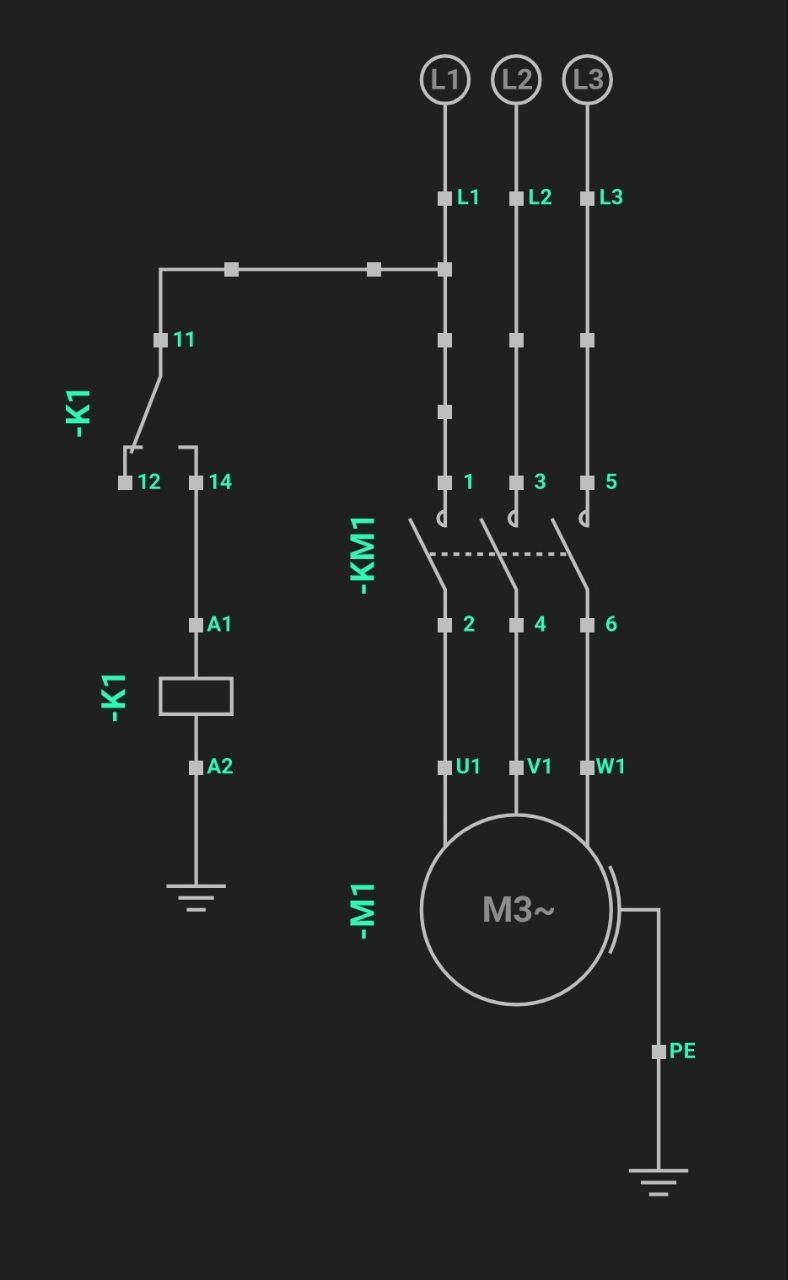
\includegraphics[width=6cm]{figuras/motorca.jpg}\\
% 	\autoria{Autoria Própria}
% 	\label{fig:motorca}
% \end{figure}

% Em ambos os testes foi possível acionar os motores, podendo estes atuar como bombas de irrigação e de ventilação, em pequena e grande escala. Desse modo, o módulo atuador se mostrou eficaz, acionando de maneira rápida e segura as cargas testadas, sedo adequada a sua utilização no projeto.

% \section{Circuito de condicionamento de sinais}

% O circuito de condicionamento de sinais teve seu desempenho testado paralelamente aos testes dos sensores, porém, foram realizados testes específicos para averiguar outras características do seu funcionamento julgadas essenciais para o bom desempenho do sistema como um todo. 

% Ao coletar as informações dos sensores, o circuito tinha como primeira função converter os dados em valores que pudessem ser interpretados e comparados pelo resto do código e pelo usuário. Ao realizar os testes com o sensor de umidade do solo, o circuito de condicionamento de sinais foi capaz de converter o valor analógico enviado pelo sensor em um valor digital em escala decimal, que pôde ser exibido no visor da interface humano/máquina e usado para validação do sensor. 

% Para os teste de temperatura e umidade relativa do ar, o circuito de condicionamento de sinais foi capaz de executar todas as funções cruciais para o funcionamento do sensor DHT-22, sendo capar de interpretar o valor binário de 16 bits enviado pelo sensor e separar os dados de temperatura e umidade do ar, além de converte-los em escala decimal e exibir na IHM. 

% Graças ao bom funcionamento deste circuito, todos os testes realizados entre os módulos foram possíveis, decretando este como o principal componente do sistema, sendo indispensável para o funcionamento do protótipo como um todo. Destarte, este circuito tem seu funcionamento continuado mesmo com a ausência de outros módulos do sistema, como exemplo a conexão via radiofrequência com o módulo central ou a comunicação com a internet, onde o módulo é capaz de funcionar normalmente coletando os dados dos sensores e controlando os atuadores, além de exibir as informações para o usuário por meio da IHM

% Mesmo com a ausência do módulo sensores, o circuito de condicionamento de sinais foi capaz de manter o sistema em funcionamento no modo manual, onde o usuário aciona a ventilação ou irrigação através da IHM. No teste da desconexão com o módulo atuador, o circuito manteve a coleta e envio dos dados dos sensores, mantendo sua funcionalidade como plataforma de monitoramento.

% Todos os teste de validação foram realizados considerando situações extremas, onde alguma parte do sistema teve seu funcionamento comprometido, no entanto, o circuito de condicionamento de sinais foi capaz de manter-se funcionando adequadamente, perdendo apenas a funcionalidade referente à parte desconectada do sistema. Devido a esses resultados, foram adotadas medidas visando manter o circuito de condicionamento de sinais seguro, sendo instalado dentro da caixa de disjuntores e fixado por meio de parafusos, em local inacessível ao usuário do sistema.

% \section{Comunicação por radiofrequência}

% Os testes realizados para validar a comunicação entre o circuito de condicionamento de sinais e o módulo central, que foi realizada através de módulos de radiofrequência consistiu em estabelecer a comunicação e distanciar os módulos até que a comunicação fosse perdida. Foram realizados testes com dois modelos de módulos de radiofrequência diferentes, utilizando antenas diferentes. 

% No primeiro teste, os módulos foram posicionados lado a lado, com o objetivo de estabelece a conexão entre eles, o primeiro modelo testado, apresentado na Figura \ref{fig:hc12}, não estabeleceu conexão, se tornando inutilizável no projeto, os motivos para esse resultado podem estar ligados à uma falsificação dos módulos, já que outros trabalhos foram desenvolvidos com esse mesmo modelo e obtiveram bons resultados de conexão e distancia de transmissão de dados. 

% \begin{figure}[!h]
% 	\centering
% 	\caption{Primeiro modelo de módulo radiofrequência}
% 	%\vskip 5mm
% 	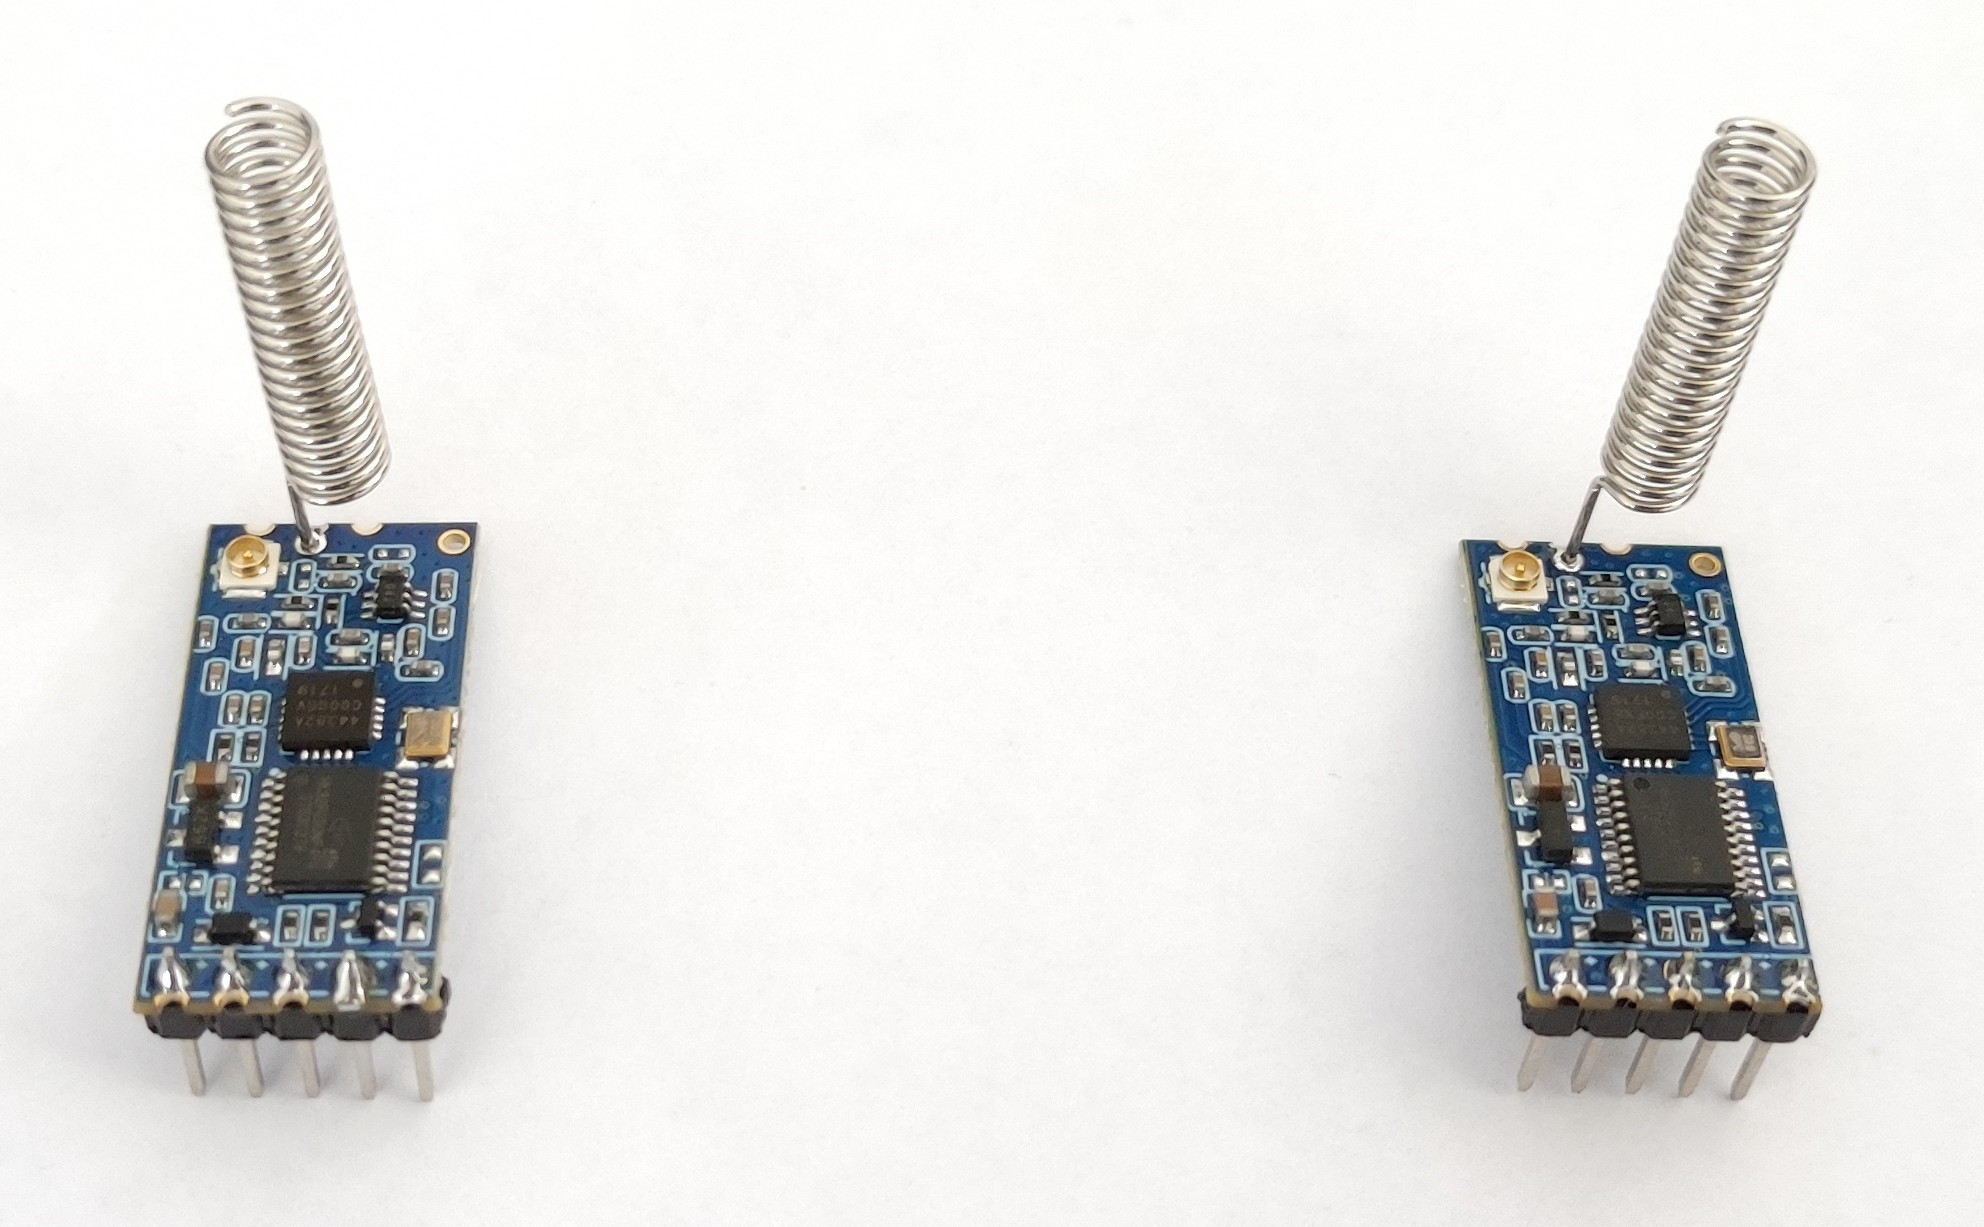
\includegraphics[width=10cm]{figuras/hc12.jpg}\\
% 	\autoria{Autoria Própria}
% 	\label{fig:hc12}
% \end{figure}

% Para o segundo modelo, apresentado na Figura \ref{fig:modrf}, o teste de estabelecimento de conexão obteve êxito, sendo possível transmitir dados entre os módulos. O segundo teste consistiu em distanciar os transmissores em 5 metros e testar a comunicação. Novamente, o segundo módulo conseguiu transmitir os dados entre o circuito de condicionamento de sinais e o módulo central. 

% \begin{figure}[!h]
% 	\centering
% 	\caption{Segundo modelo de módulo radiofrequência}
% 	%\vskip 5mm
% 	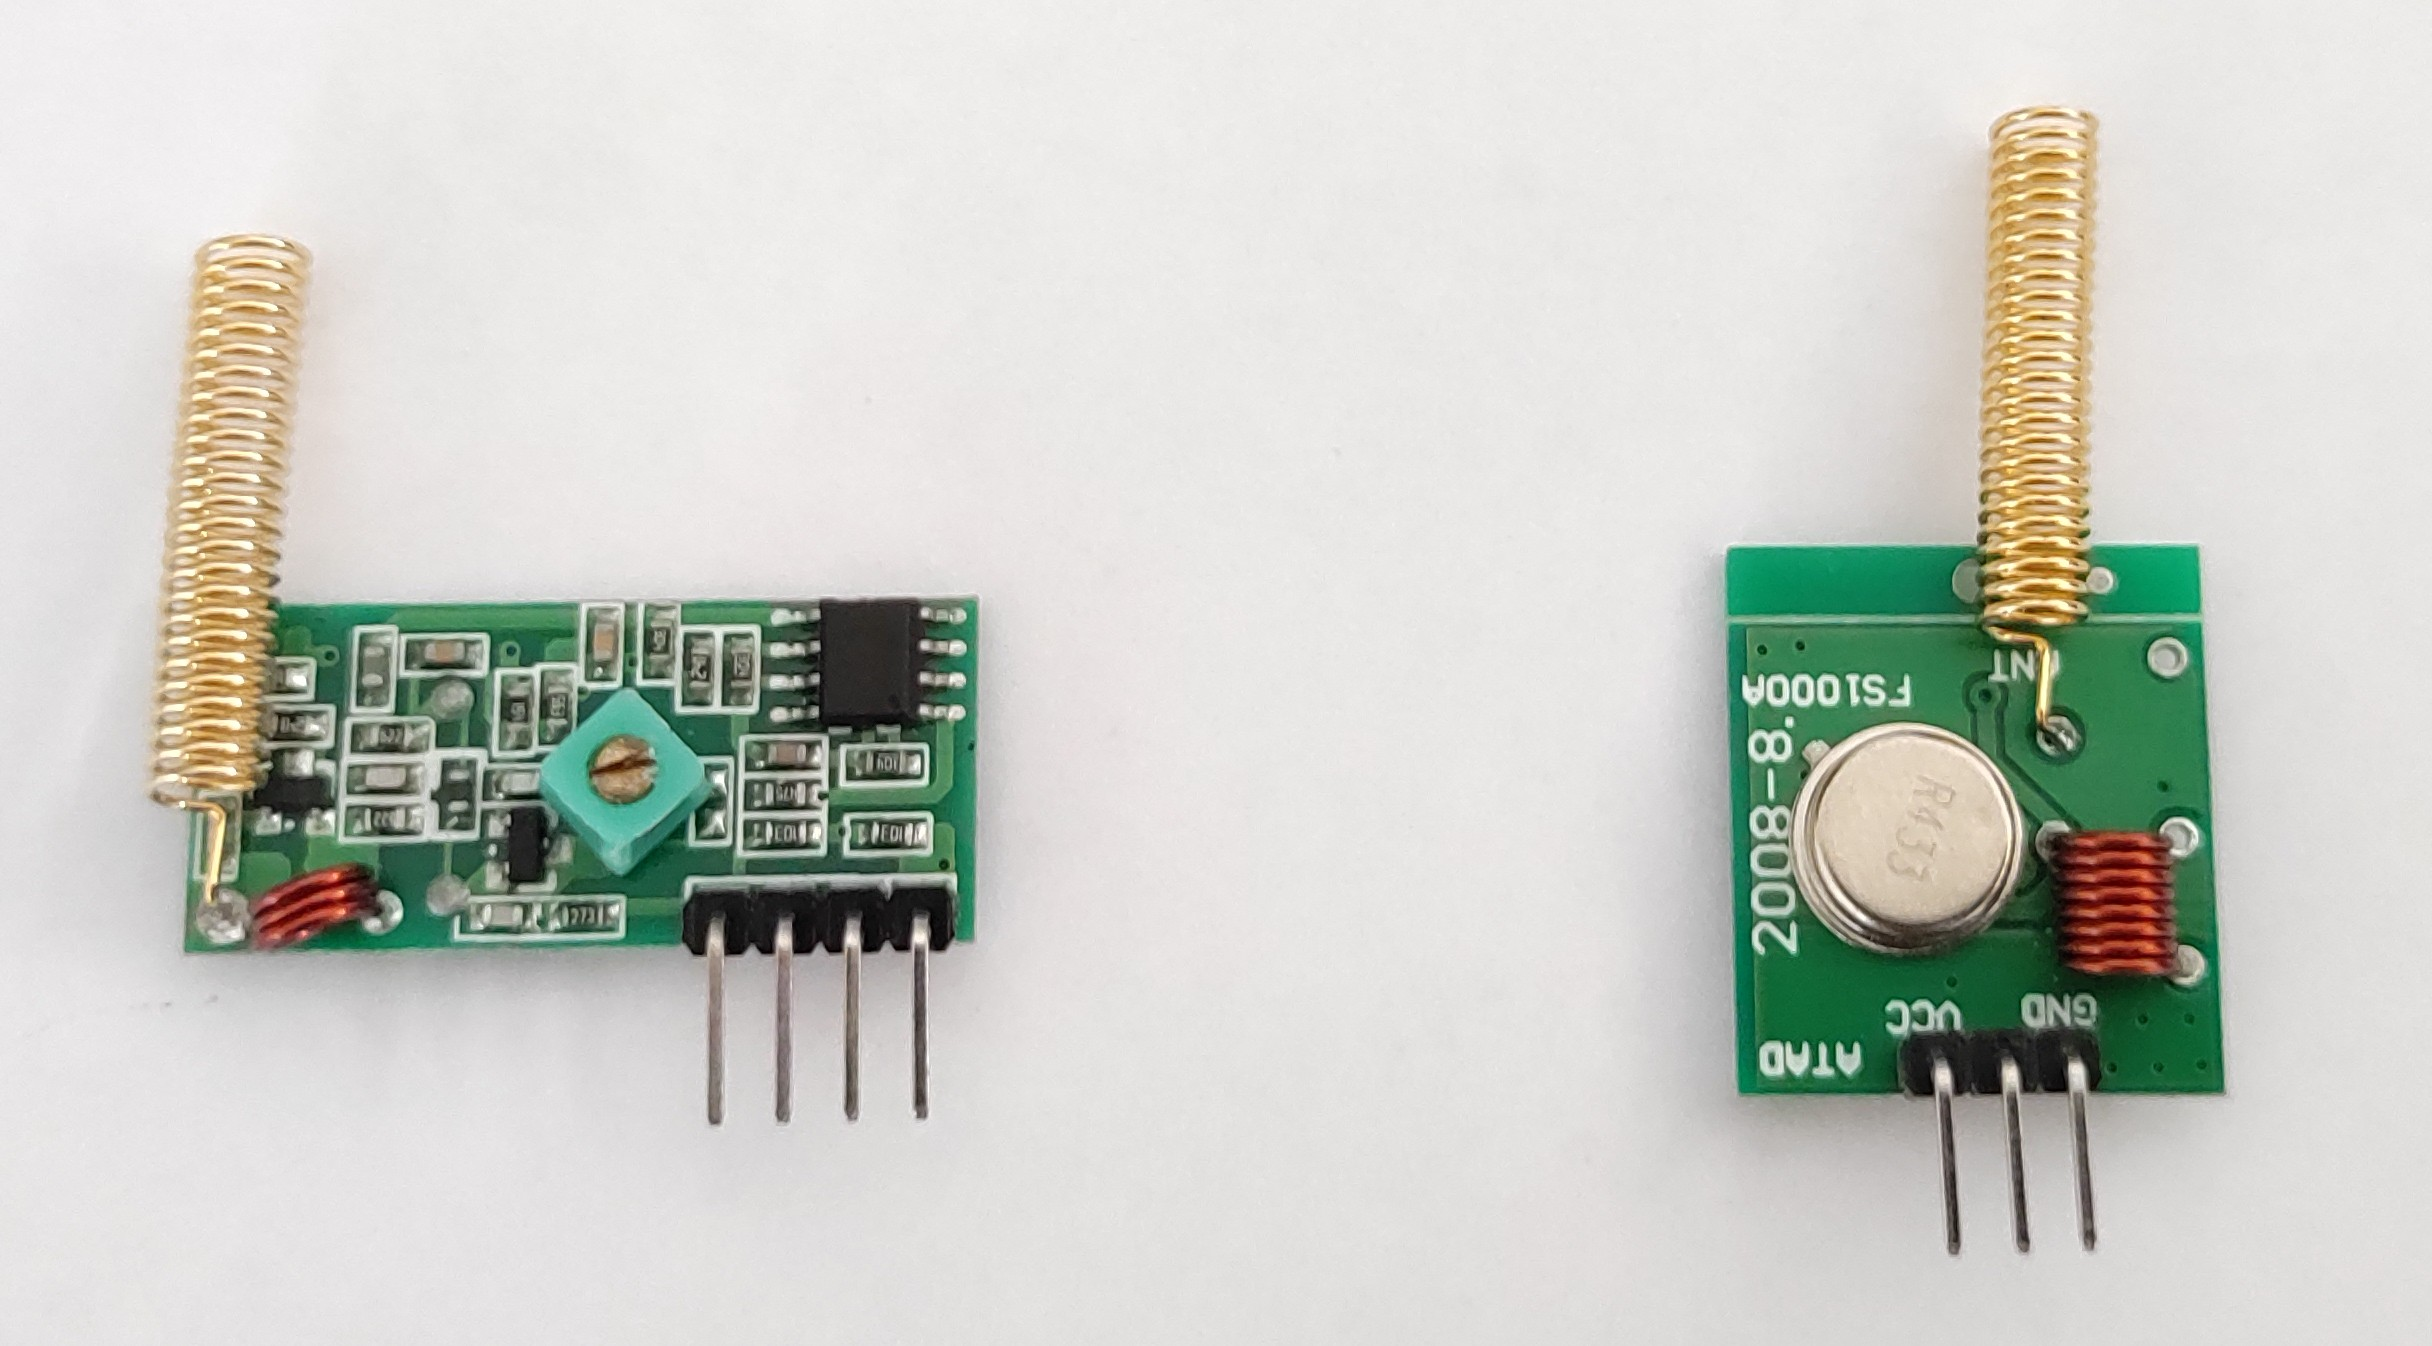
\includegraphics[width=8cm]{figuras/modrf.jpg}\\
% 	\autoria{Autoria Própria}
% 	\label{fig:modrf}
% \end{figure}

% No terceiro teste, os módulos foram separados em 10 metros. Nesta distancia, a comunicação apresentou falhas, onde nem todos os dados enviados pelo circuito de condicionamento de sinais eram recebidos pelo módulo central. O quarto teste consistiu em separar os transmissores em 15 metros, nessa distância a conexão entre os módulos foi perdida. 

% Os resultados obtidos para o segundo modelo de módulo foram como o esperado, considerando as características do transmissor e da antena utilizada. Caso a antena fosse substituída por uma maior, a distância de comunicação poderia ser estendida para cerca de 50 metros. Por conta da baixa distância de transmissão alcançada, optou-se por instalar o módulo central no mesmo recipiente que o circuito de condicionamento de sinais, aproveitando a mesma fonte de alimentação para todo o sistema. Desse modo, todo o sistema pode ser instalado no mesmo ambiente, vale ressaltar que esse resultado não comprometeu o funcionamento do protótipo.

% \section{Módulo central}

% O módulo central tem como principal objetivo intermediar a comunicação entre o sistema e a internet. Por meio deste, é possível acessar as informações do plantio de qualquer lugar do mundo que tenha acesso à internet. Foram realizados testes de conectividade e comunicação através do protocolo MQTT. O protocolo foi implementado no ESP32, por conta do seu módulo wi-fi, sendo conectado à internet e estabelecido contato com o \textit{broker}, em seguida, foi acessado o aplicativo na mesma rede wi-fi em que o módulo central estava conectado e a comunicação foi estabelecida com sucesso. 

% Outros testes foram realizados, sendo eles o acesso ao aplicativo usando uma rede wi-fi diferente da que o módulo central estava conectado e o acesso usando os dados móveis de internet do celular. Em ambos os testes a comunicação foi estabelecida, como apresentado na Figura \ref{fig:telas}.

% \begin{figure}[!h]
% 	\centering
% 	\caption{Comunicação entre o aplicativo}
% 	%\vskip 5mm
% 	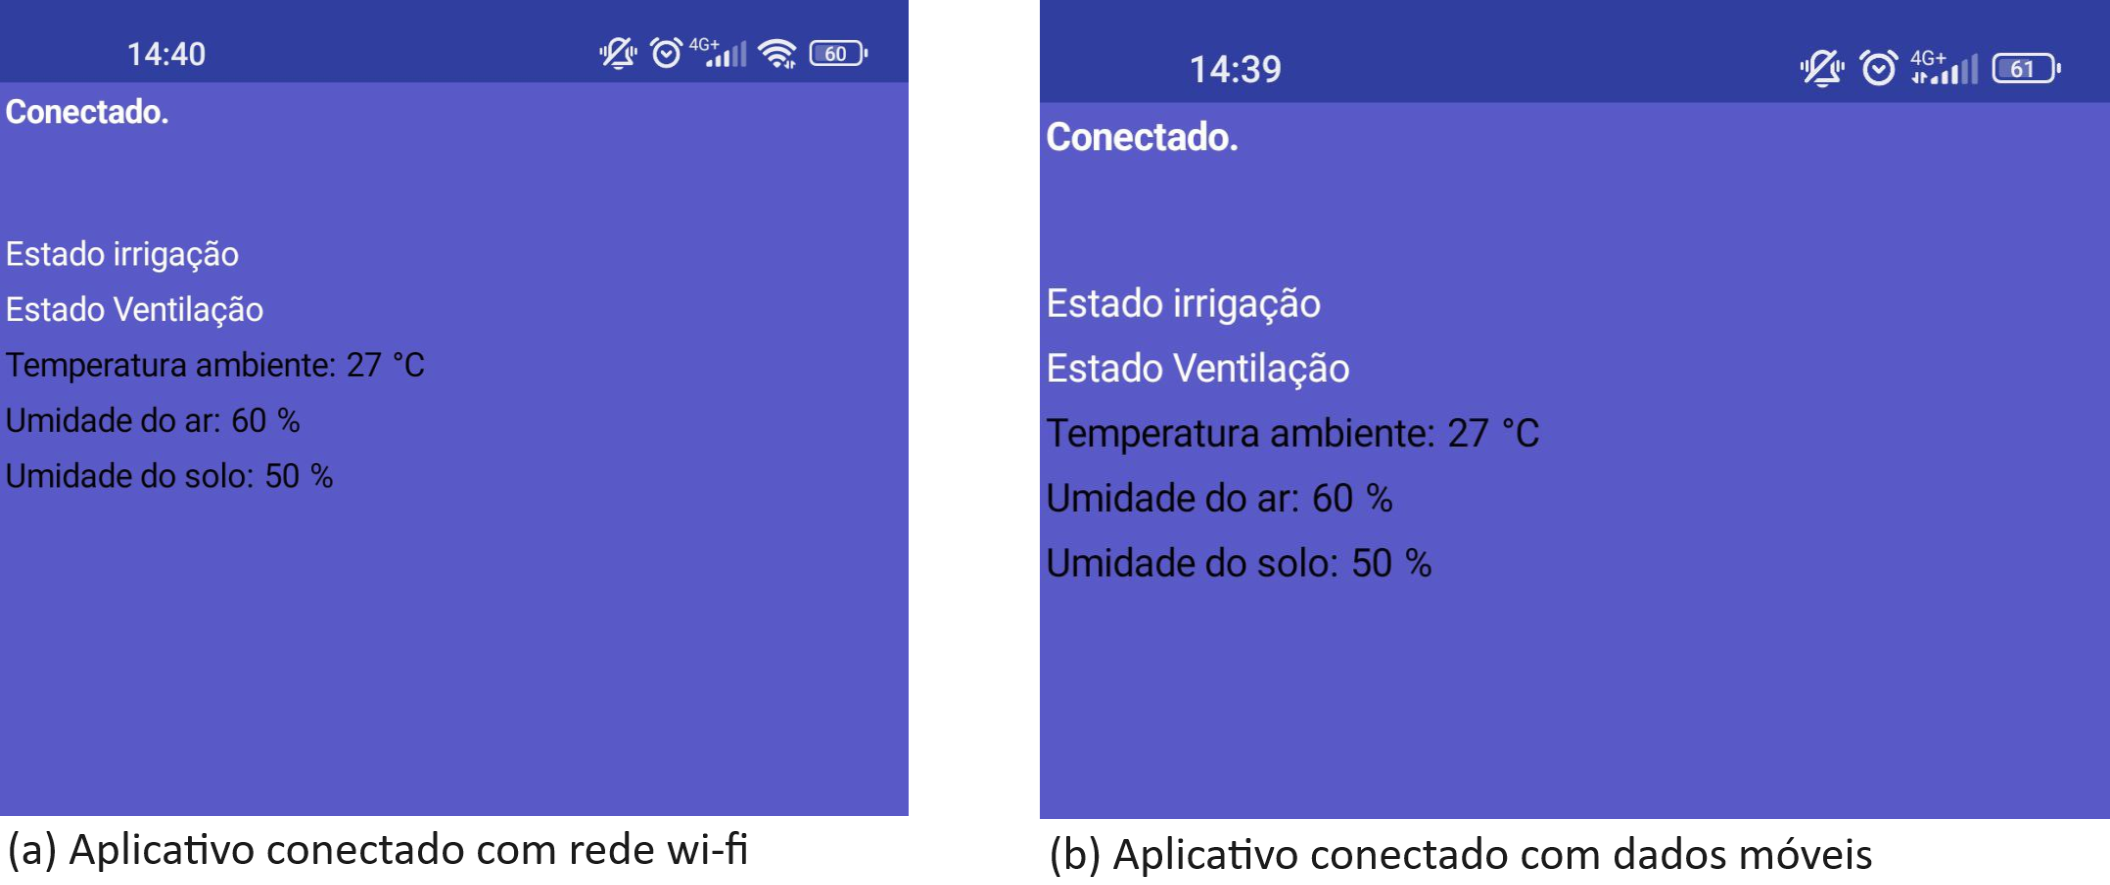
\includegraphics[width=13cm]{figuras/telas.png}\\
% 	\autoria{Autoria Própria}
% 	\label{fig:telas}
% \end{figure}

% Analisando o resultado dos teste, é possível observar que o protocolo MQTT permite uma conexão segura e facilitada, tendo um excelente potencial em aplicações de IoT, permitindo um número ilimitado de dispositivos conectados ao \textit{broker} e possibilitando um tráfego seguro de dados. 

% \section{Teste Prático}

% O protótipo final do trabalho foi montado em uma caixa de disjuntores anti-chamas, com os componentes fixados com parafusos. Todas as conexões entre os módulos foram realizadas dentro da caixa, de maneira que o usuário final não tenha acesso, o processo de montagem é apresentado na Figura \ref{fig:montagem}. 

% \begin{figure}[!h]
% 	\centering
% 	\caption{Montagem do trabalho}
% 	%\vskip 5mm
% 	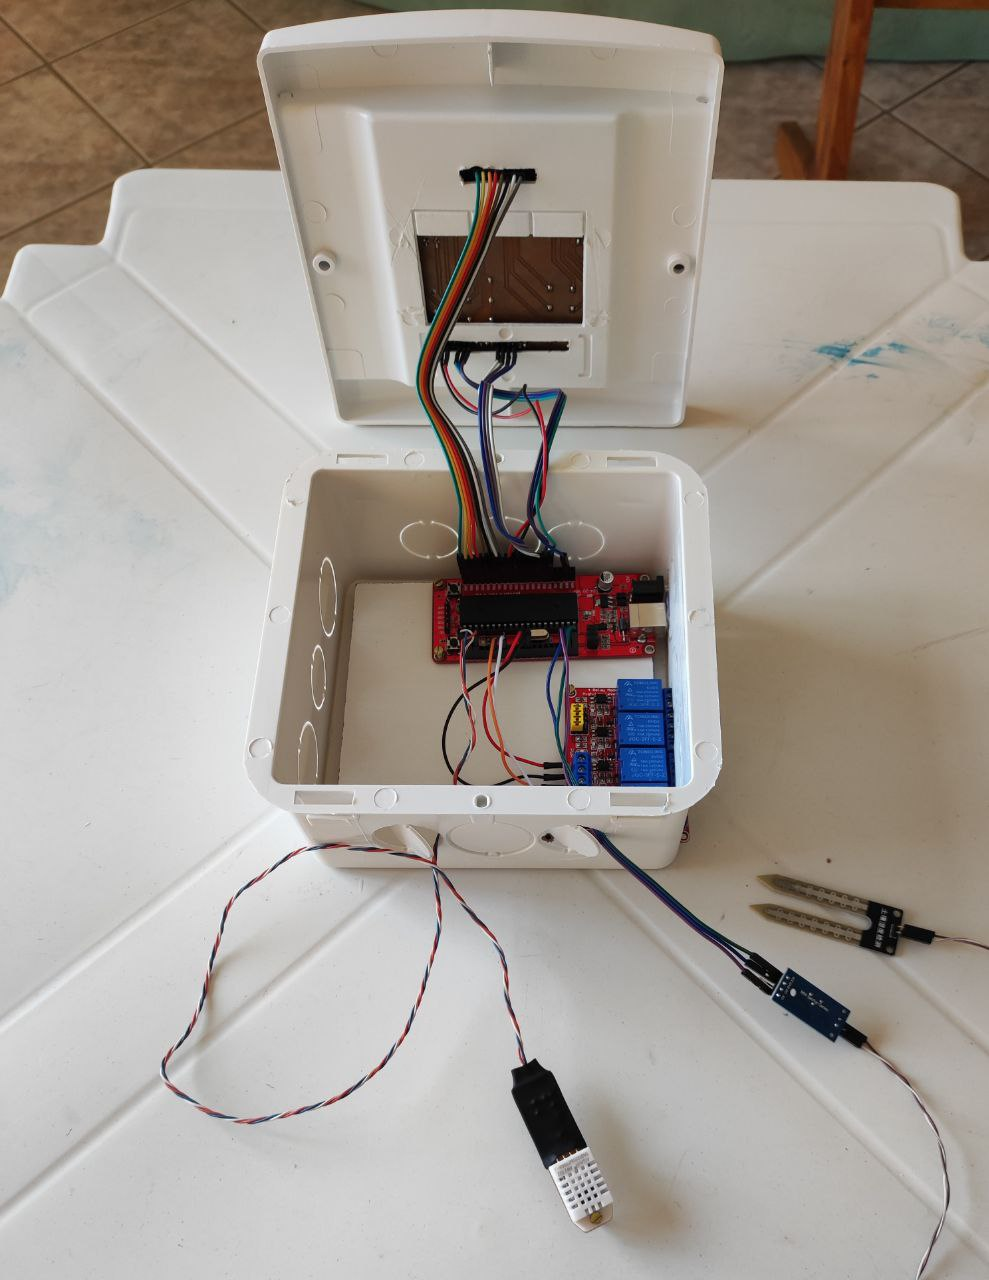
\includegraphics[width=6cm]{figuras/montagem.jpg}\\
% 	\autoria{Autoria Própria}
% 	\label{fig:montagem}
% \end{figure}

% Os módulos foram posicionados de maneira que posse possível a conexão externa dos atuadores e alimentação do sistema. Desse modo, fica disponível ao usuário todas as conexões necessárias para o funcionamento do sistema. Na Figura \ref{fig:releco} são apresentadas as portas de conexão entre o módulo relé e as cargas, tendo seus parafusos de fixação em fácil acesso pelo usuário.

% \begin{figure}[!h]
% 	\centering
% 	\caption{Conexões externas do sistema}
% 	%\vskip 5mm
% 	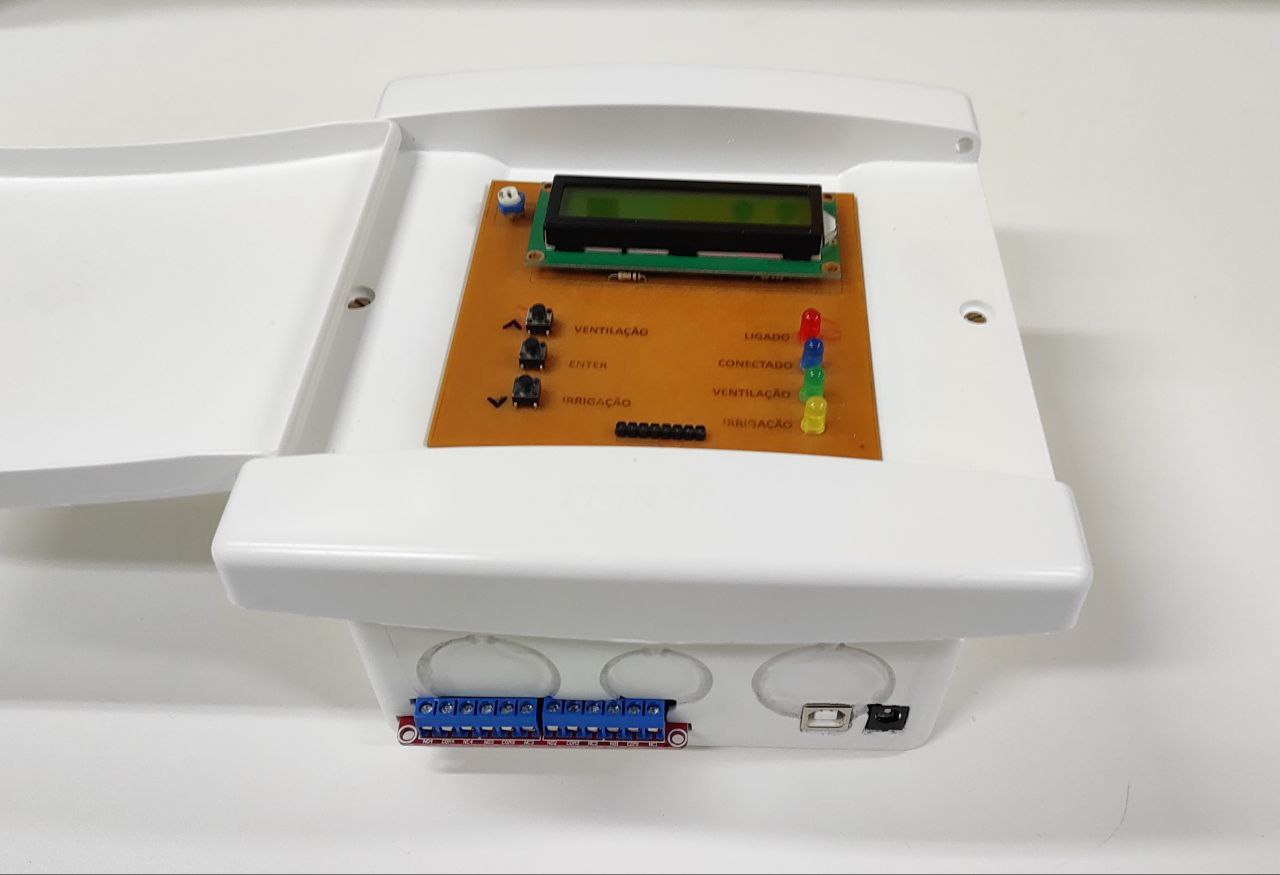
\includegraphics[width=7cm]{figuras/releco.jpg}\\
% 	\autoria{Autoria Própria}
% 	\label{fig:releco}
% \end{figure}

% Os sensores foram conectados internamente ao circuito de condicionamento de sinais e saíram da caixa através de passagens laterais, conforme Figura \ref{fig:saidasensores}.  Desse modo, os sensores podem ser posicionados de acordo com a necessidade do usuário. A maneira com que foi posicionada a saída dos sensores inibe que água escorra para dentro da caixa, protegendo o circuito interno.

% \begin{figure}[!h]
% 	\centering
% 	\caption{Saída dos sensores}
% 	%\vskip 5mm
% 	\includegraphics[width=7cm]{figuras/saidasensores.jpg}\\
% 	\autoria{Autoria Própria}
% 	\label{fig:saidasensores}
% \end{figure}

% A Figura \ref{fig:prontos} apresenta o trabalho com sua montagem finalizada, tendo apenas a interface humano/máquina disponível ao usuário, tornando o sistema mais amigável para pessoas com pouca afinidade à sistema eletrônicos complexos. O sistema pode ser fixado facilmente em paredes, estruturas de madeira, metal ou outro material que possa ser usado para construção de estrutura de estufa. A tampa de proteção inibe que os botões sejam acionados acidentalmente, além de proteger a IHM de fatores externos.

% \begin{figure}[!h]
% 	\centering
% 	\caption{Sistema finalizado}
% 	%\vskip 5mm
% 	\includegraphics[width=12cm]{figuras/prontos.png}\\
% 	\autoria{Autoria Própria}
% 	\label{fig:prontos}
% \end{figure}

% Para a realização dos testes práticos, o sistema foi configurado, através da IHM física, para o plantio de coentro, como apresentado na Figura \ref{fig:coentro}. Desse modo, o sistema assumiu os valores de temperatura e umidade do solo utilizado programados para o coentro.   

% \begin{figure}[!h]
% 	\centering
% 	\caption{Configuração do sistema para o plantio de coentro}
% 	%\vskip 5mm
% 	\includegraphics[width=10cm]{figuras/coentro.jpg}\\
% 	\autoria{Autoria Própria}
% 	\label{fig:coentro}
% \end{figure}

% Após a configuração, os testes realizados utilizaram os valores apresentados na Tabela \ref{tab:parametros}. O sistema tinha como propósito manter a temperatura e umidade do solo entre a faixa estabelecia, devendo acionar e desacionar a irrigação e o sistema de ventilação sempre que necessário e até o valor se encontrar dentro da faixa, respeitando a programação apresentada no capítulo anterior.

% \begin{table}[!h]
% \centering
% \caption{Valores limites para temperatura e umidade do solo}
% \label{tab:parametros}
% \begin{tabular}{c|c|c}
% \hline
% Descrição & Mínimo & Máximo \\ \hline
% Temperatura & 25°C & 35°C \\ \hline
% \begin{tabular}[c]{@{}c@{}}Umidade do\\ solo\end{tabular} & 45\% & 65\% \\ \hline
% \end{tabular}
% \\
% \autoria{Autoria própria}
% \end{table}

% Para a realização dos testes foi desenvolvida estrutura para simular um ambiente de estufa utilizando materiais plásticos. Na Figura~\ref{fig:mont1} é ilustrado o protótipo em fase de desenvolvimento, em que pode-se observar o ventilador ao fundo. 

% \begin{figure}[!h]
% 	\centering
% 	\caption{Estrutura parcial}
% 	%\vskip 5mm
% 	\includegraphics[width=8cm]{figuras/montagem1.png}\\
% 	\autoria{Autoria Própria}
% 	\label{fig:mont1}
% \end{figure}

% Na Figura~\ref{fig:mont2} é observada a estrutura finalizada, contendo em seu interior os sensores de temperatura e umidade do ar, além do sensor de umidade do solo e, ao lado, reservatório contendo água e a bomba submersa.

% \begin{figure}[!h]
% 	\centering
% 	\caption{Estrutura finalizada}
% 	%\vskip 5mm
% 	\includegraphics[width=8cm]{figuras/estufapronta.jpg}\\
% 	\autoria{Autoria Própria}
% 	\label{fig:mont2}
% \end{figure}

% Ao início dos testes, as condições iniciais foram de solo totalmente seco e temperatura ambiente em local externo, exposto ao sol, com temperatura interna à estufa em 38°C, visando simular as condições reais de uma estufa agrícola. Os testes foram realizados ao longo de 4 horas contínuas, onde foram aferidos os valores a cada 5 minutos. 


% Como o solo se apresentava seco, o sistema acionou a irrigação, onde pode-se observar na Figura \ref{fig:graficoumidadesolo} a elevação da umidade do solo até ser atingido o valor estipulado pela programação. No momento em que a umidade do solo atingiu o valor, a irrigação foi desligada, no decorrer do teste, o valor de umidade reduziu gradativamente, por conta da evaporação natural, ao atingir o valor mínimo, a irrigação foi novamente acionada, mantendo o nível sempre na faixa estipulada.

% \begin{figure}[!h]
% 	\centering
% 	\caption{Variação da umidade do solo}
% 	%\vskip 5mm
% 	\includegraphics[width=16cm]{figuras/graficoumidadesolo.png}\\
% 	\autoria{Autoria Própria}
% 	\label{fig:graficoumidadesolo}
% \end{figure}

% De acordo com a variação da umidade do solo, o sistema realizou o controle do módulo atuador, onde o estado da bomba de irrigação é apresentado na Figura \ref{fig:graficoirrig}. Nota-se que o acionamento da irrigação foi realizado apenas quando necessário, evitando o uso desnecessário de água. Foi possível observar a eficácia da programação orientada a evitar o acionamento indevido em torno dos valores limites, evitando a danificação do equipamento.

% \begin{figure}[!h]
% 	\centering
% 	\caption{Variação do estado da irrigação}
% 	%\vskip 5mm
% 	\includegraphics[width=16cm]{figuras/graficoestadoirrig.png}\\
% 	\autoria{Autoria Própria}
% 	\label{fig:graficoirrig}
% \end{figure}

% A variação da temperatura durante o teste ocorreu de maneira lenta e gradativa, devido ao ventilador usado ser de baixa potência, porém, O sistema foi capaz de manter o valor dentro da faixa estipulada em programação para o cultivo de coentro. A Figura \ref{fig:temp} apresenta a variação da temperatura medida pelo sensor, nota-se que inicialmente a temperatura estava acima da faixa ideal, sendo imediatamente acionada a ventilação. O sistema foi programado para reduzir a temperatura até o limite mínimo definido, visando aumentar o tempo em que o sistema permanece no valor ideal, sem que haja a necessidade da ventilação permanecer acionada. 

% \begin{figure}[!h]
% 	\centering
% 	\caption{Variação da temperatura}
% 	%\vskip 5mm
% 	\includegraphics[width=16cm]{figuras/graficotemp.jpg}\\
% 	\autoria{Autoria Própria}
% 	\label{fig:temp}
% \end{figure}

% Do mesmo modo que o acionamento da irrigação, a ventilação foi acionada apenas quando necessário, até que a temperatura atingisse o nível estipulado. A Figura \ref{fig:estv} apresenta o estado do ventilador ao longo do teste. ao analisar os dados apresentados, é possível prever o comportamento do sistema de ventilação de acordo com a média de temperatura ambiente do local de instalação do sistema e também a faixa de temperatura ideal do plantio escolhido, permitindo escolher o melhor sistema de ventilação ou refrigeração a ser aplicado à estufa.

% \begin{figure}[!h]
% 	\centering
% 	\caption{Variação do estado da ventilação}
% 	%\vskip 5mm
% 	\includegraphics[width=16cm]{figuras/graficoestadovent.png}\\
% 	\autoria{Autoria Própria}
% 	\label{fig:estv}
% \end{figure}


% Desta forma, os testes comprovam a eficácia do sistema desenvolvido com relação ao controle e automação da irrigação. Vale destacar que a única intervenção necessária do usuário é na etapa de escolha do plantio, reduzindo o tempo e trabalho gastos durante o processo de irrigação. O sistema foi capaz de manter os níveis de temperatura e umidade do solo dentro da faixa ideal escolhida, permitindo a maximização da produção e reduzindo o uso de insumos agrícolas.
	\newpage \thispagestyle{empty}
	
	%\chapter{Trabalhos Futuros}{}
%\label{cap:06}
\chapter{CONCLUSÃO}{}
\label{cap:06}
O sistema desenvolvido nesse trabalho apresentou um método de classificação de doenças em plantações de bananeiras utilizando \ac{RNC}, com foco na identificação da Sigatoka, uma das doenças mais prejudiciais ao cultivo da banana.

Um conjunto robusto de imagens foi fundamental para preparar inicialmente o modelo. A aplicação de técnicas de ampliação de dados e pequenos ajustes de parâmetros foi realizada para melhorar o desempenho da rede, garantindo uma base sólida antes de iniciar o treinamento para a classificação de folhas infectadas.

Após o treinamento da rede, iniciou-se a etapa de avaliação dos resultados, utilizando as métricas de avaliação de \ac{Ac} e \ac{MC} na fase de teste. Os resultados de classificação foram condizentes, com o melhor desempenho atingindo aproximadamente 90\% de \ac{Ac} e um erro próximo de zero. O aumento no número de épocas poderia melhorar ainda mais a precisão em \ac{RNC}s, porém, deve-se considerar o custo-benefício desse incremento, levando em conta o custo de processamento, uma vez que a AlexNet, sendo uma \ac{RNC}, demanda muito tempo de execução.



Para trabalhos futuros, pretende-se aumentar o número de classes de doenças em plantações de bananeiras, para que o sistema possa identificar uma maior variedade aumentando assim a aplicabilidade e robustez do modelo. Além disso, explorar uma implementação de técnicas de pré e pós-processamento, com intuito de otimizar tanto as imagens de entrada quanto o refinamento dos resultados gerados pela rede. Essas melhorias visam elevar a precisão das \ac{RNC}s e torná-los mais eficiente. Outrossim, fazer os testes com imagens tiradas nas condições do ambiente do Projeto Formoso, oferecendo um suporte para o agricultor no monitoramento dessas doenças.


	\newpage \thispagestyle{empty}
	
	%\backmatter % marca o início da parte pós-textual
 	%\bibliographystyle{abntex2-alf}
 	\bibliography{___postextual/CorujaTexReferencias}
 	\addcontentsline{toc}{chapter}{REFERÊNCIAS} % lista as referências no sumário
 	\newpage \thispagestyle{empty}
 	
 	\appendix
 	
 	%\addcontentsline{toc}{chapter}{Apêndice}
%\chapter{Apêndice A}
%\label{apendice:01}

%\section{Apêndice A}

	


%\section{Seção do apêndice}
	
 	\newpage \thispagestyle{empty}
 	
 	\anexo
 	
 	%\addcontentsline{toc}{chapter}{Anexo}
%\chapter{Título do anexo}{}
%\label{anexo:01}
%\section{Seção do anexo}

 	\newpage \thispagestyle{empty}
 	
 	\colophon
\end{document}	



%	\input{filename} imports the commands from filename.tex into the target file; it's equivalent to typing all the commands from filename.tex right into the current file where the \input line is.
%	
%	\include{filename} essentially does a \clearpage before and after \input{filename}, together with some magic to switch to another .aux file, and omits the inclusion at all if you have an \includeonly without the filename in the argument. This is primarily useful when you have a big project on a slow computer; changing one of the include targets won't force you to regenerate the outputs of all the rest.
%	
%\input{Lista_AAS.tex} % inserir lista de abreviaturas, acrônimos e siglas